\chapter{\textsc{Redes de Coautoria}}~\label{redes}
\lhead{\textsc{Redes}}

As características propostas na plotagem da rede é, formato em círculo para fins comparativos, disposição dos vértices com coloração das UF pertencentes a mesma região geográfica, espessura e coloração das arestas indicando o maior volume/peso das coautorias existente entre as UFs, espessuras dos laços, indicando peso das coautorias existentes na mesma UF.


\section{\textbf{Health Sciences}}

\subsubsection{Rede de Coautoria das Universidade Federais do Brasil}


\begin{figure}[H]
	\begin{tabular}{ccc}
		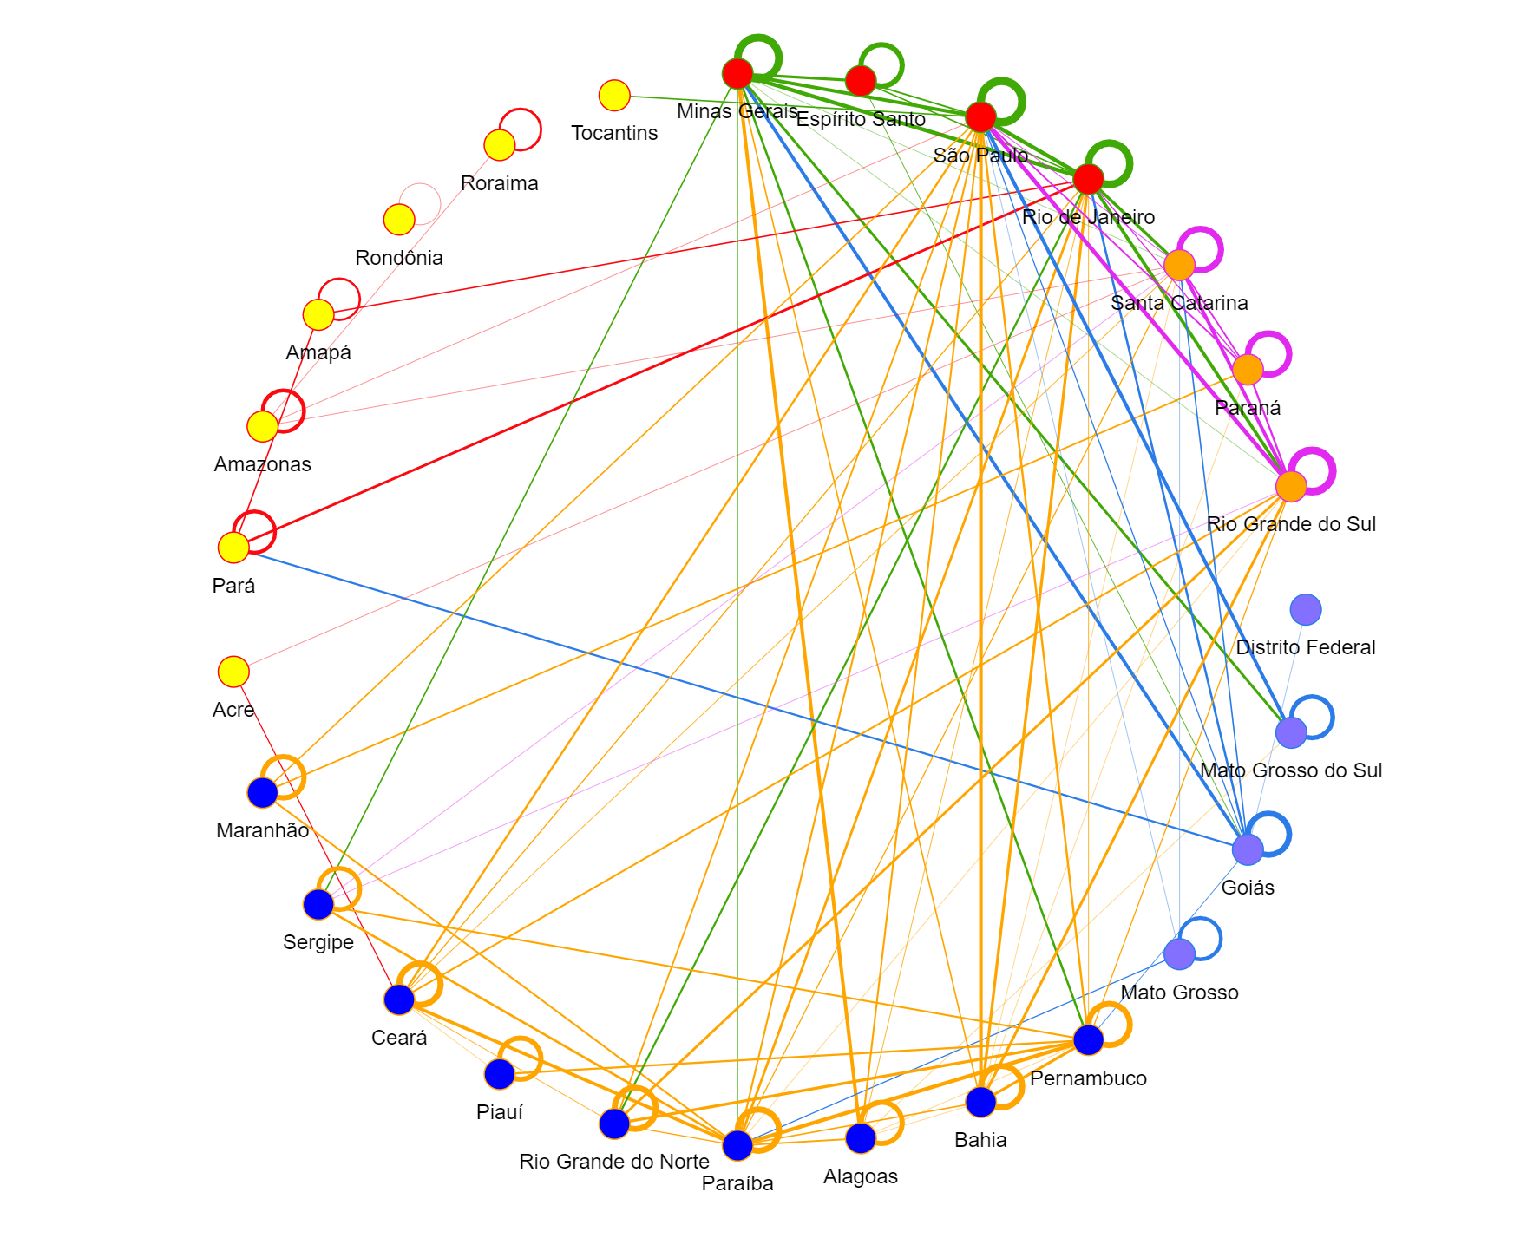
\includegraphics[width=0.35\textwidth]{Imagens/rede-2008.pdf} &   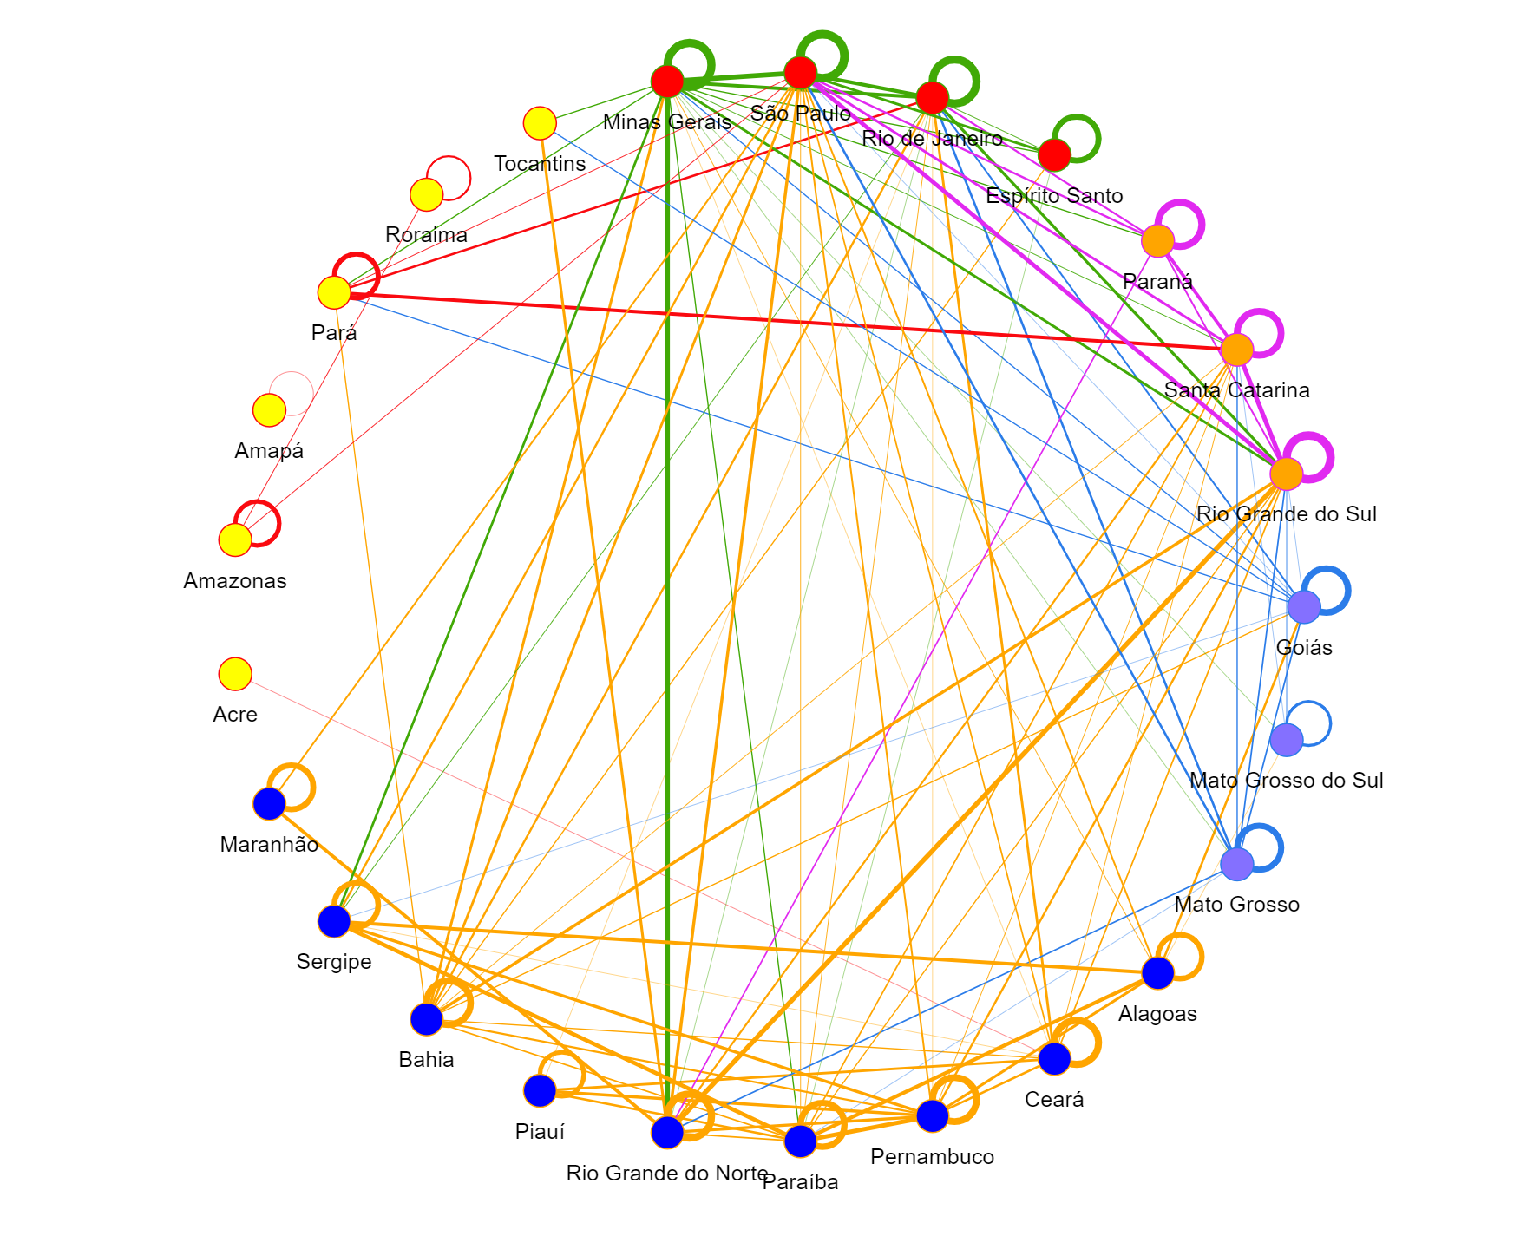
\includegraphics[width=0.35\textwidth]{Imagens/rede-2009.pdf} &
		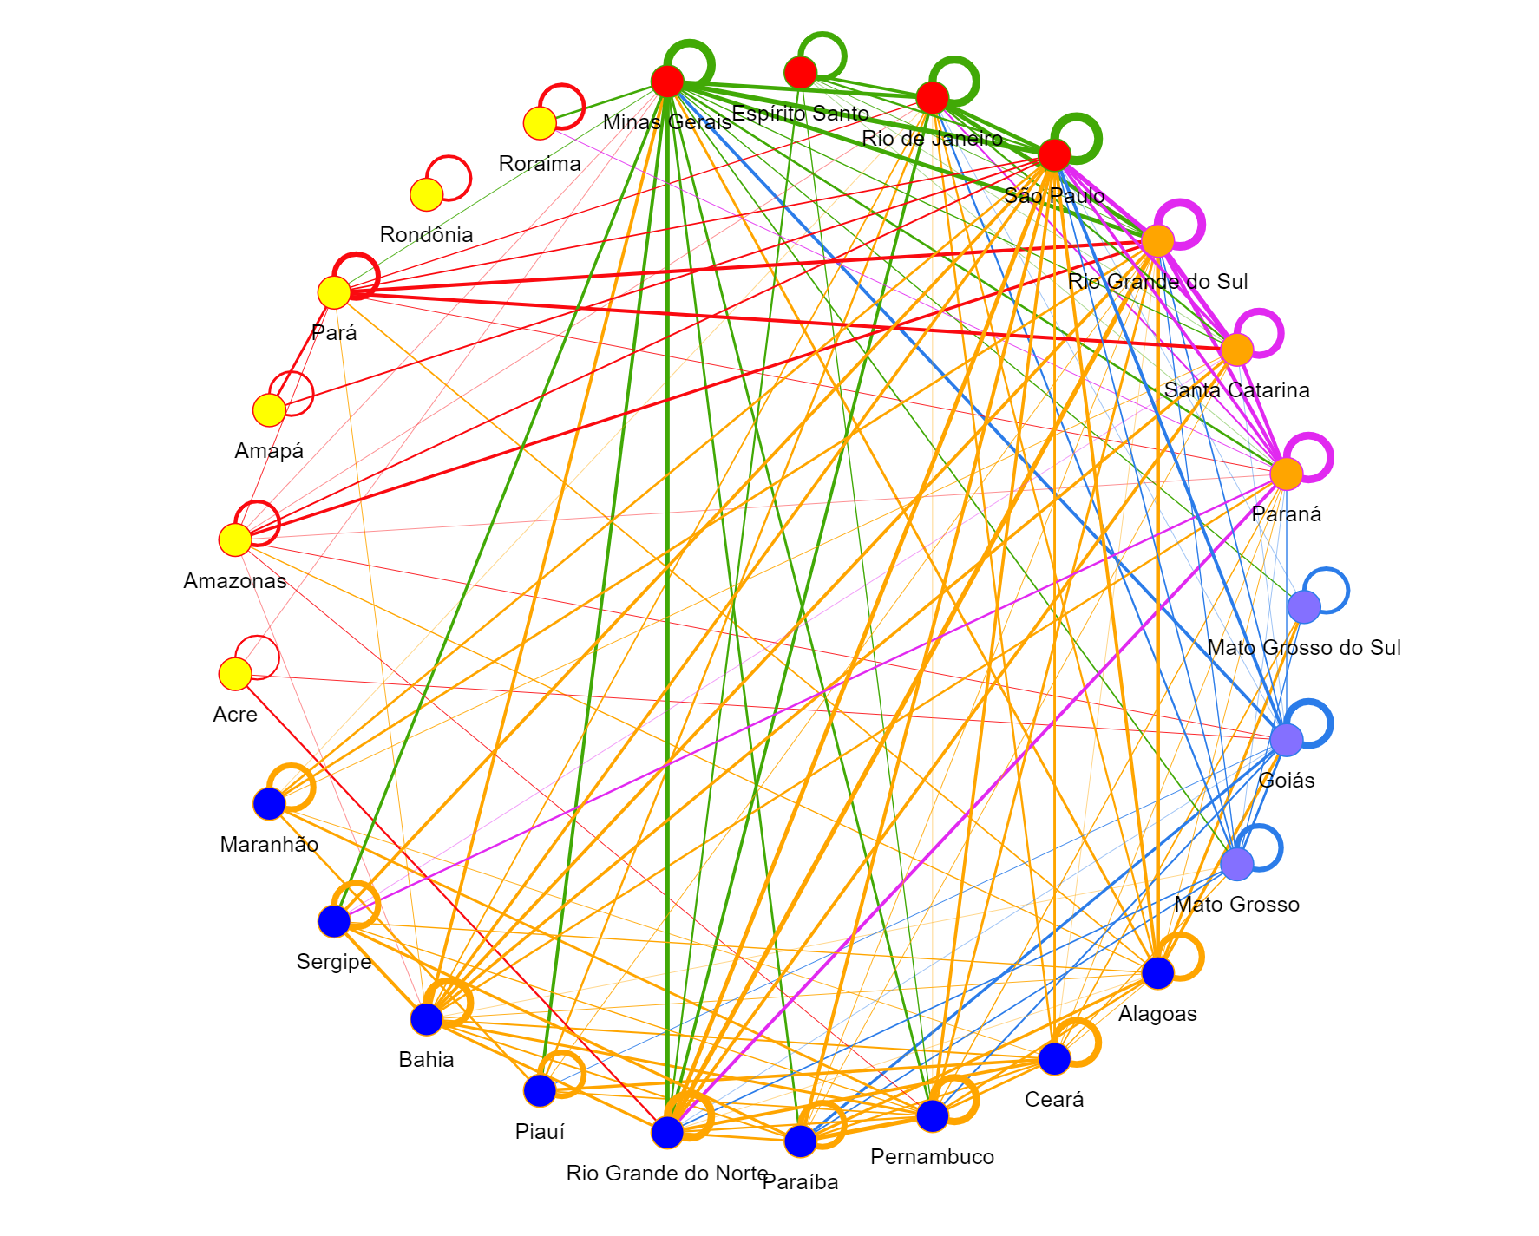
\includegraphics[width=0.35\textwidth]{Imagens/rede-2010.pdf}\\
		2008 & 2009 & 2010\\[6pt] 
		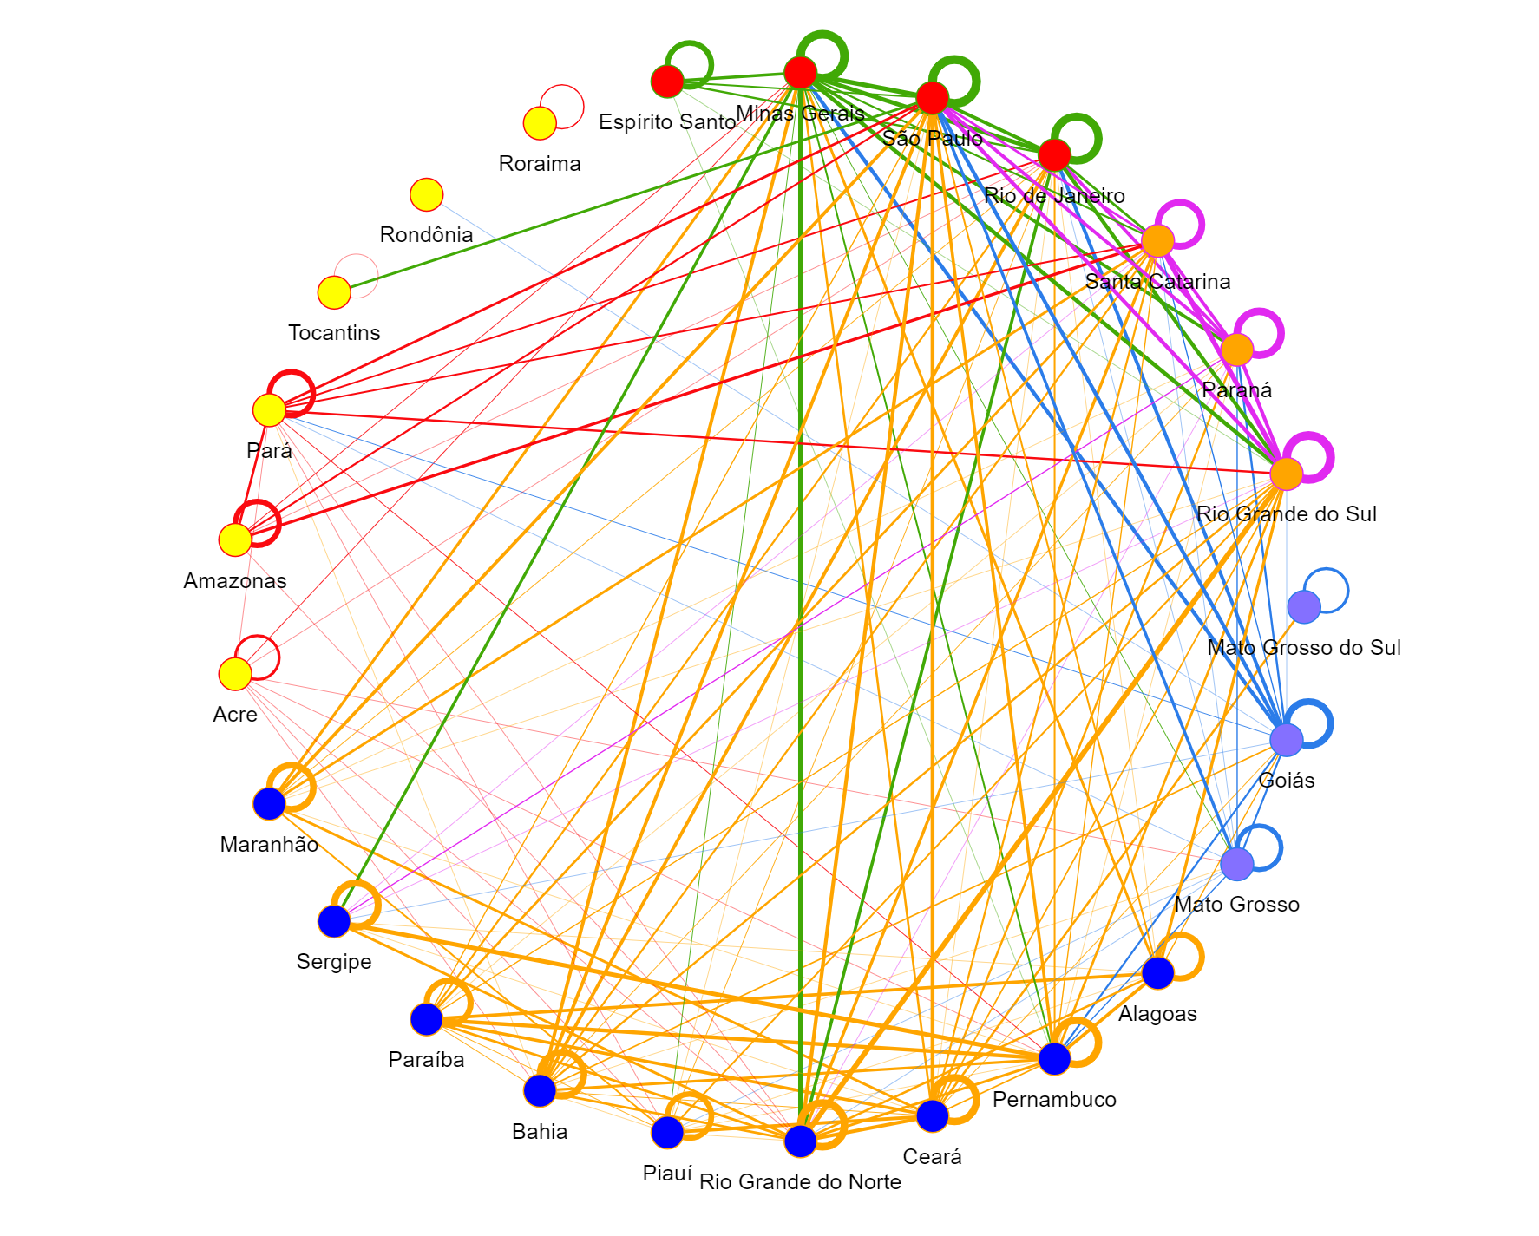
\includegraphics[width=0.35\textwidth]{Imagens/rede-2011.pdf} &
		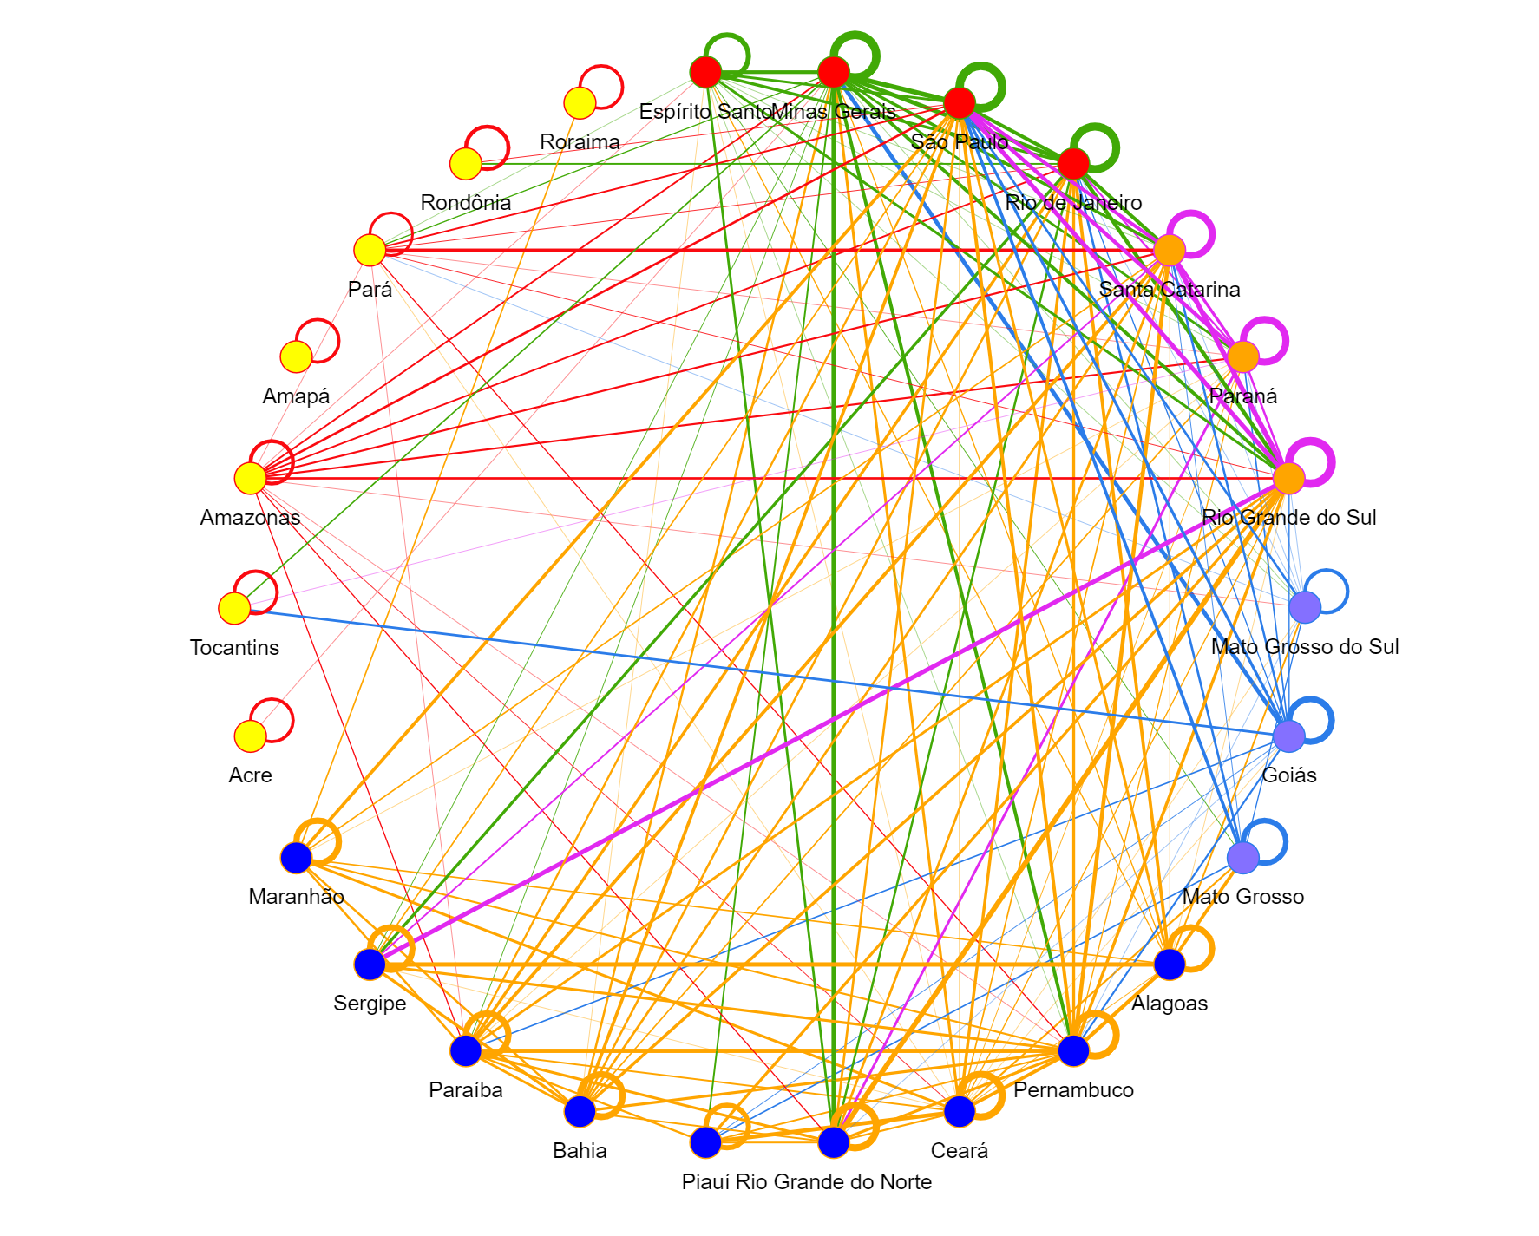
\includegraphics[width=0.35\textwidth]{Imagens/rede-2012.pdf} &   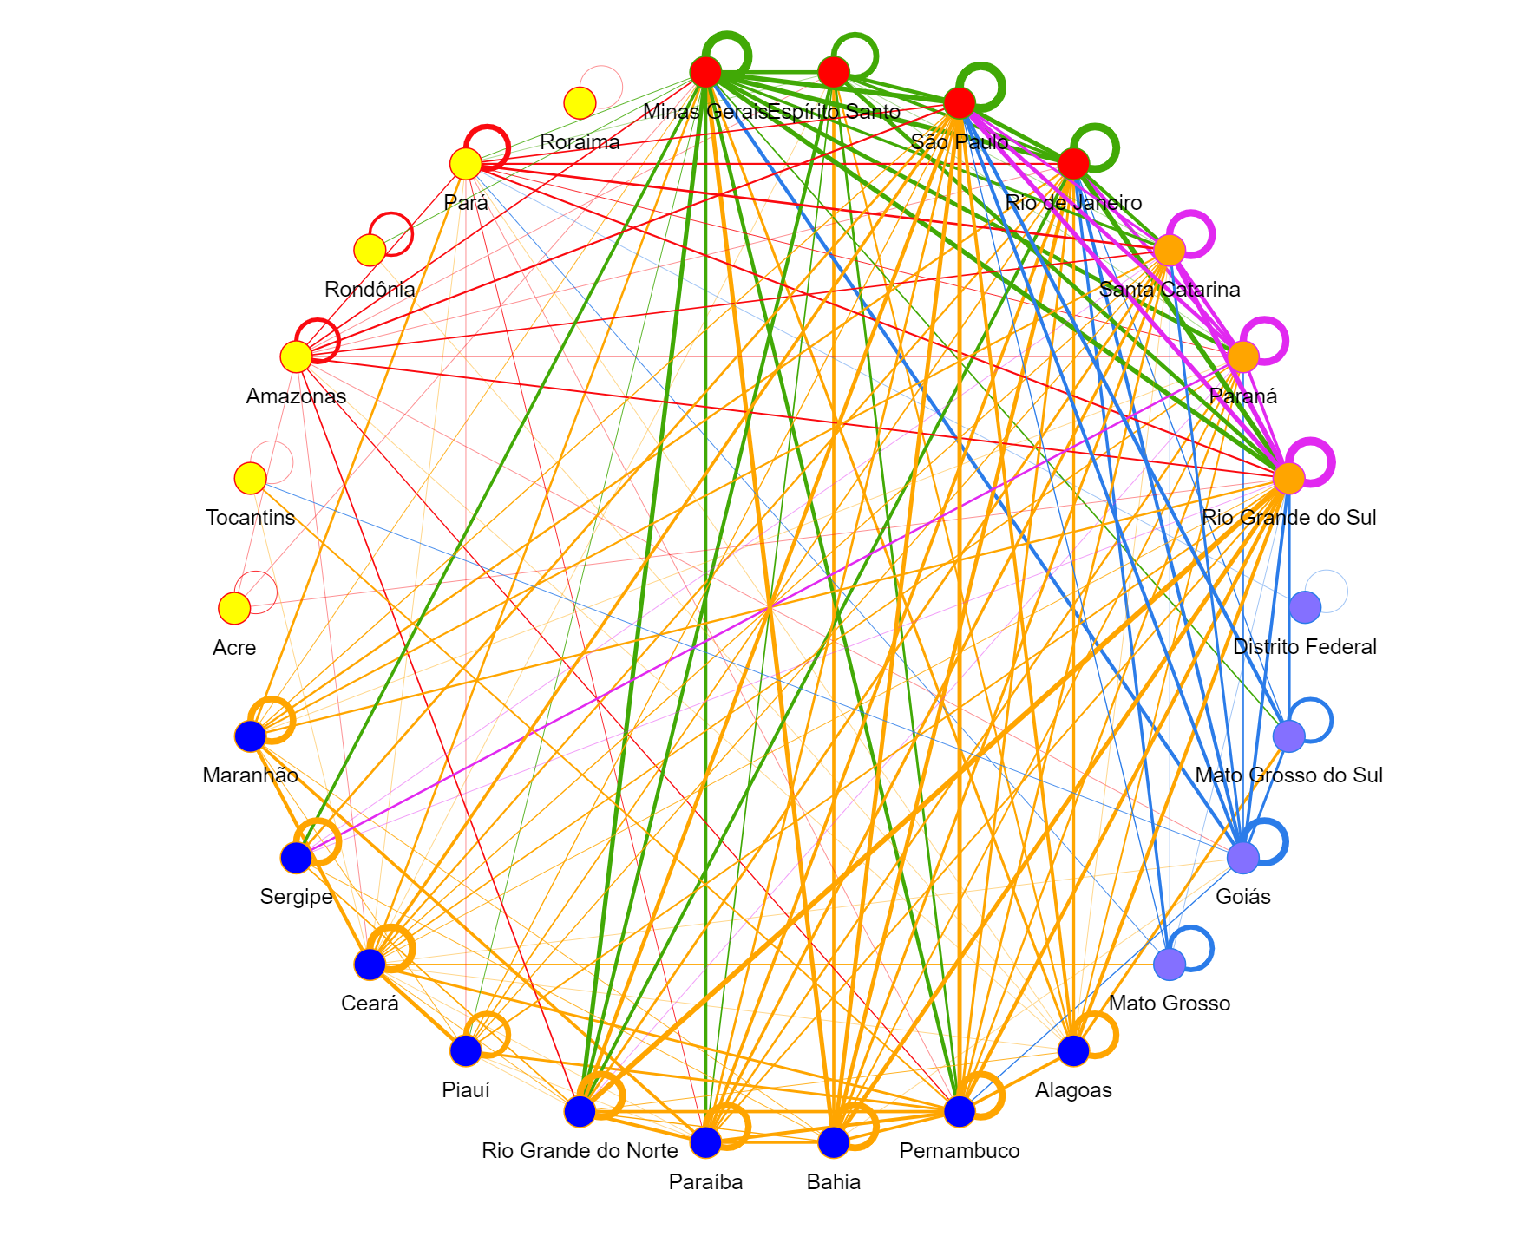
\includegraphics[width=0.35\textwidth]{Imagens/rede-2013.pdf} \\
		2011 & 2012 & 2013\\[6pt]
		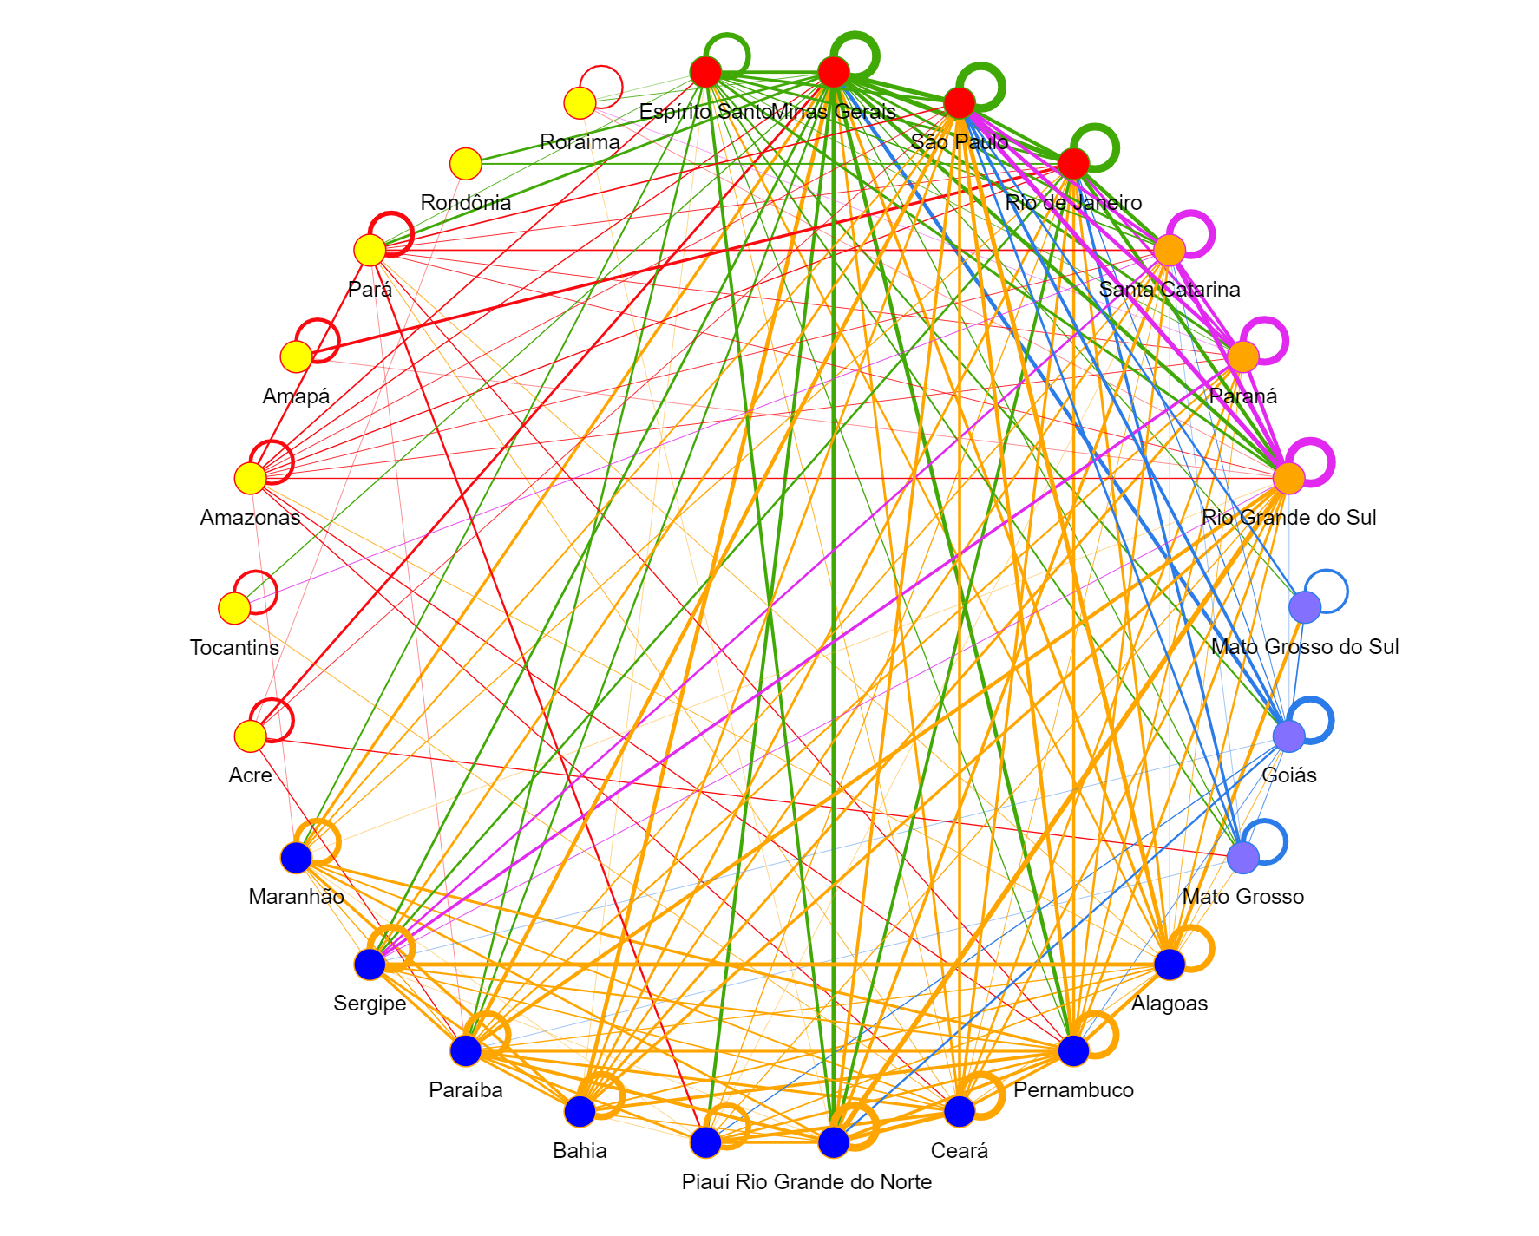
\includegraphics[width=0.35\textwidth]{Imagens/rede-2014.pdf} &
		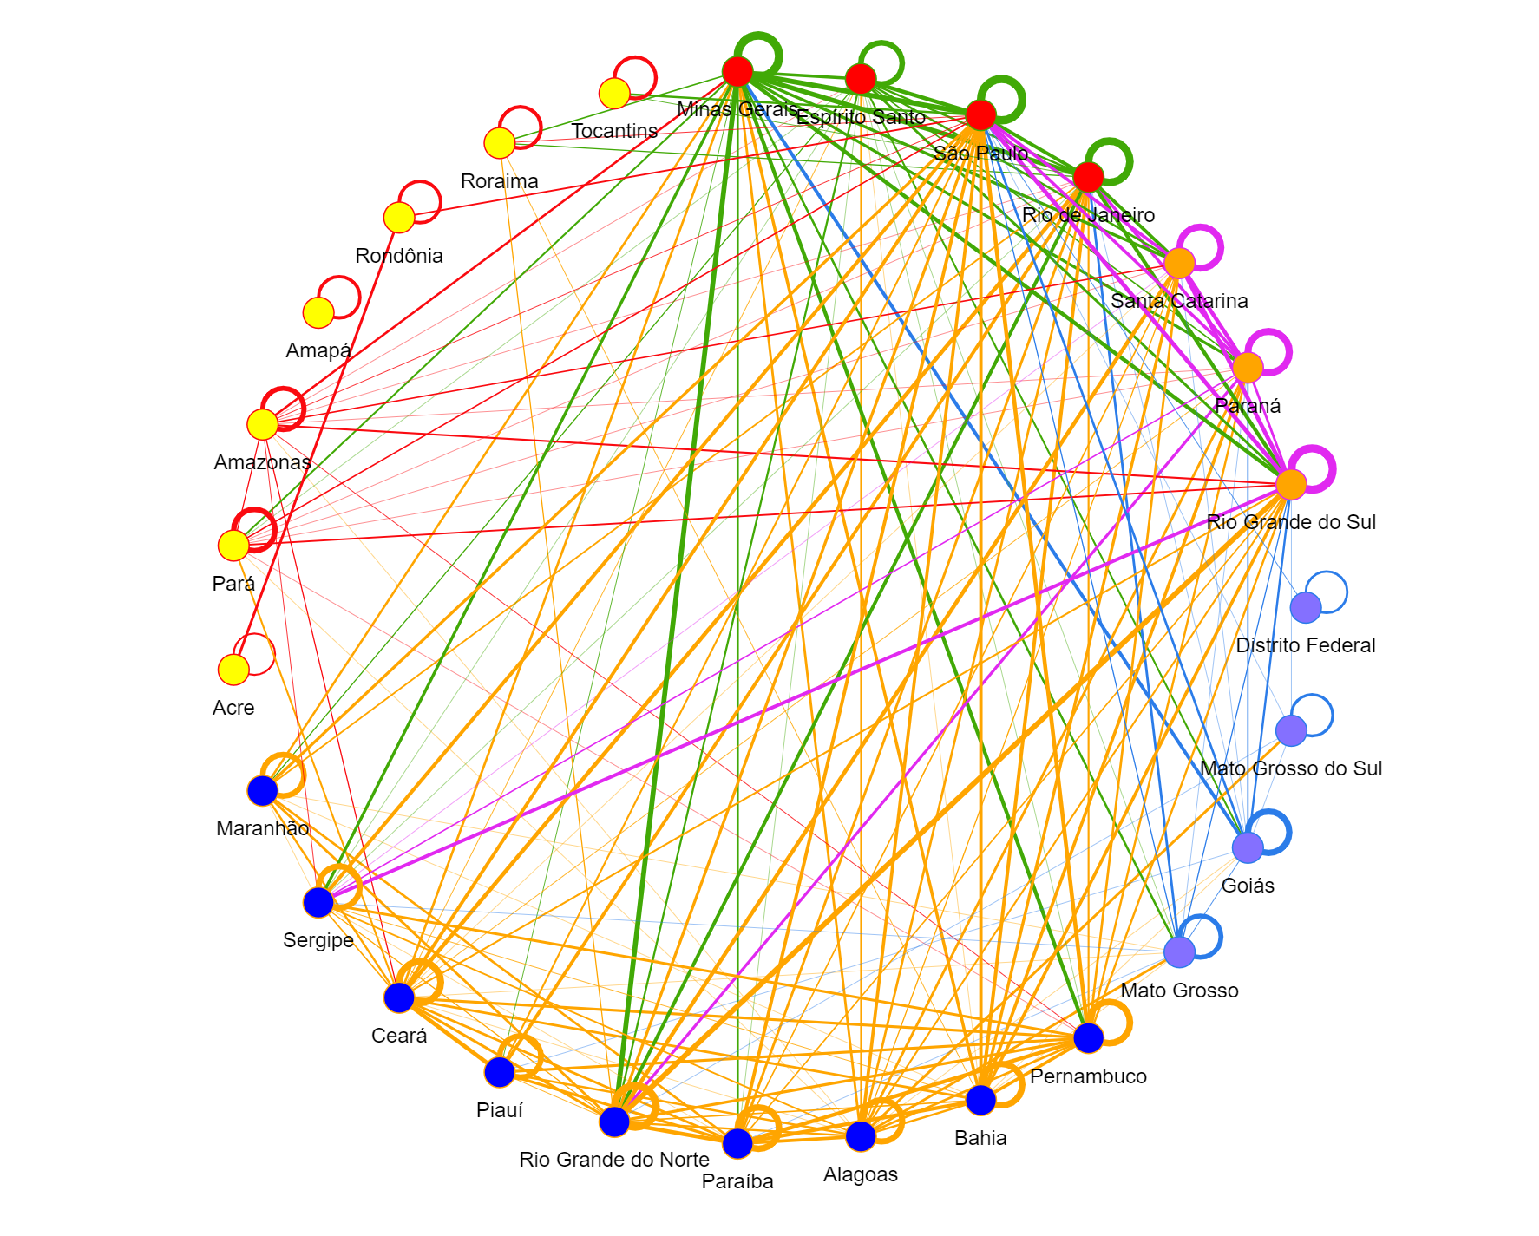
\includegraphics[width=0.35\textwidth]{Imagens/rede-2015.pdf} &
		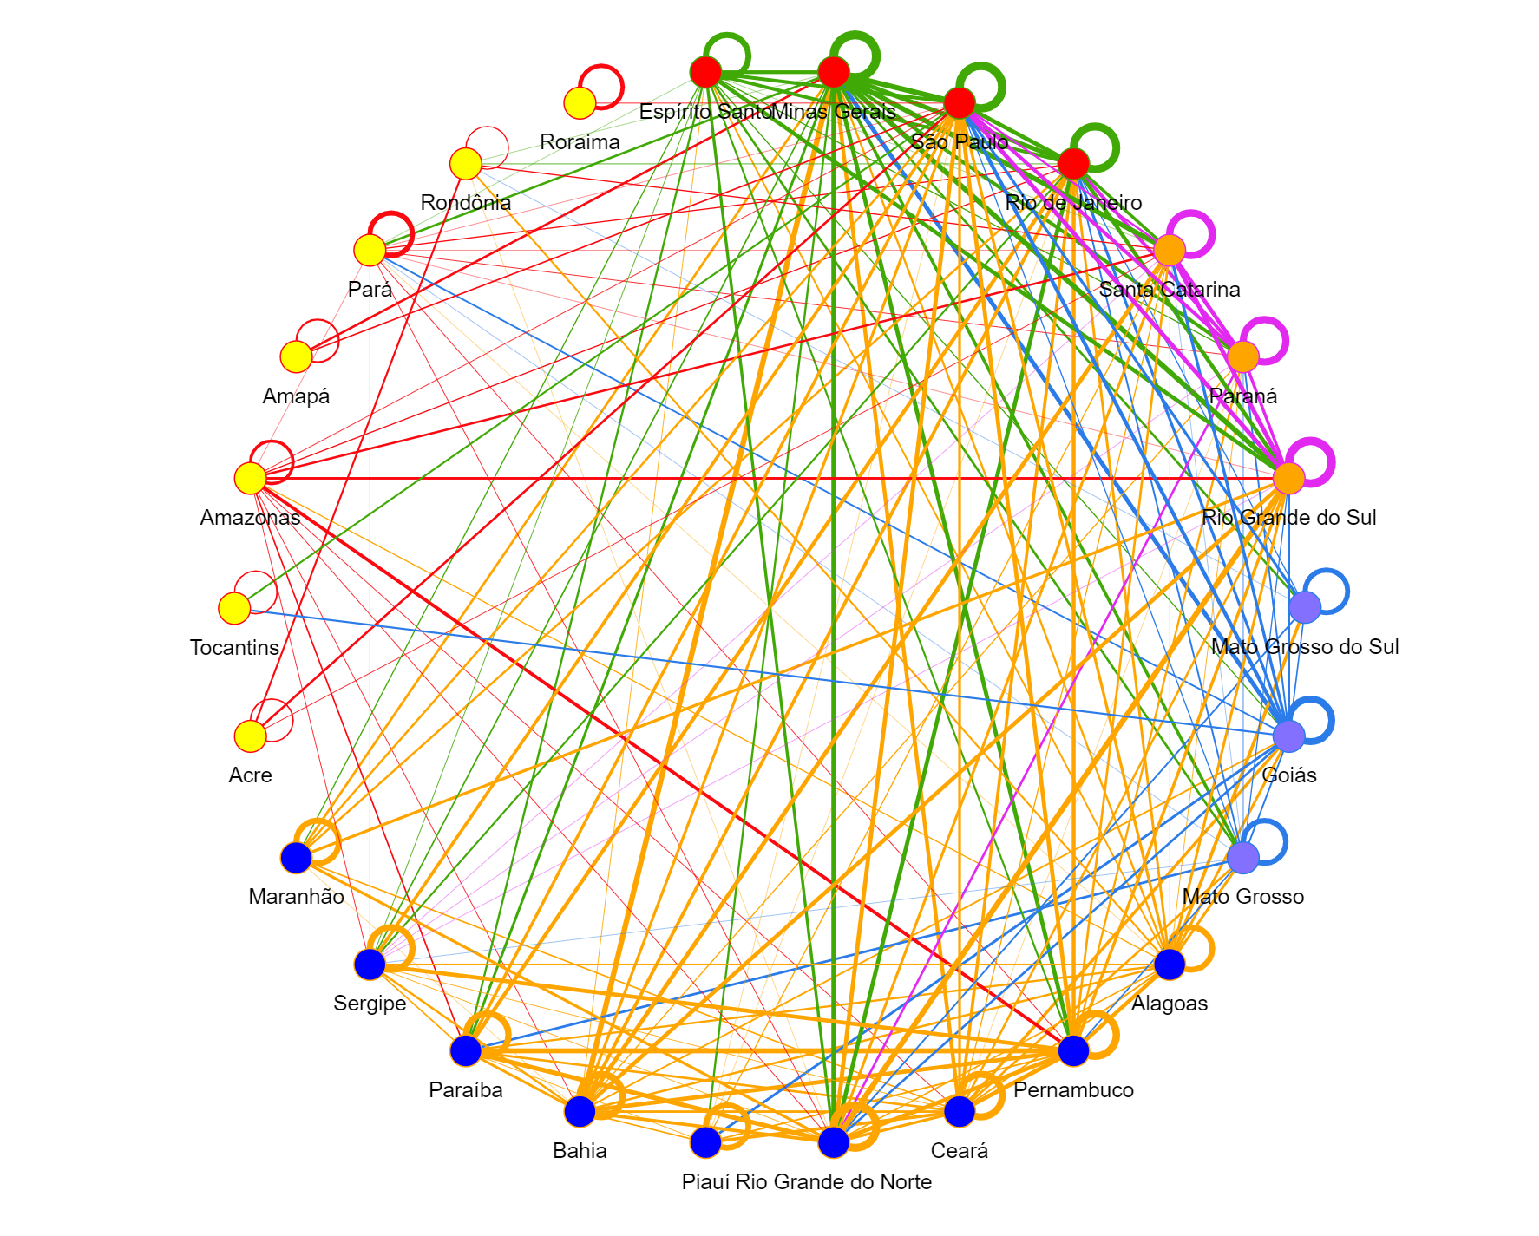
\includegraphics[width=0.35\textwidth]{Imagens/rede-2016.pdf} \\
		2014 & 2015 & 2016\\[6pt]  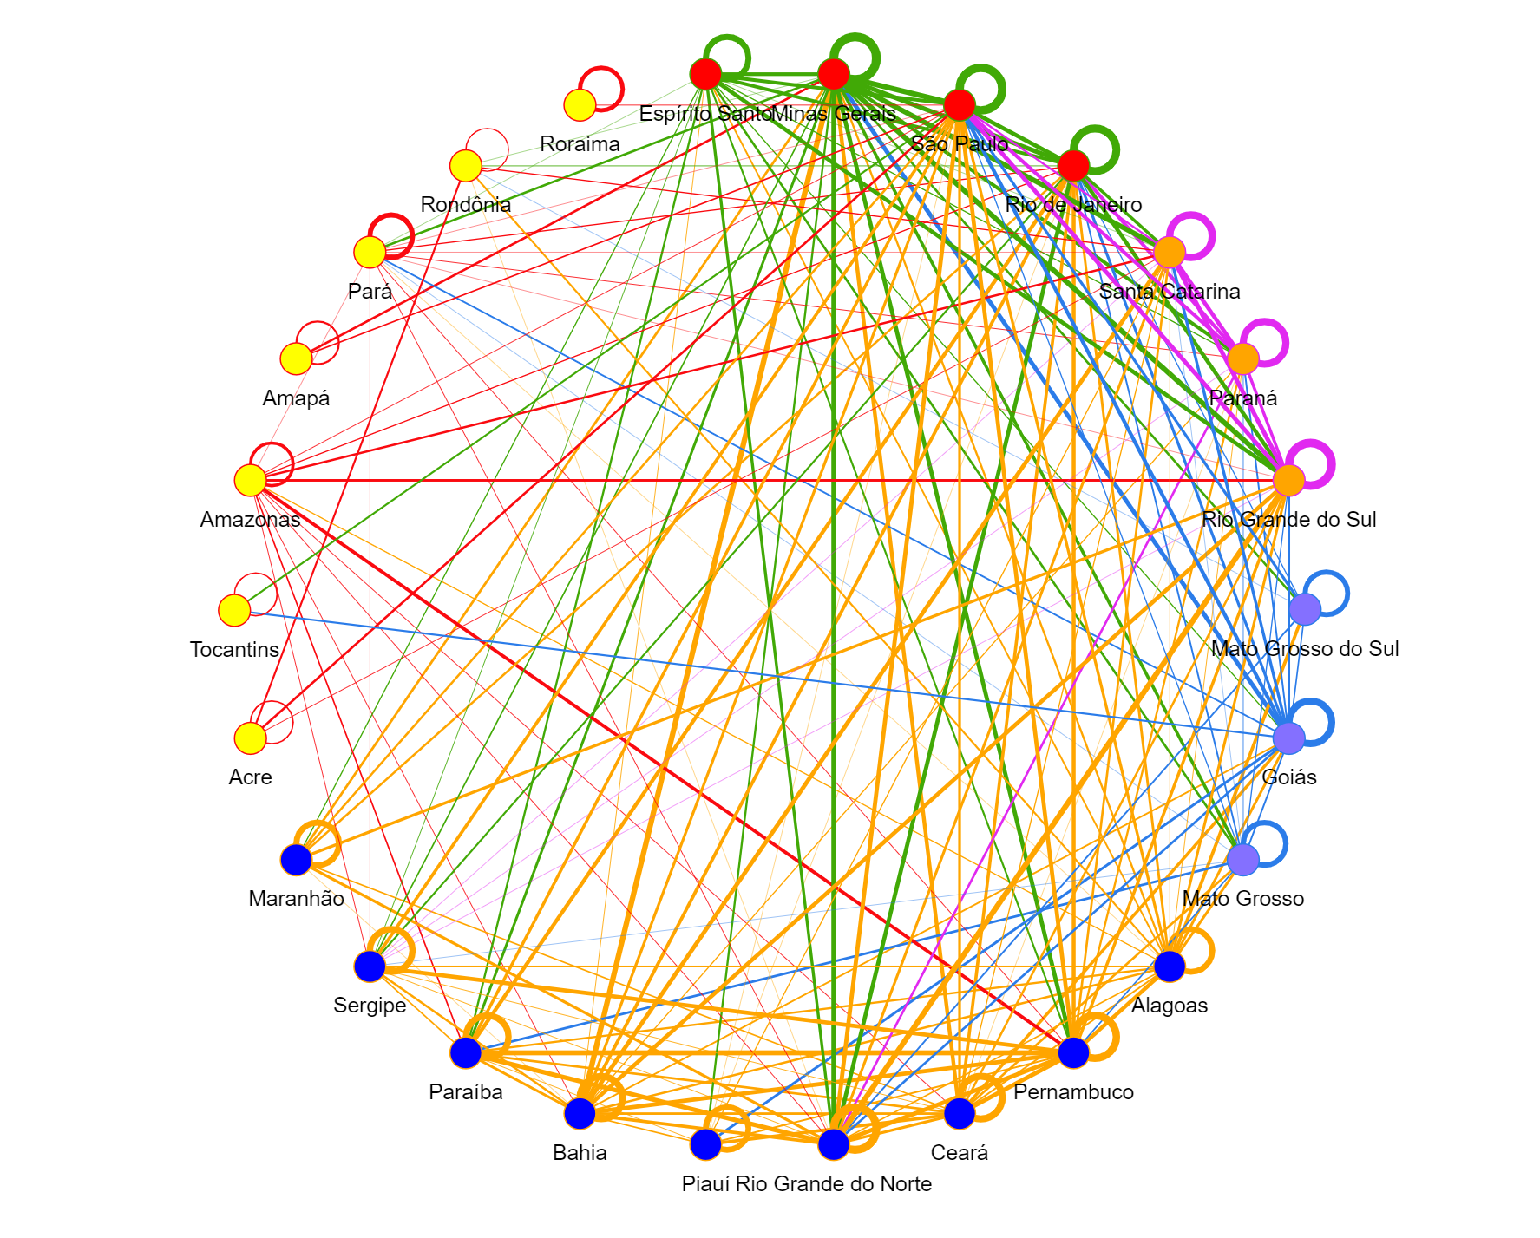
\includegraphics[width=0.35\textwidth]{Imagens/rede-2017.pdf} & & \\
		2017 & & \\
	\end{tabular}
	\caption{Redes de Coautoria Universidades Federal do Brasil (\textit{Health Sciences})}
	\label{rede-br-health}
\end{figure}

\subsubsection{Rede de Coautoria Brasil - Vértice Focal Alagoas}

A seguir são apresentadas as redes de coautoria utilizando o vértice focal Alagoas, e então observando as conexões realizadas com os demais vértices da rede (UF). Visualmente é possível notar o crescimento pelo número de novas conexões.


\begin{figure}[H]
	\begin{tabular}{ccc}
		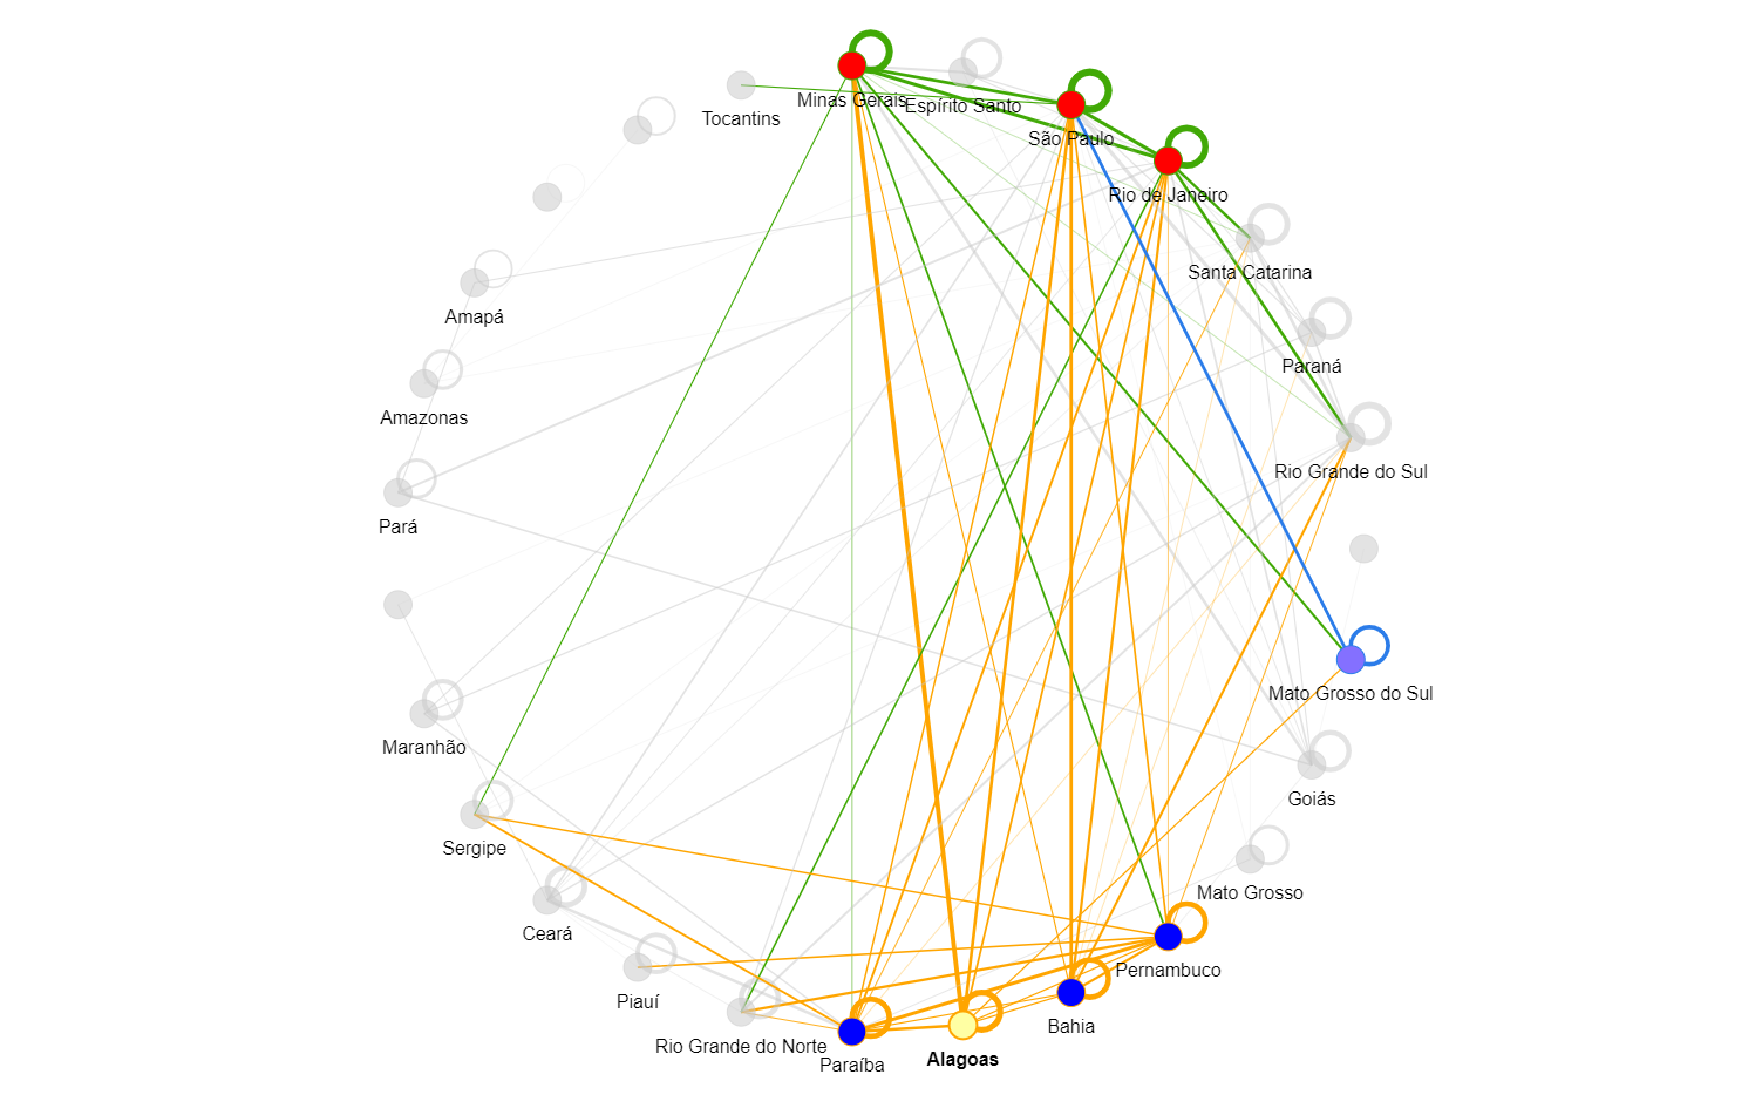
\includegraphics[width=0.38\textwidth]{Imagens/rede-al-2008.pdf} &   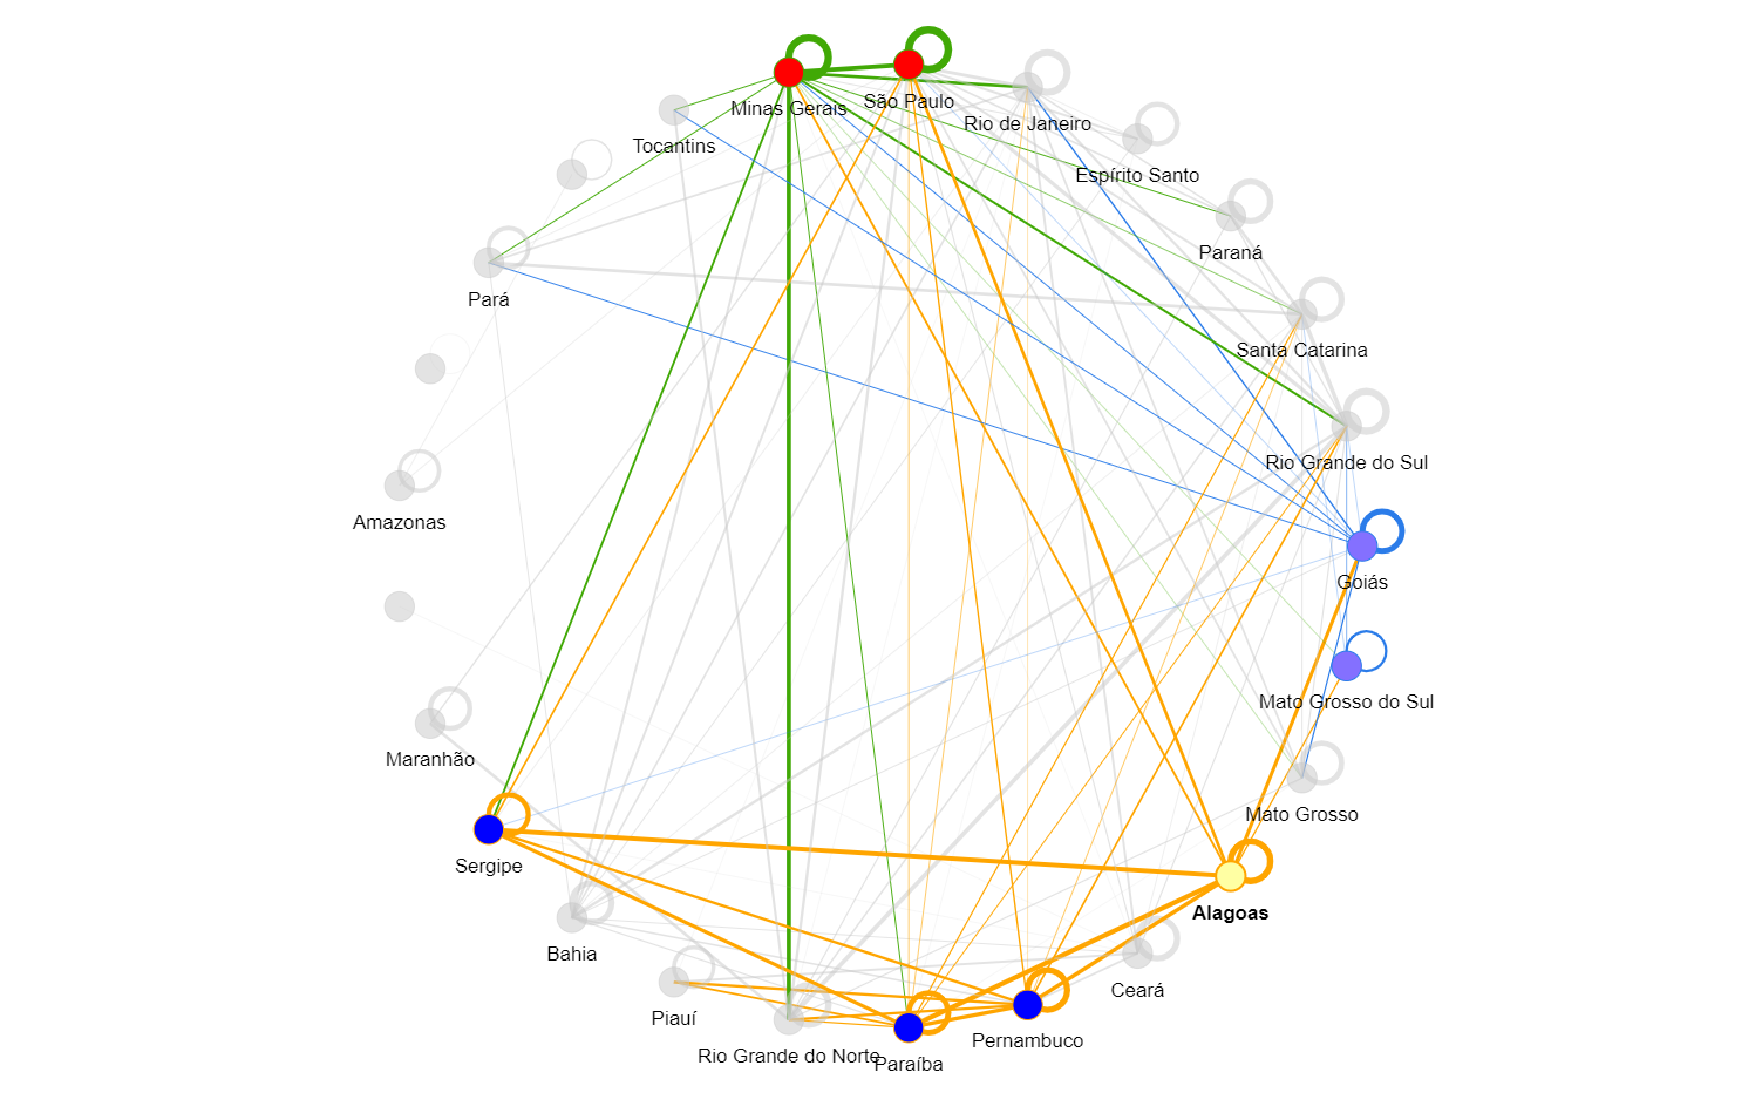
\includegraphics[width=0.38\textwidth]{Imagens/rede-al-2009.pdf} &
		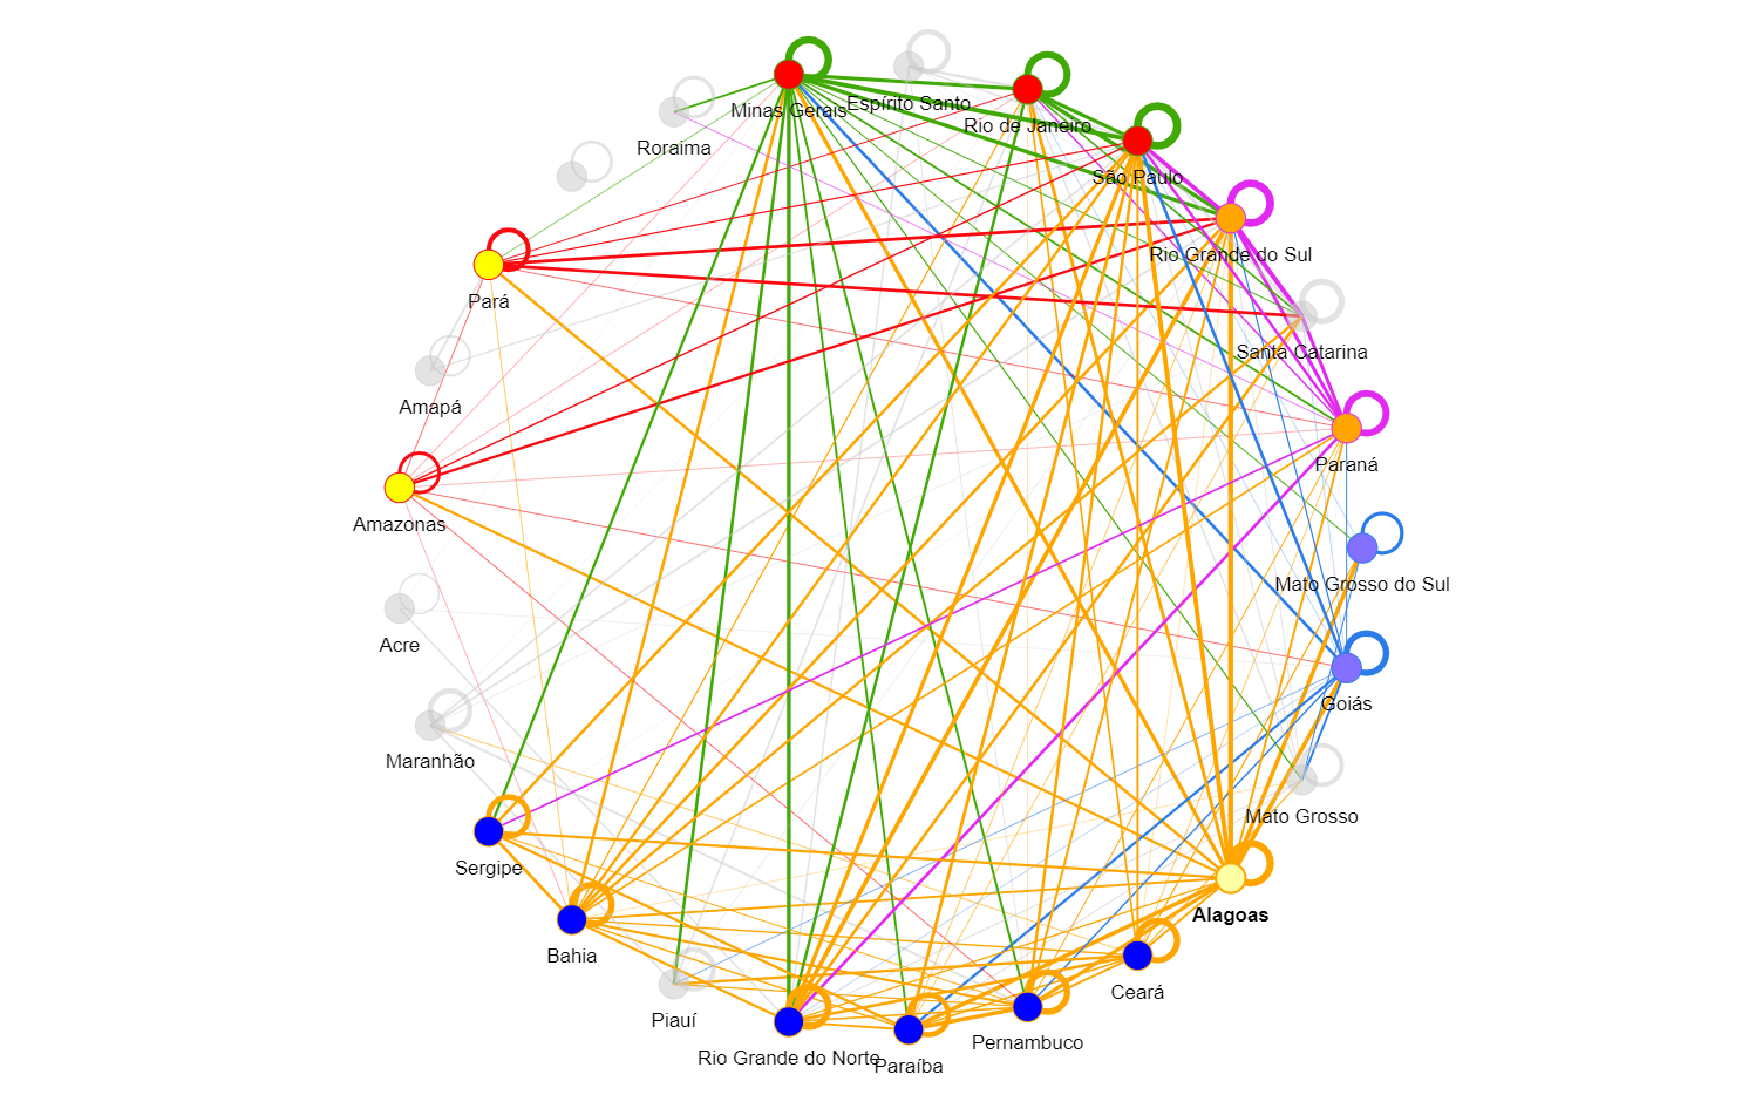
\includegraphics[width=0.38\textwidth]{Imagens/rede-al-2010.pdf}\\
		2008 & 2009 & 2010\\[6pt] 
		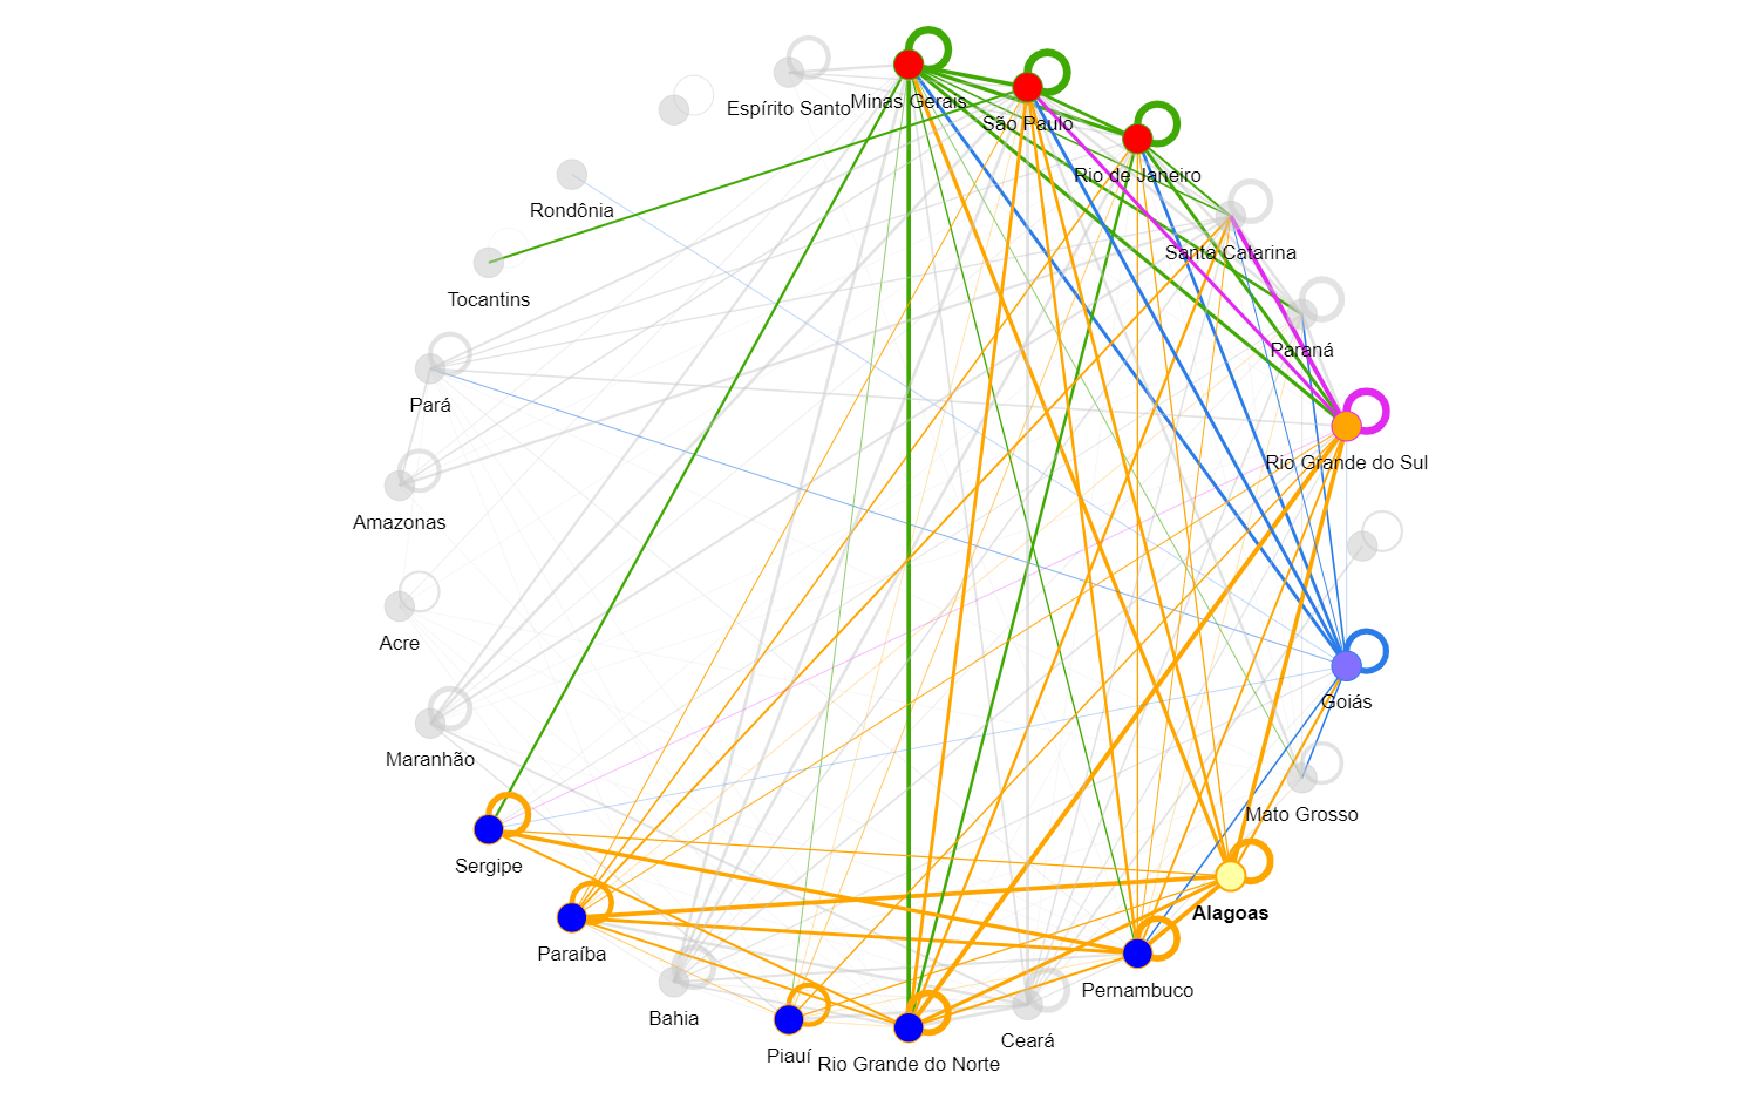
\includegraphics[width=0.38\textwidth]{Imagens/rede-al-2011.pdf} &
		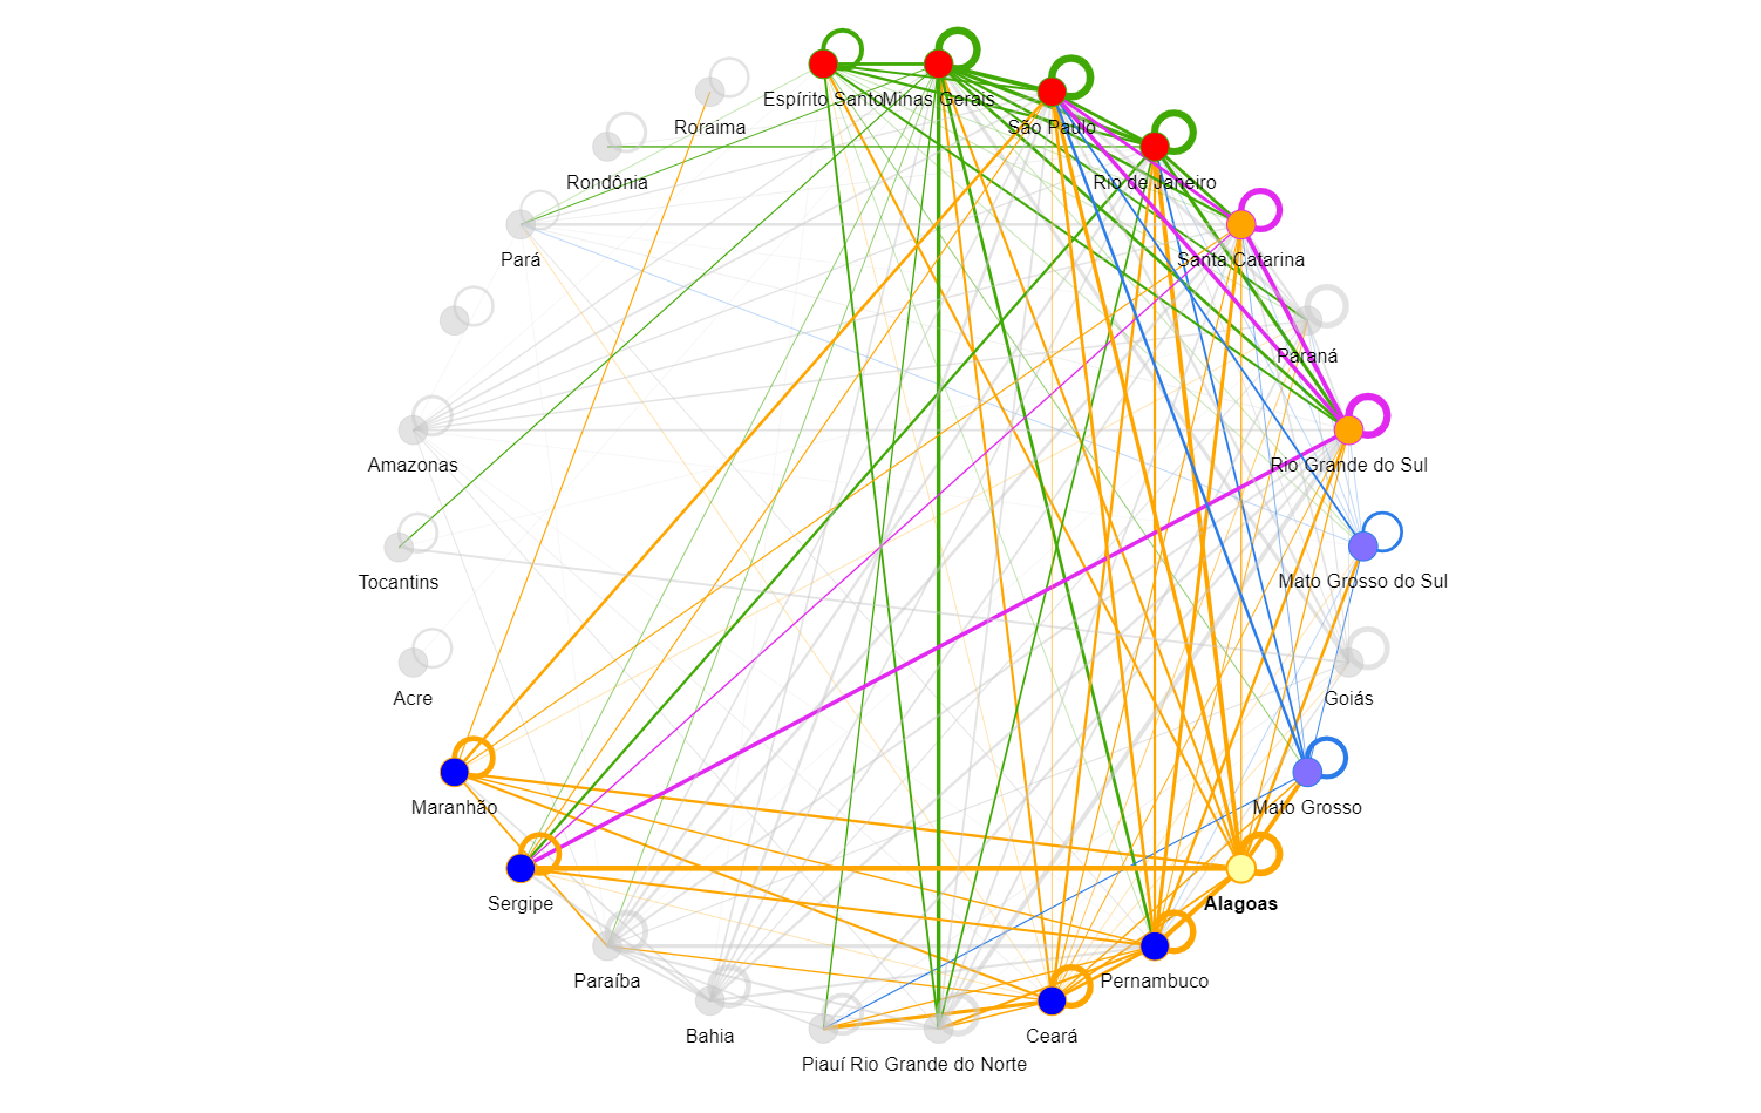
\includegraphics[width=0.38\textwidth]{Imagens/rede-al-2012.pdf} &   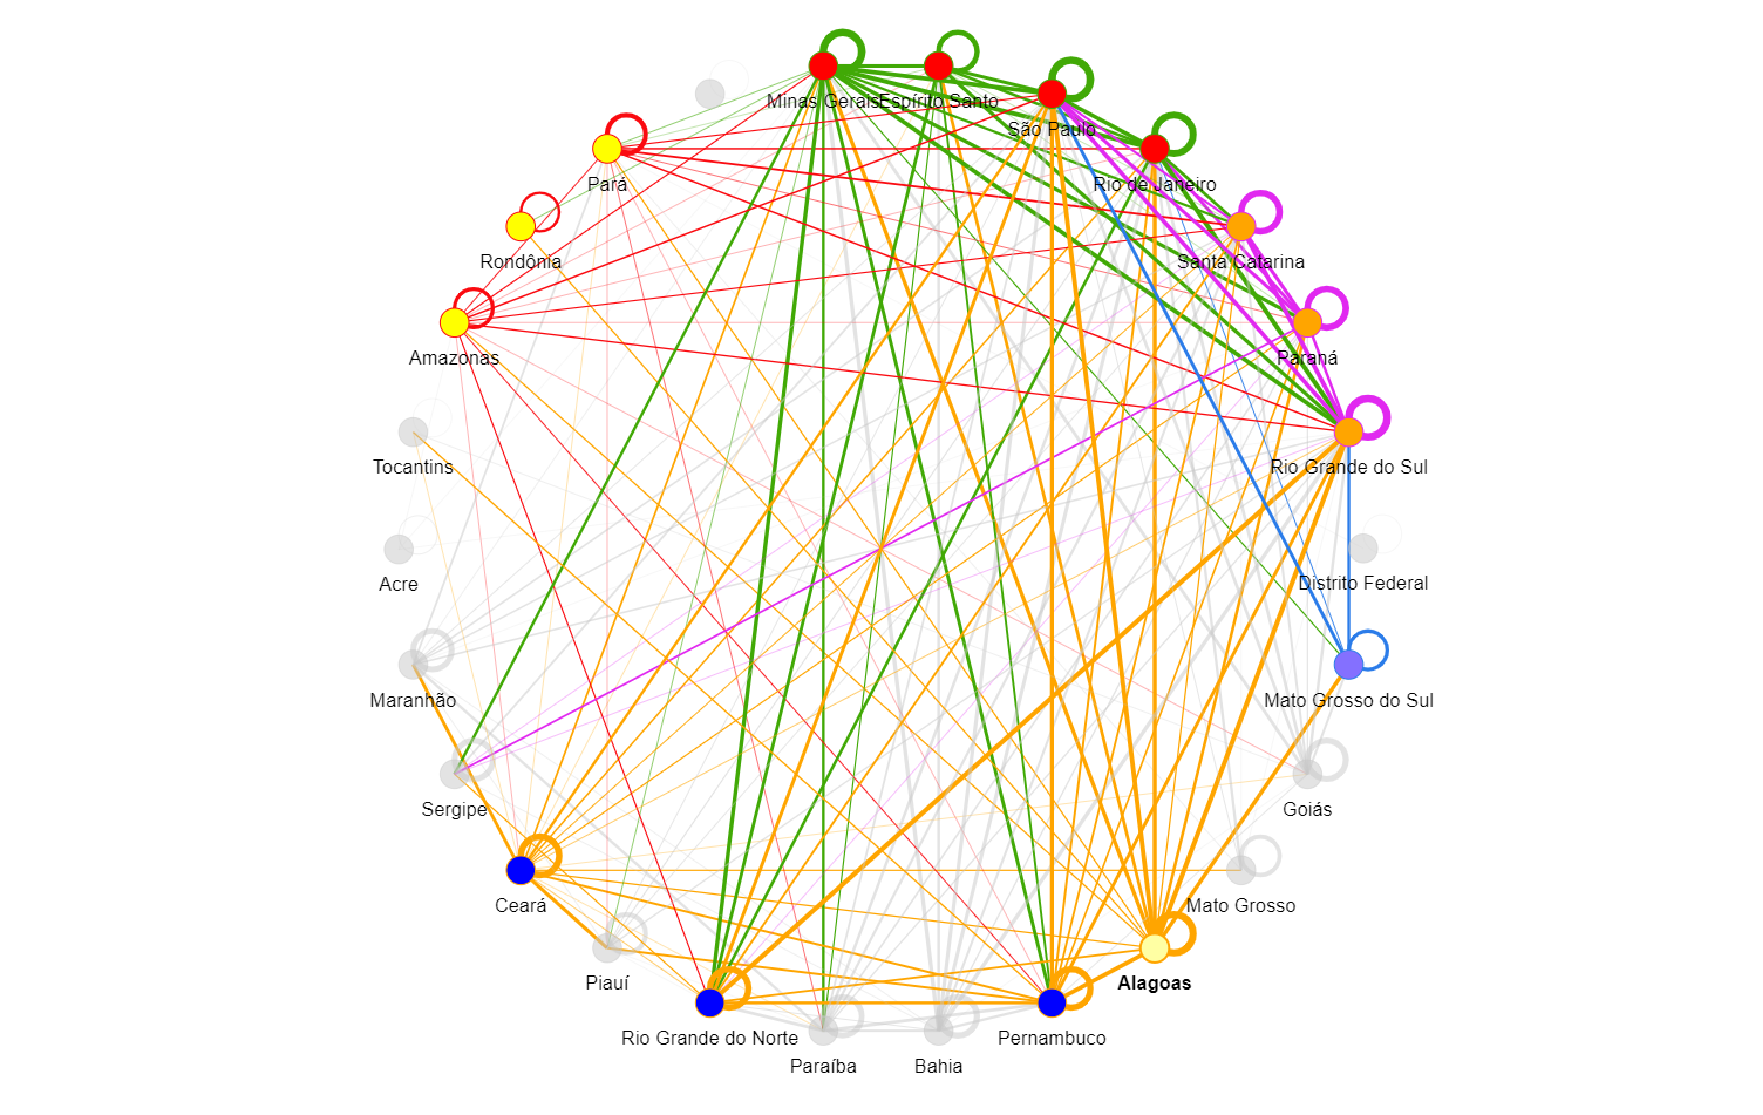
\includegraphics[width=0.38\textwidth]{Imagens/rede-al-2013.pdf} \\
		2011 & 2012 & 2013\\[6pt]
		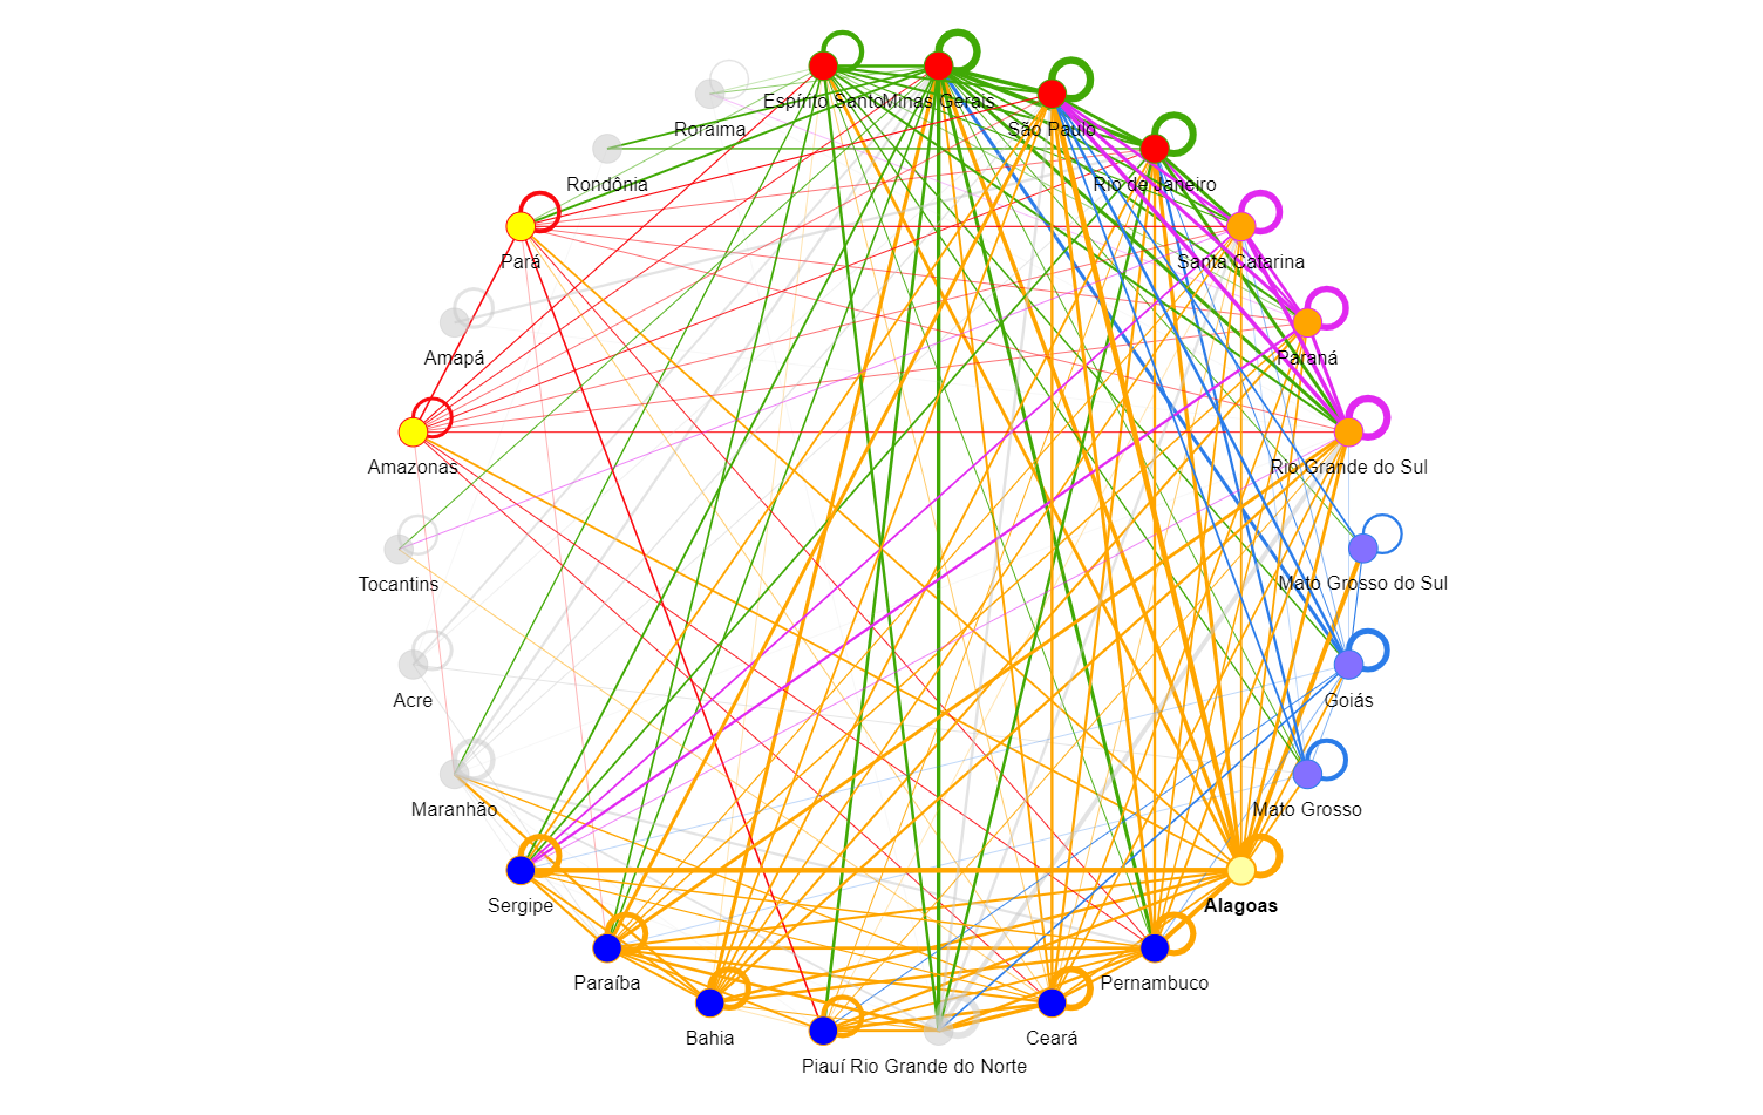
\includegraphics[width=0.38\textwidth]{Imagens/rede-al-2014.pdf} &
		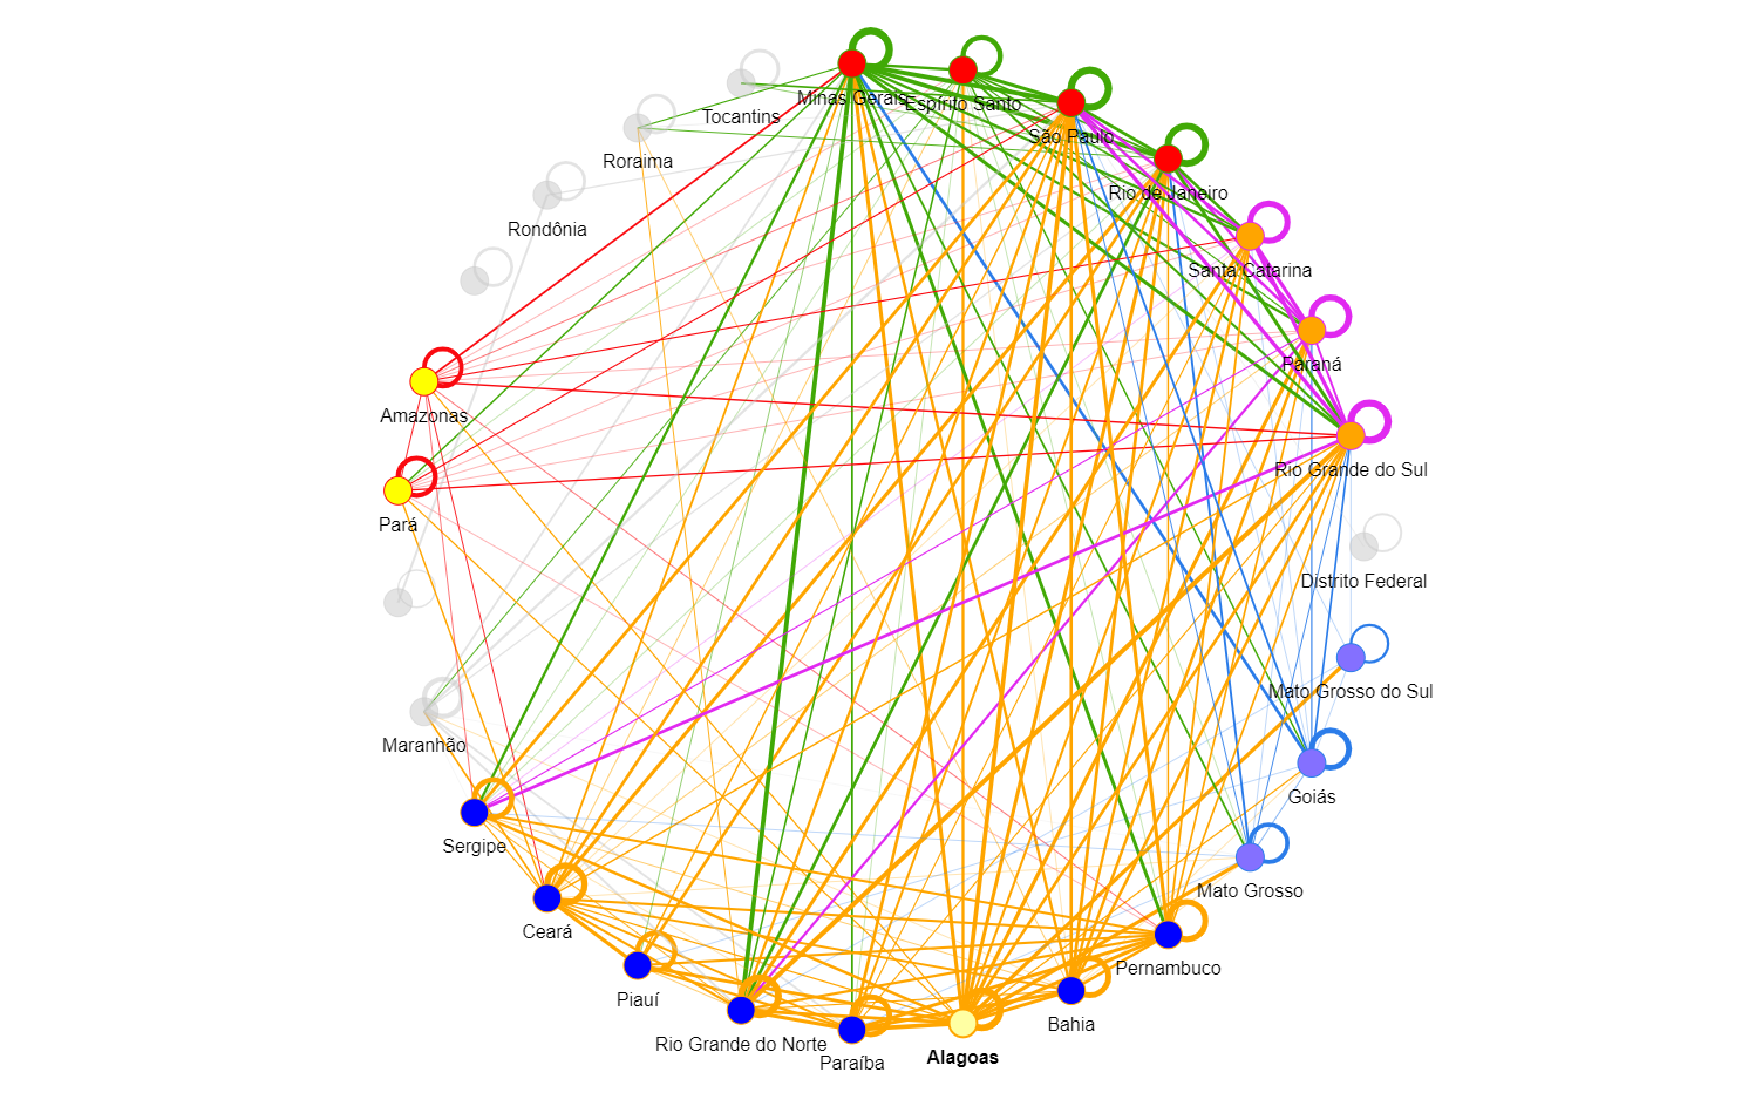
\includegraphics[width=0.38\textwidth]{Imagens/rede-al-2015.pdf} &
		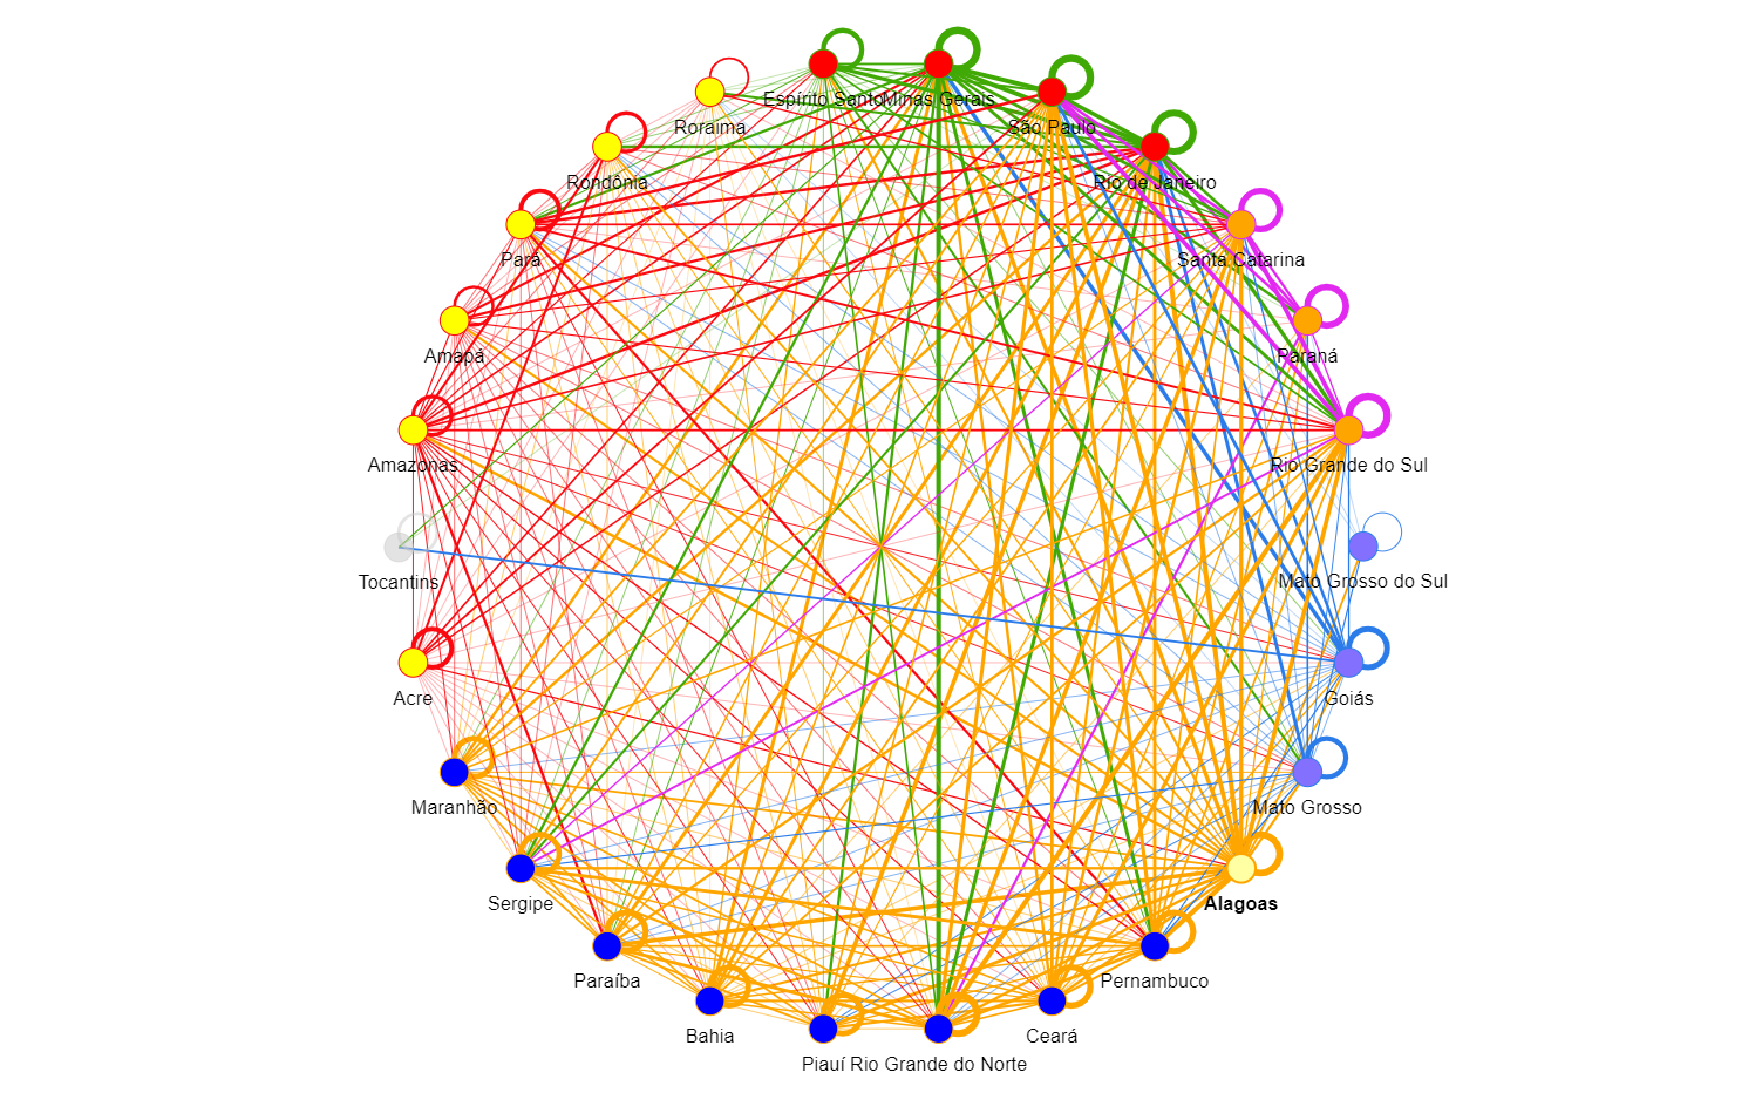
\includegraphics[width=0.38\textwidth]{Imagens/rede-al-2016.pdf} \\
		2014 & 2015 & 2016\\[6pt]  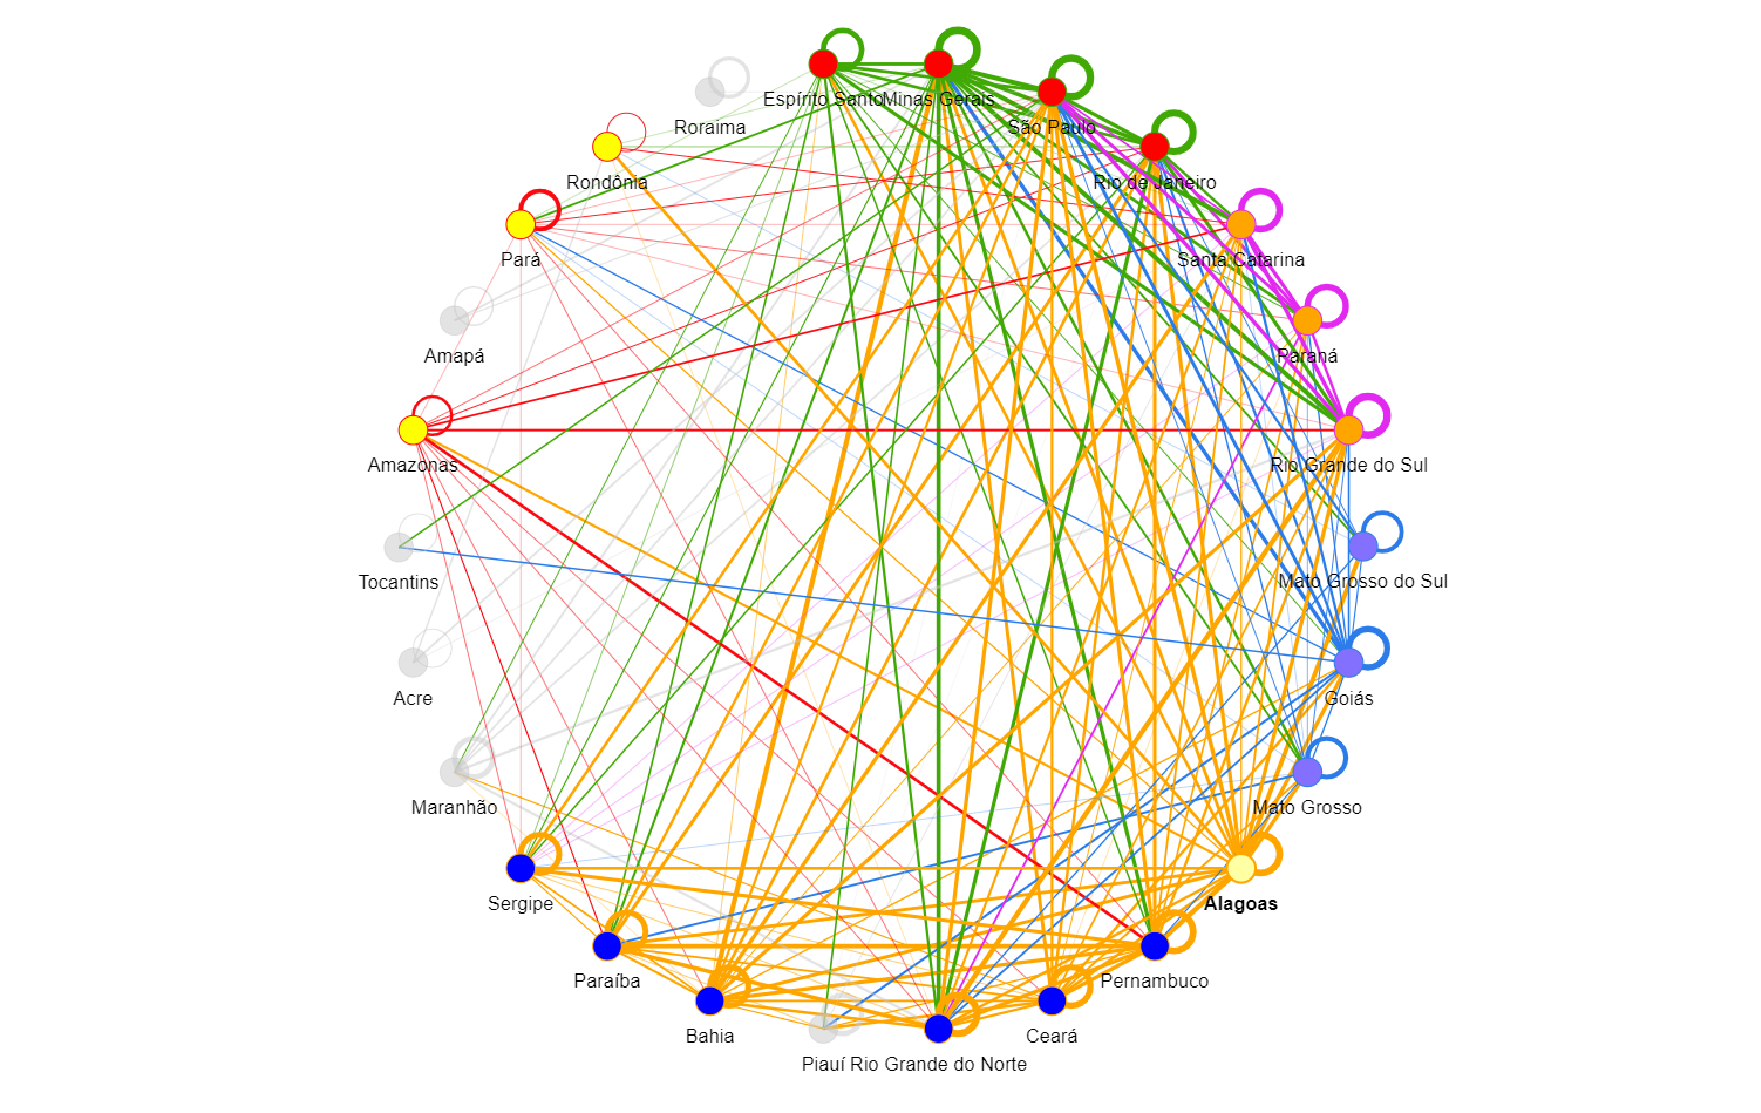
\includegraphics[width=0.38\textwidth]{Imagens/rede-al-2017.pdf} & & \\
		2017 & & \\
	\end{tabular}
	\caption{Redes de Coautoria da Universidade Federal de Alagoas}
\end{figure}


%\begin{figure}[H]
%\centering
%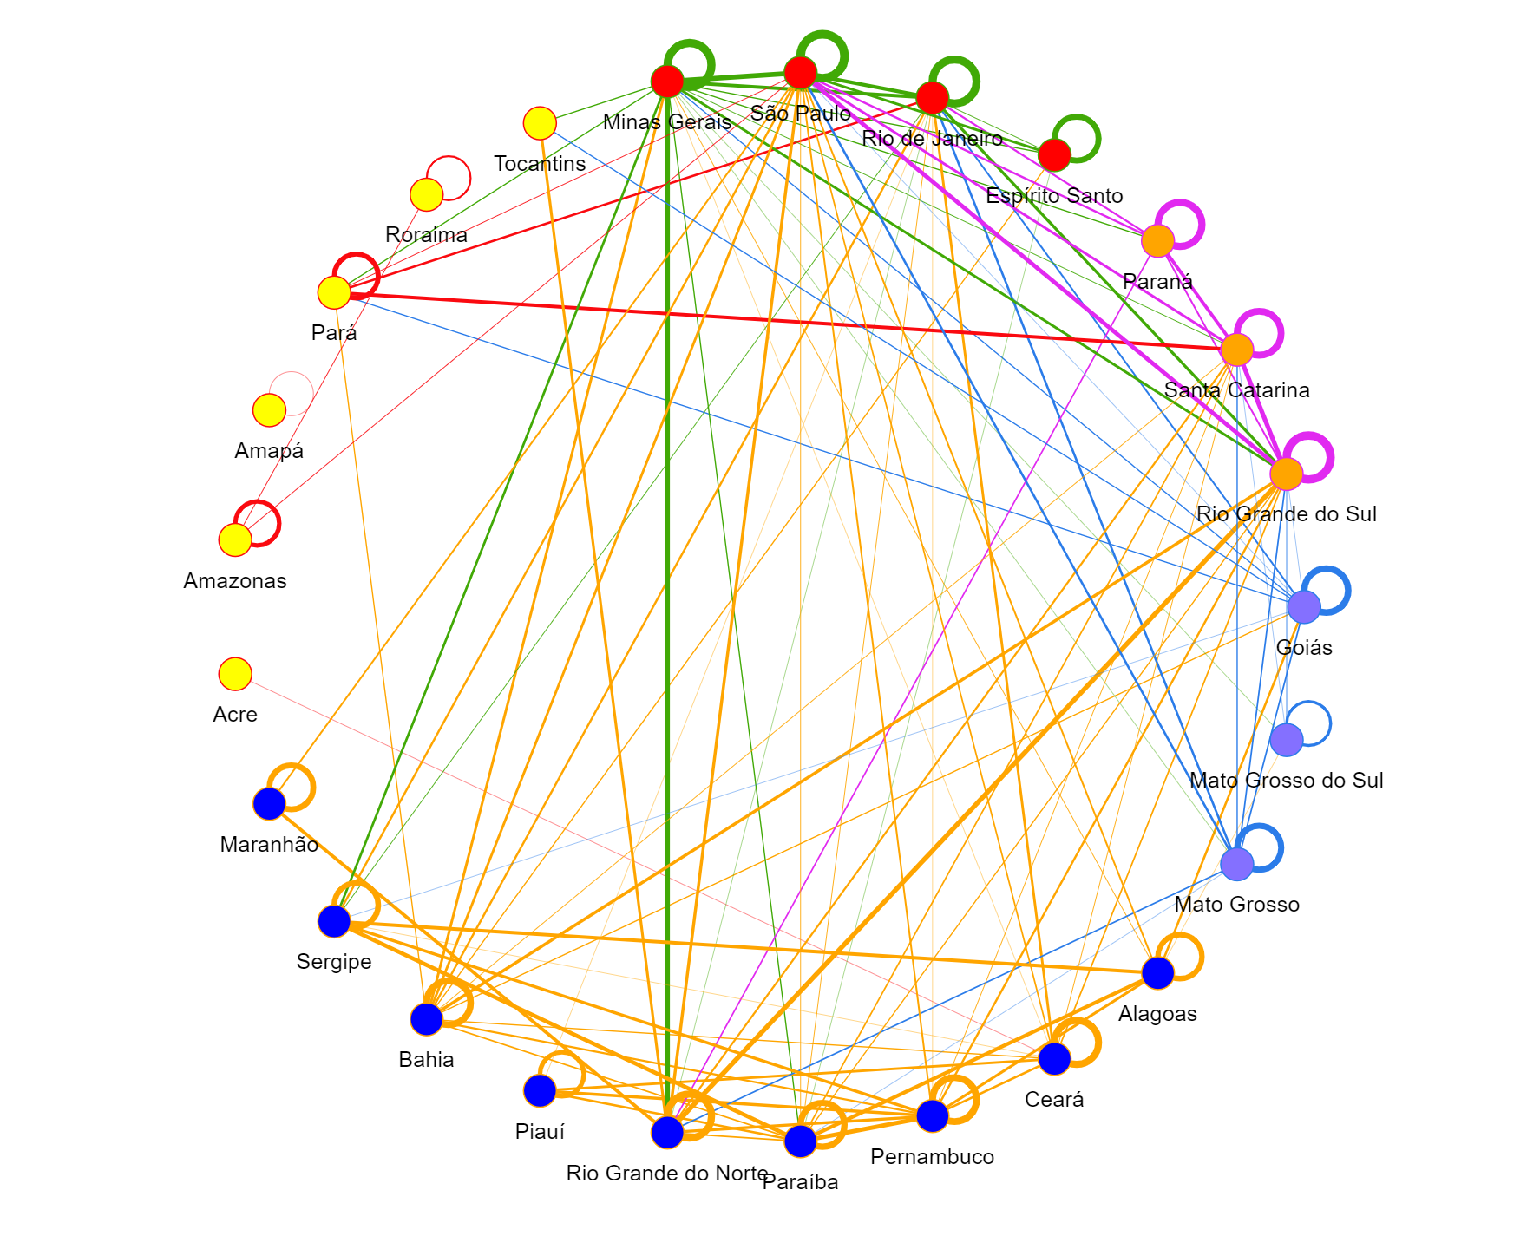
\includegraphics[scale=0.6]{Imagens/rede-2009.pdf}
%\caption{Rede de Coautoria das Universidades Federais do Brasil - 2009}
%\label{Rede de Coautoria - UF BR 2009}
%\end{figure}

%\begin{figure}[H]
%\centering
%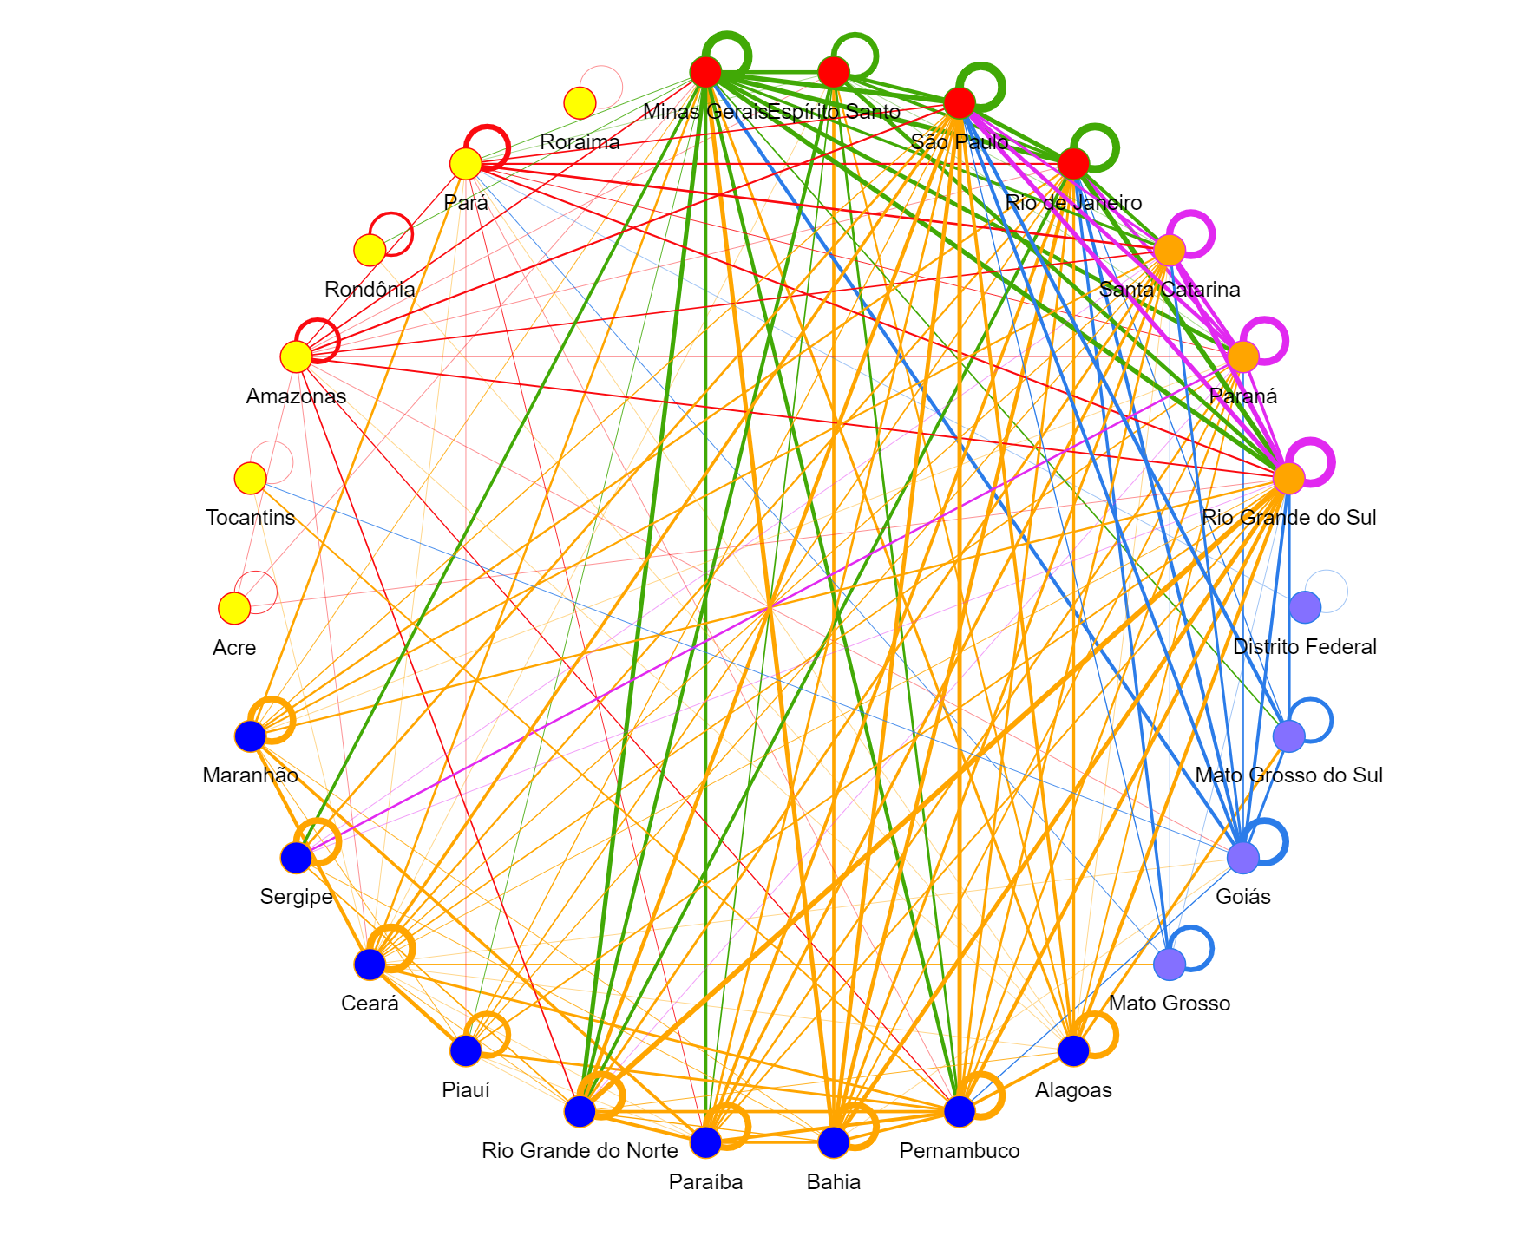
\includegraphics[scale=0.6]{Imagens/rede-2013.pdf}
%\caption{Rede de Coautoria das Universidades Federais do Brasil - 2013}
%\label{Rede de Coautoria - UF BR 2013}
%\end{figure}

%\begin{figure}[H]
%\centering
%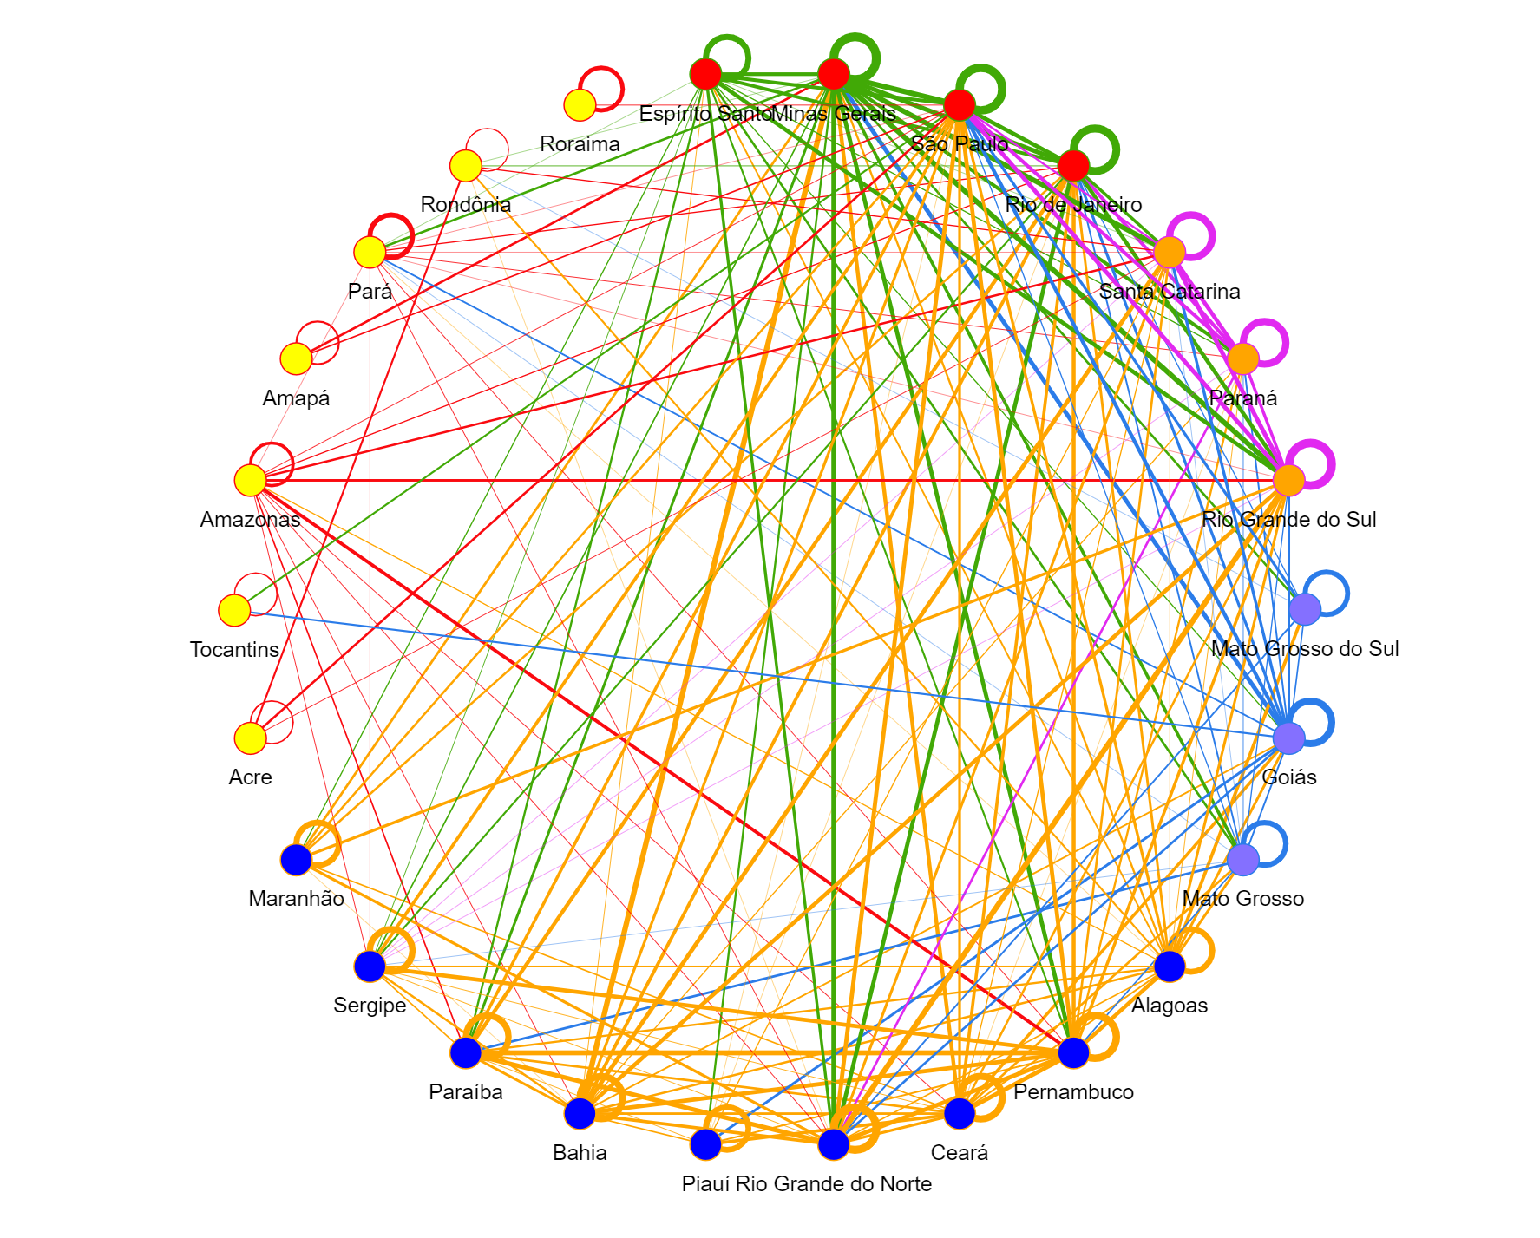
\includegraphics[scale=0.6]{Imagens/rede-2017.pdf}
%\caption{Rede de Coautoria das Universidades Federais do Brasil - 2007}
%\label{Rede de Coautoria - UF BR 2017}
%\end{figure}

\section{\textbf{Agricultural Sciences}}

\subsubsection{Rede de Coautoria das Universidade Federais do Brasil}

\begin{figure}[H]
	\begin{tabular}{ccc}
		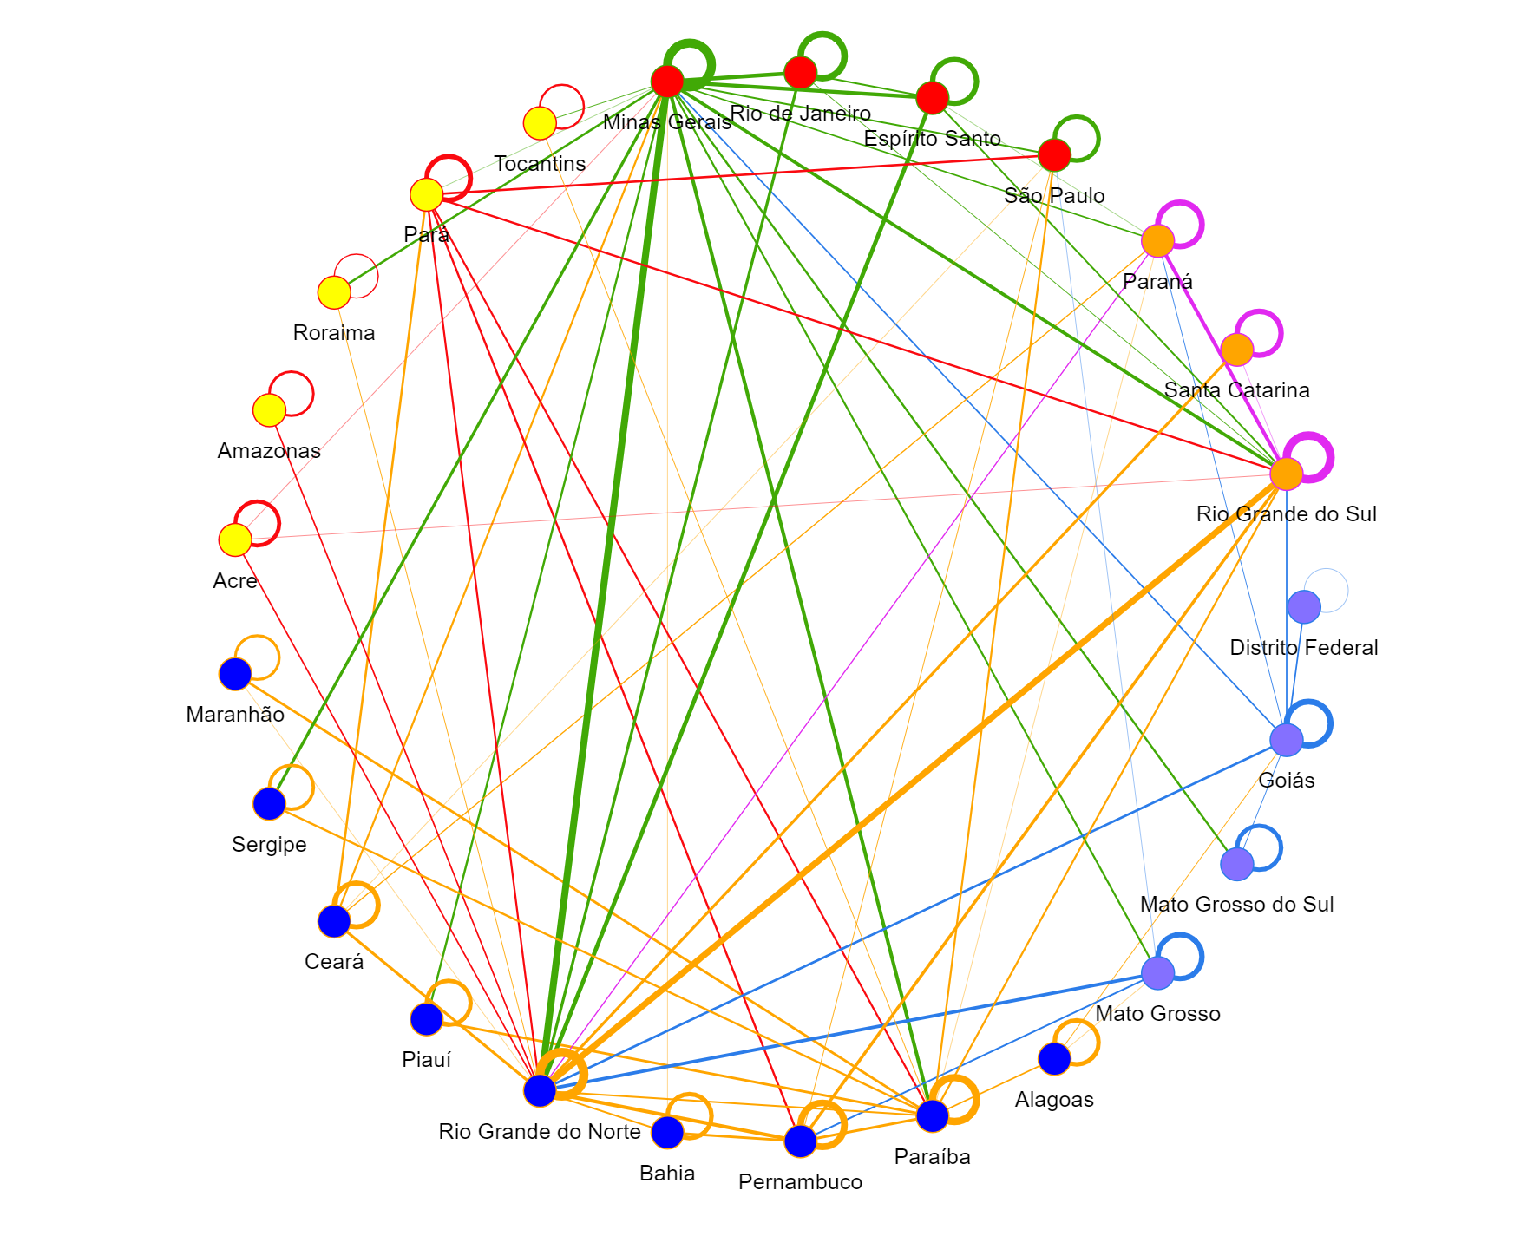
\includegraphics[width=0.35\textwidth]{Imagens/rede-agr-br-2008.pdf} &   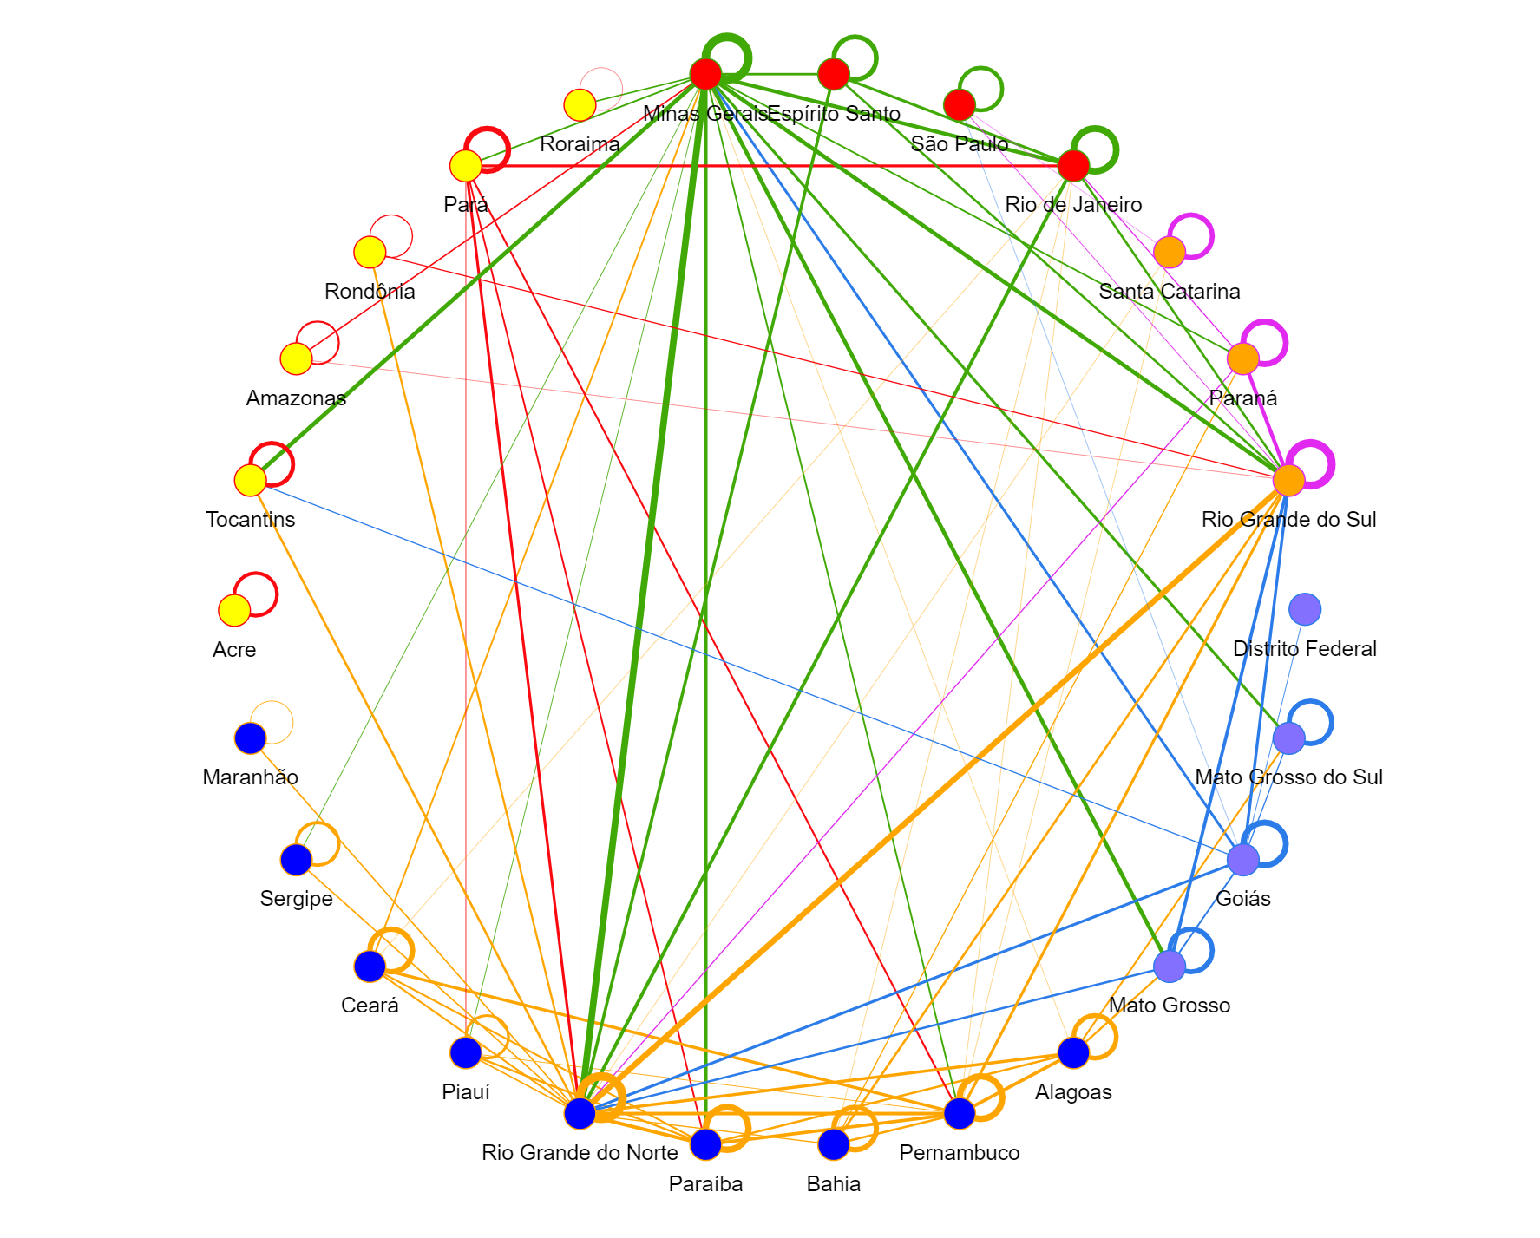
\includegraphics[width=0.35\textwidth]{Imagens/rede-agr-br-2009.pdf} &
		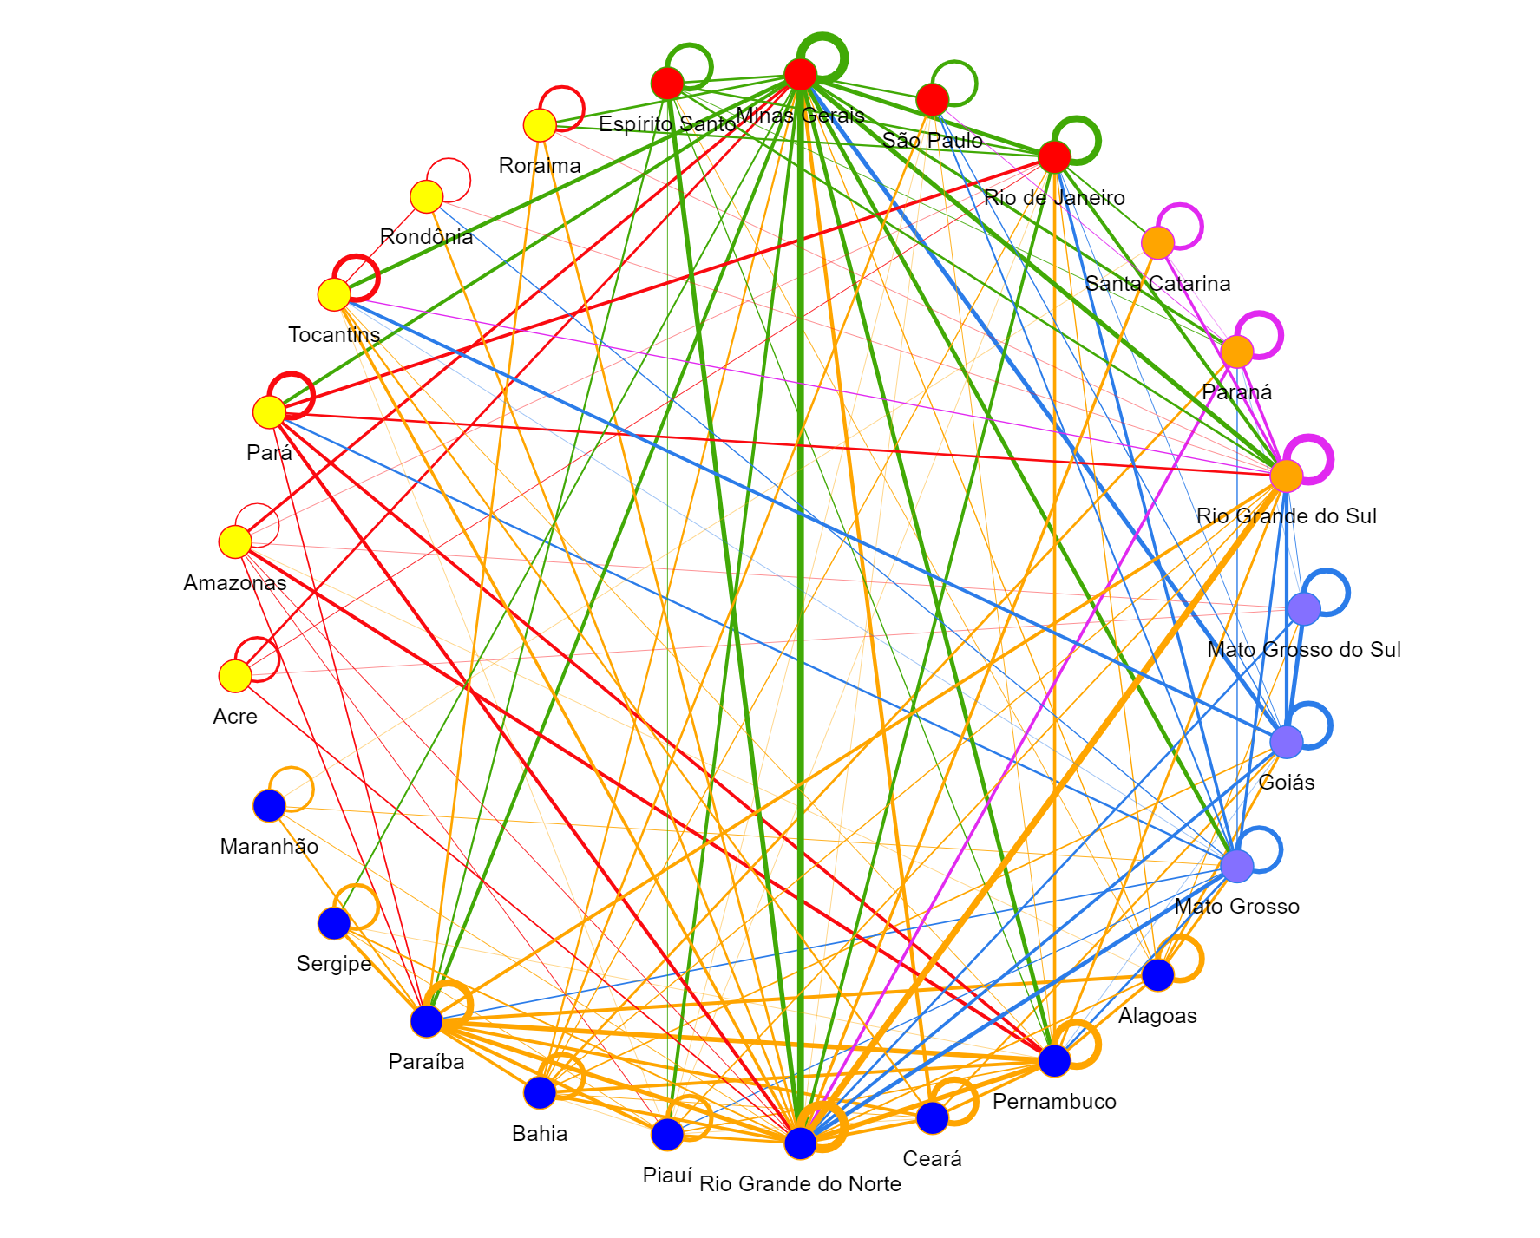
\includegraphics[width=0.35\textwidth]{Imagens/rede-agr-br-2010.pdf}\\
		2008 & 2009 & 2010\\[6pt] 
		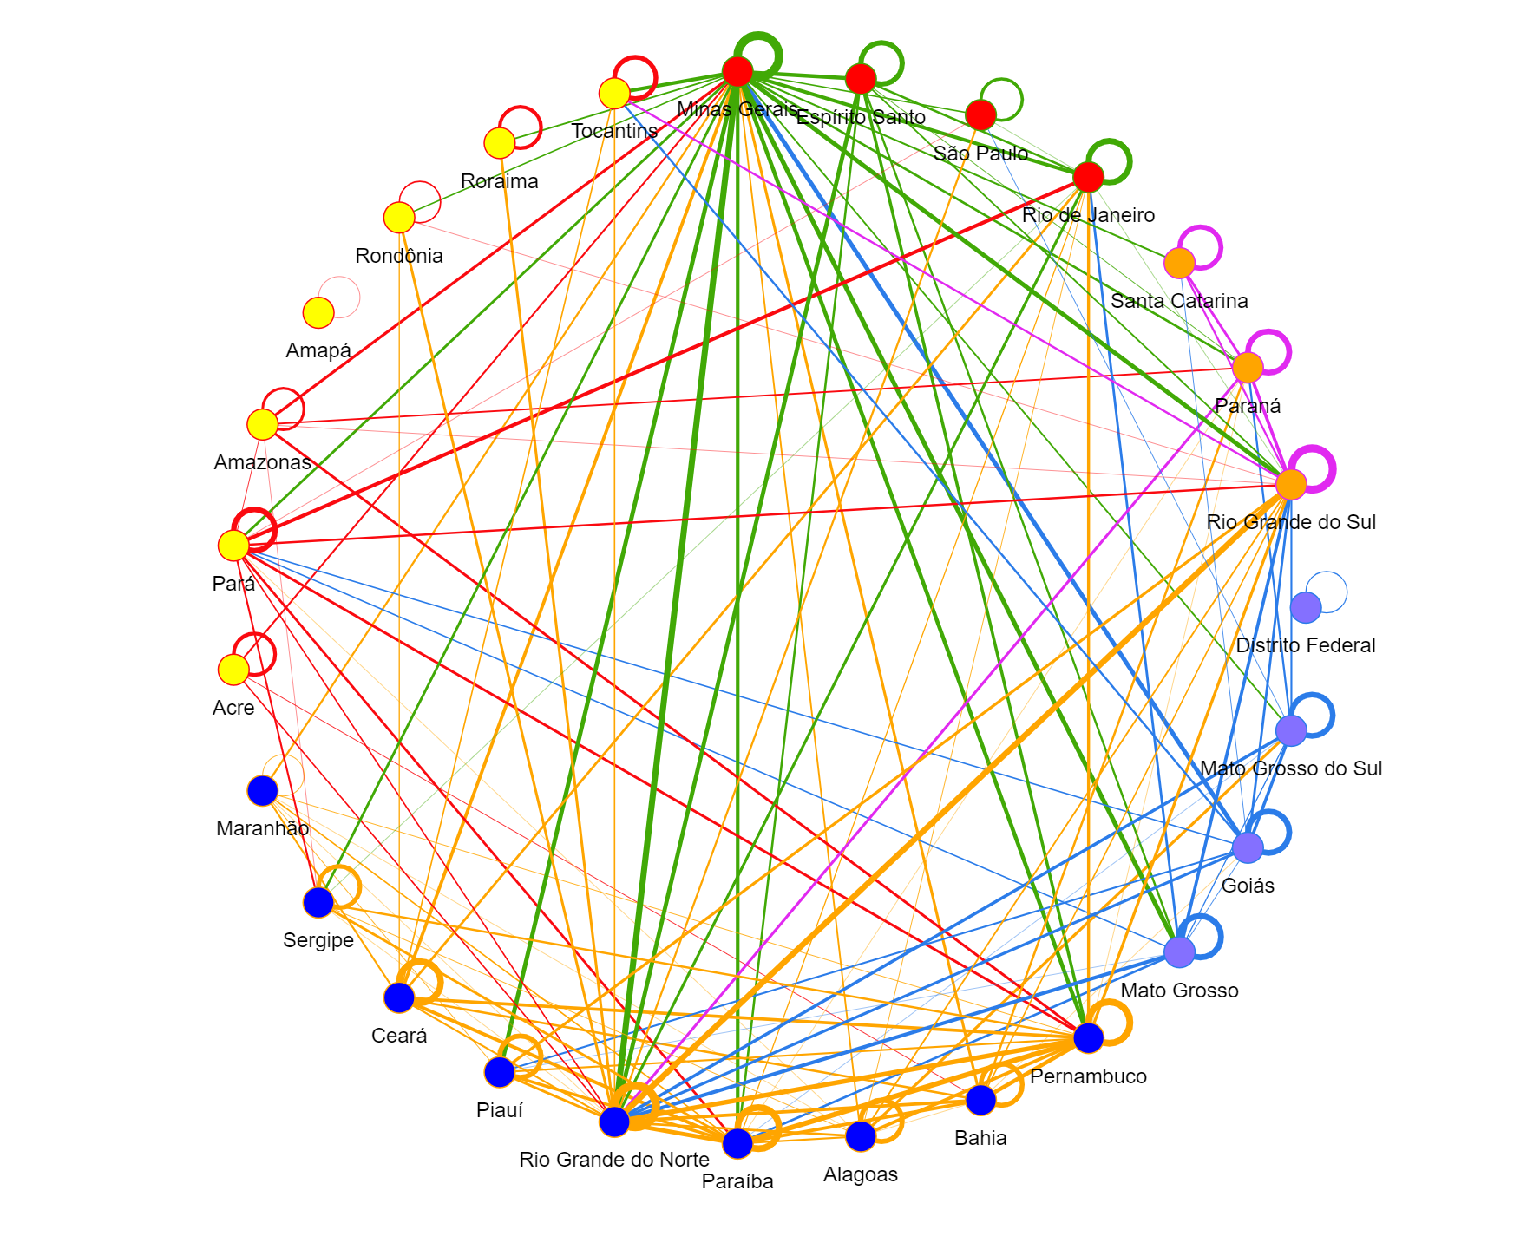
\includegraphics[width=0.35\textwidth]{Imagens/rede-agr-br-2011.pdf} &
		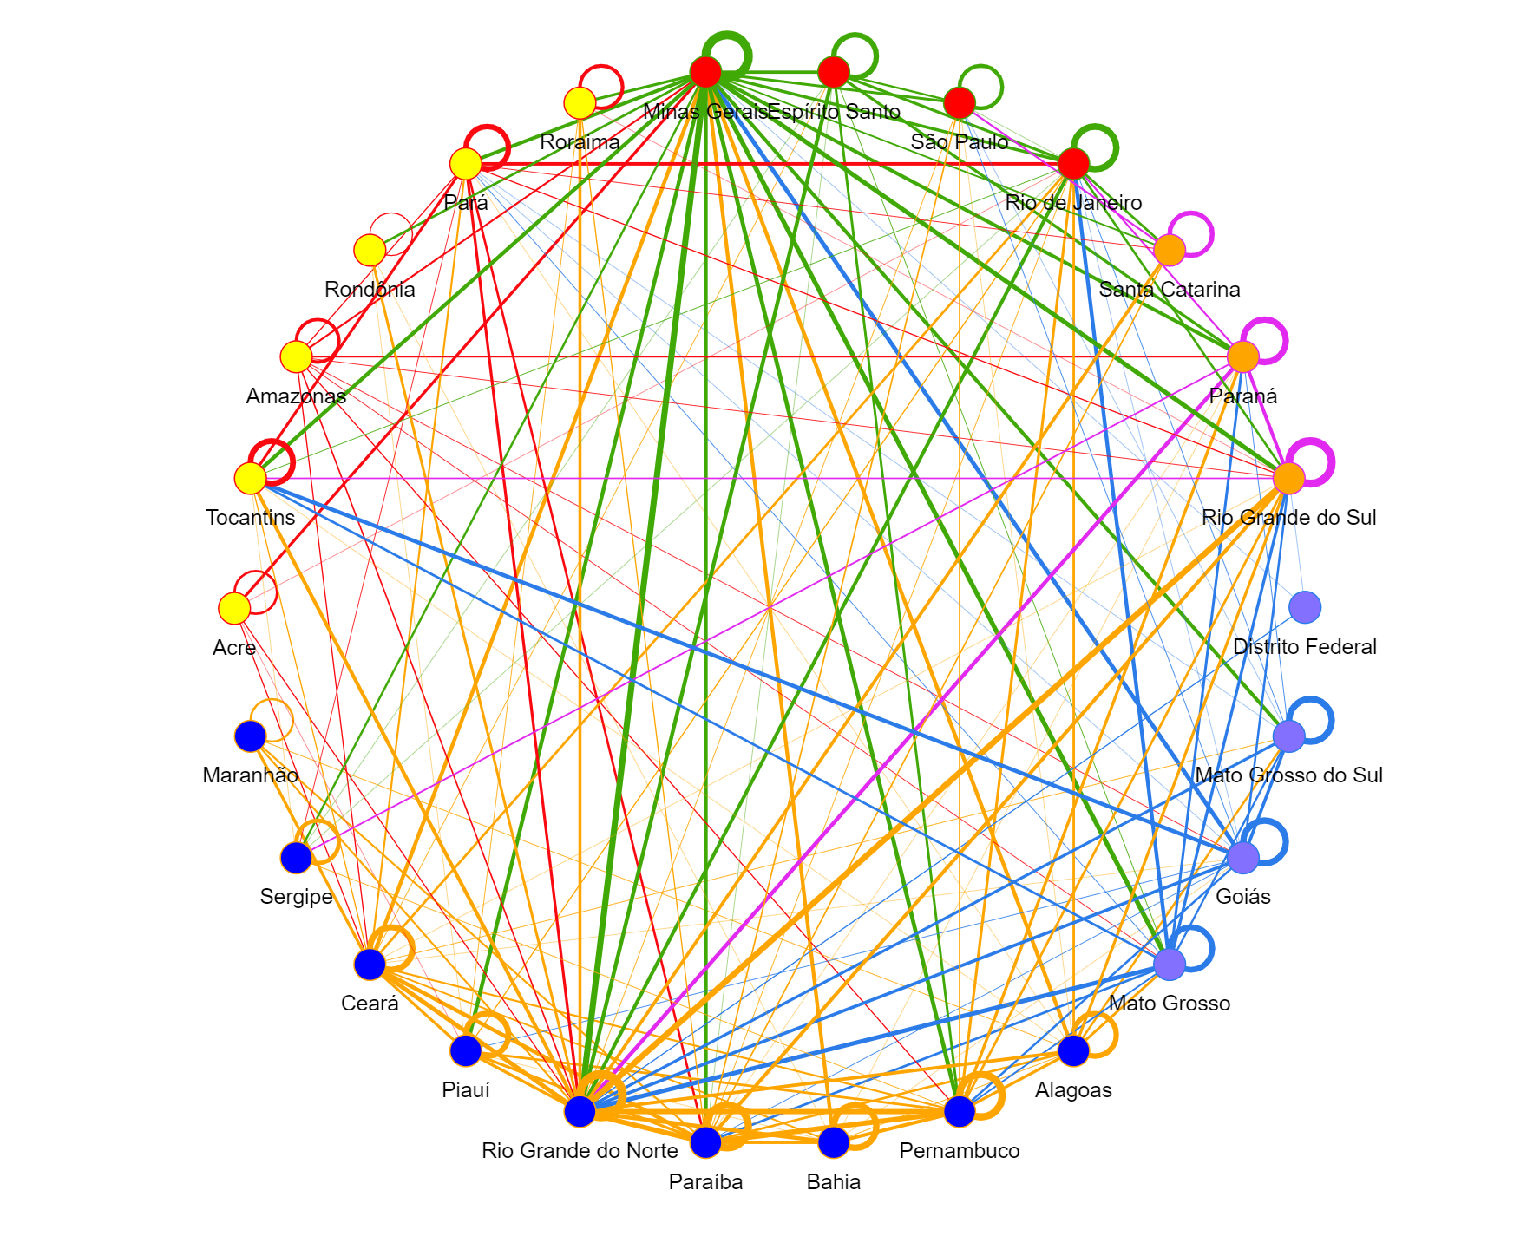
\includegraphics[width=0.35\textwidth]{Imagens/rede-agr-br-2012.pdf} &   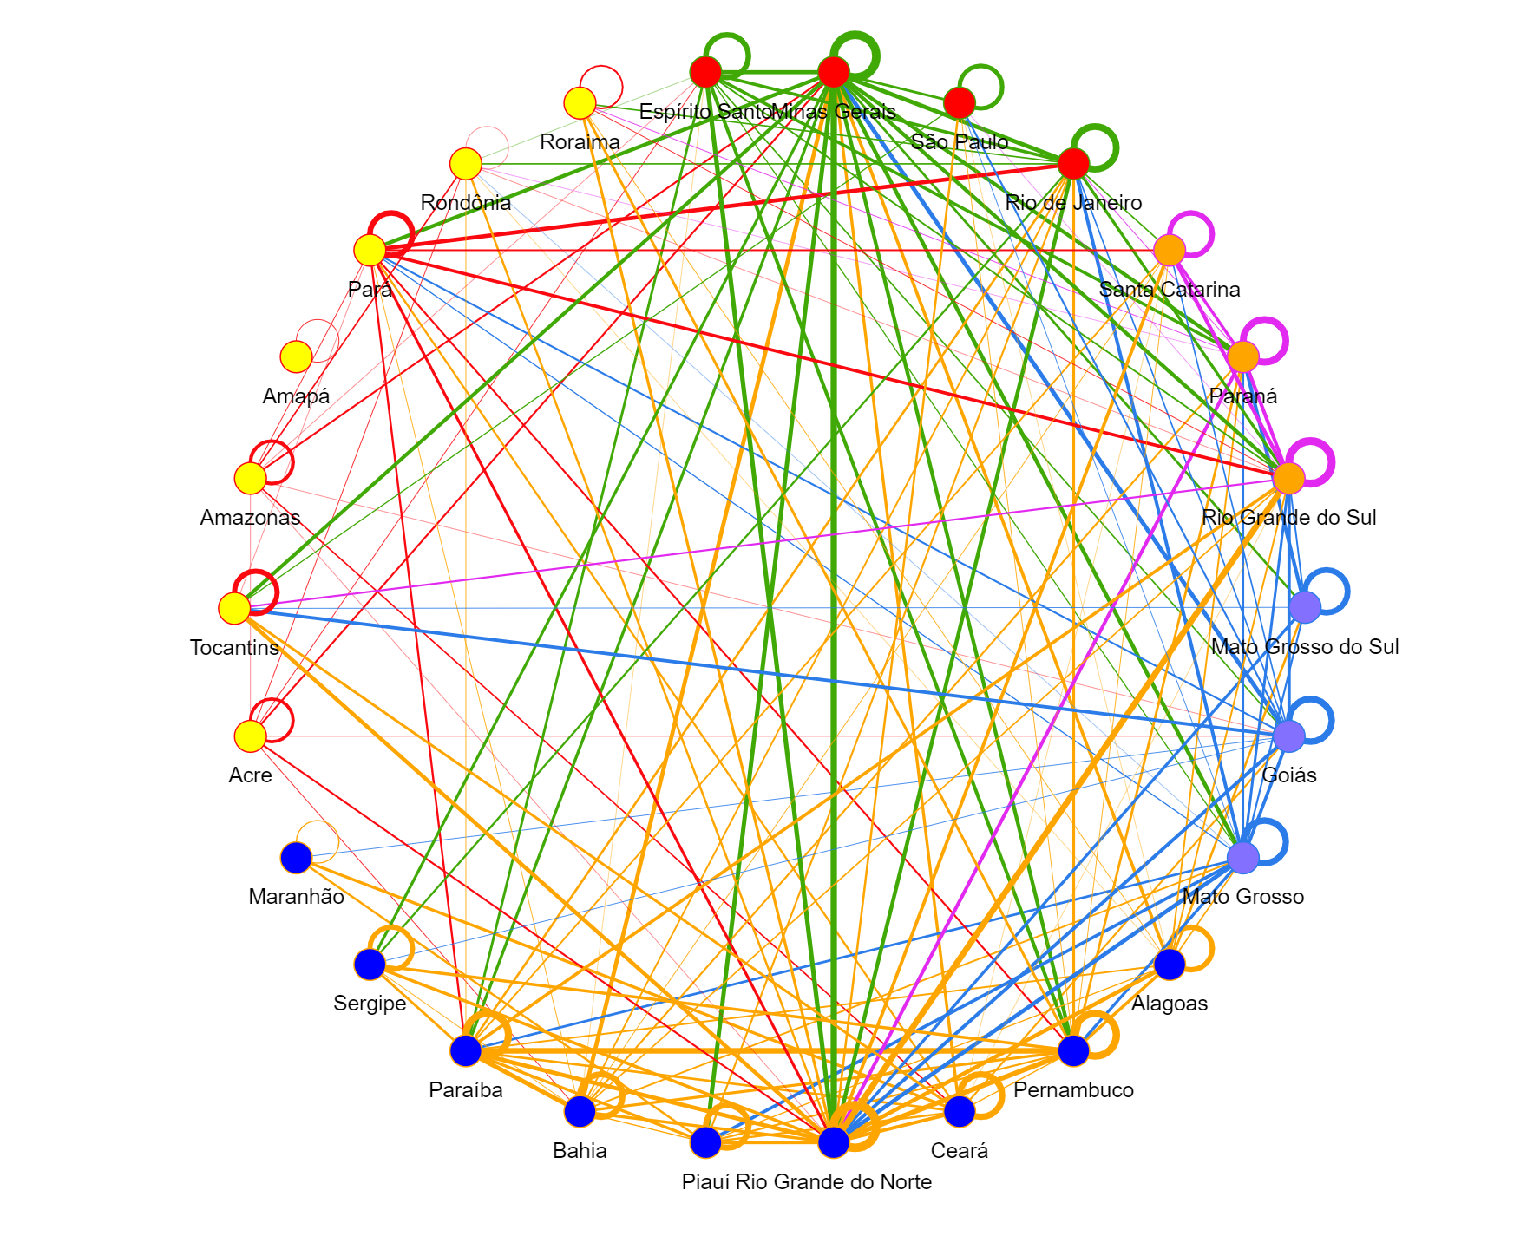
\includegraphics[width=0.35\textwidth]{Imagens/rede-agr-br-2013.pdf} \\
		2011 & 2012 & 2013\\[6pt]
		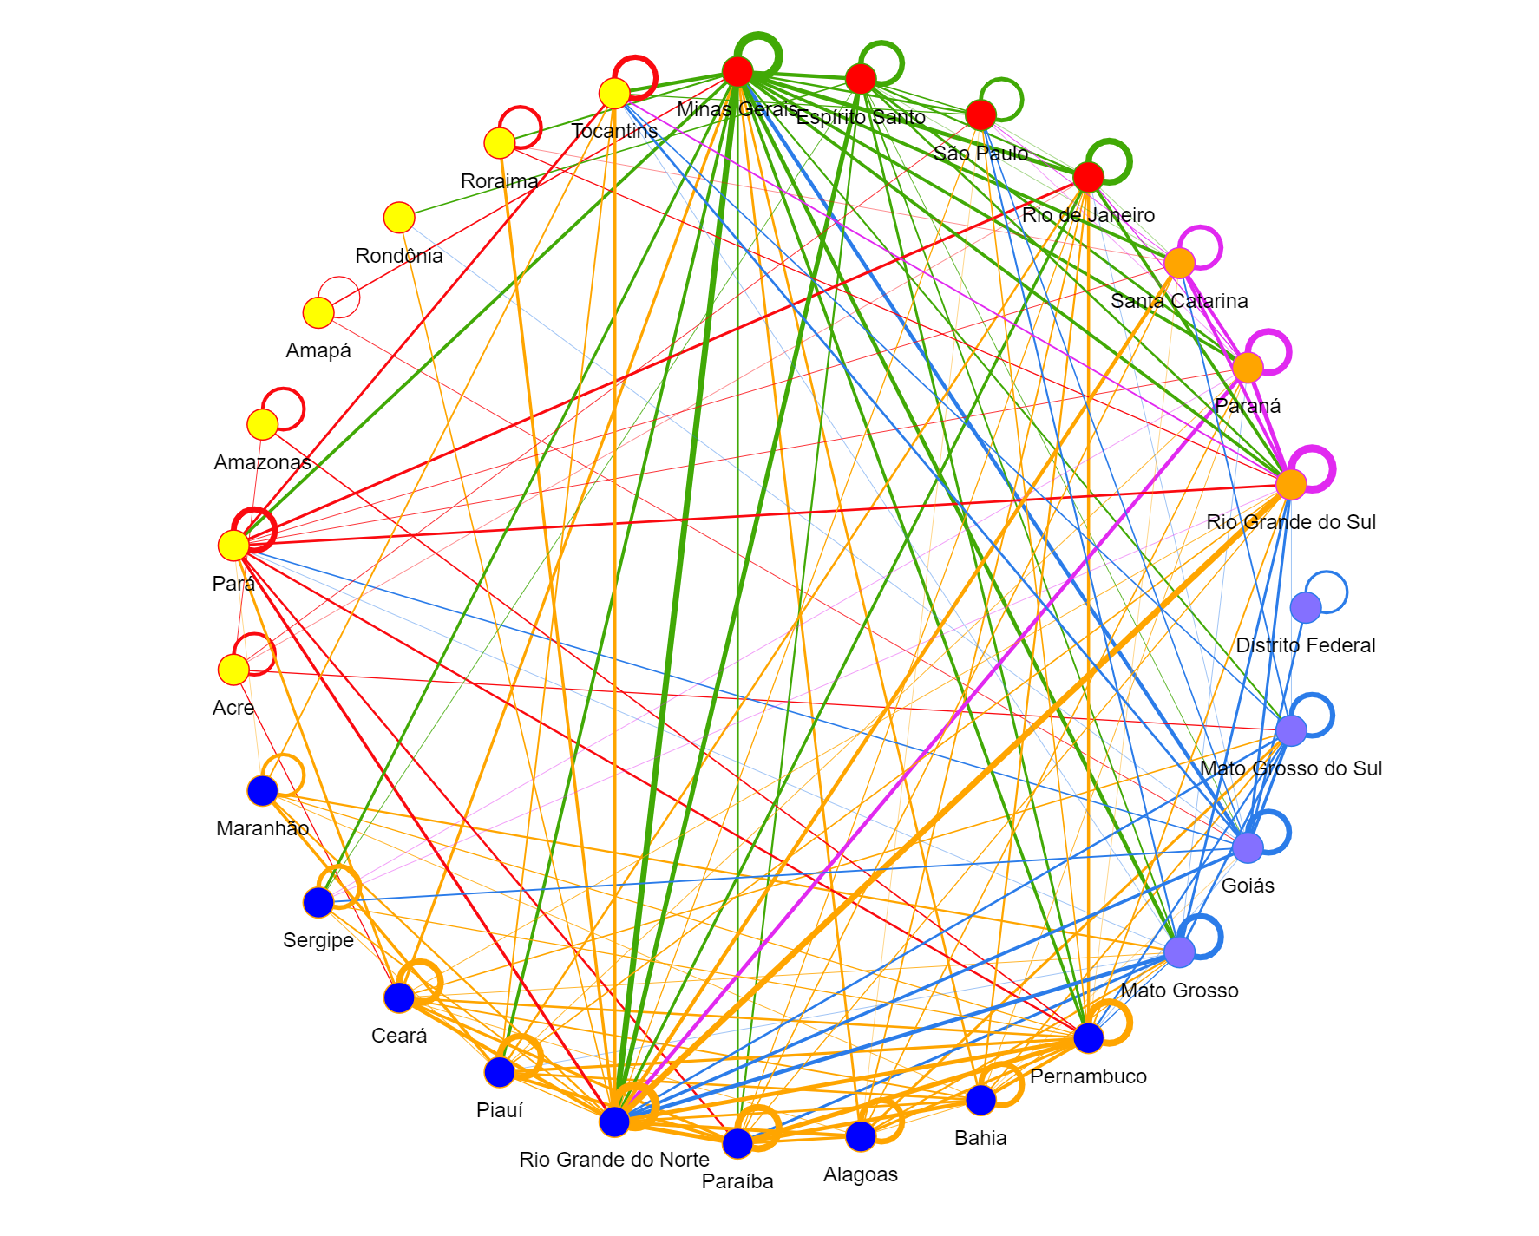
\includegraphics[width=0.35\textwidth]{Imagens/rede-agr-br-2014.pdf} &
		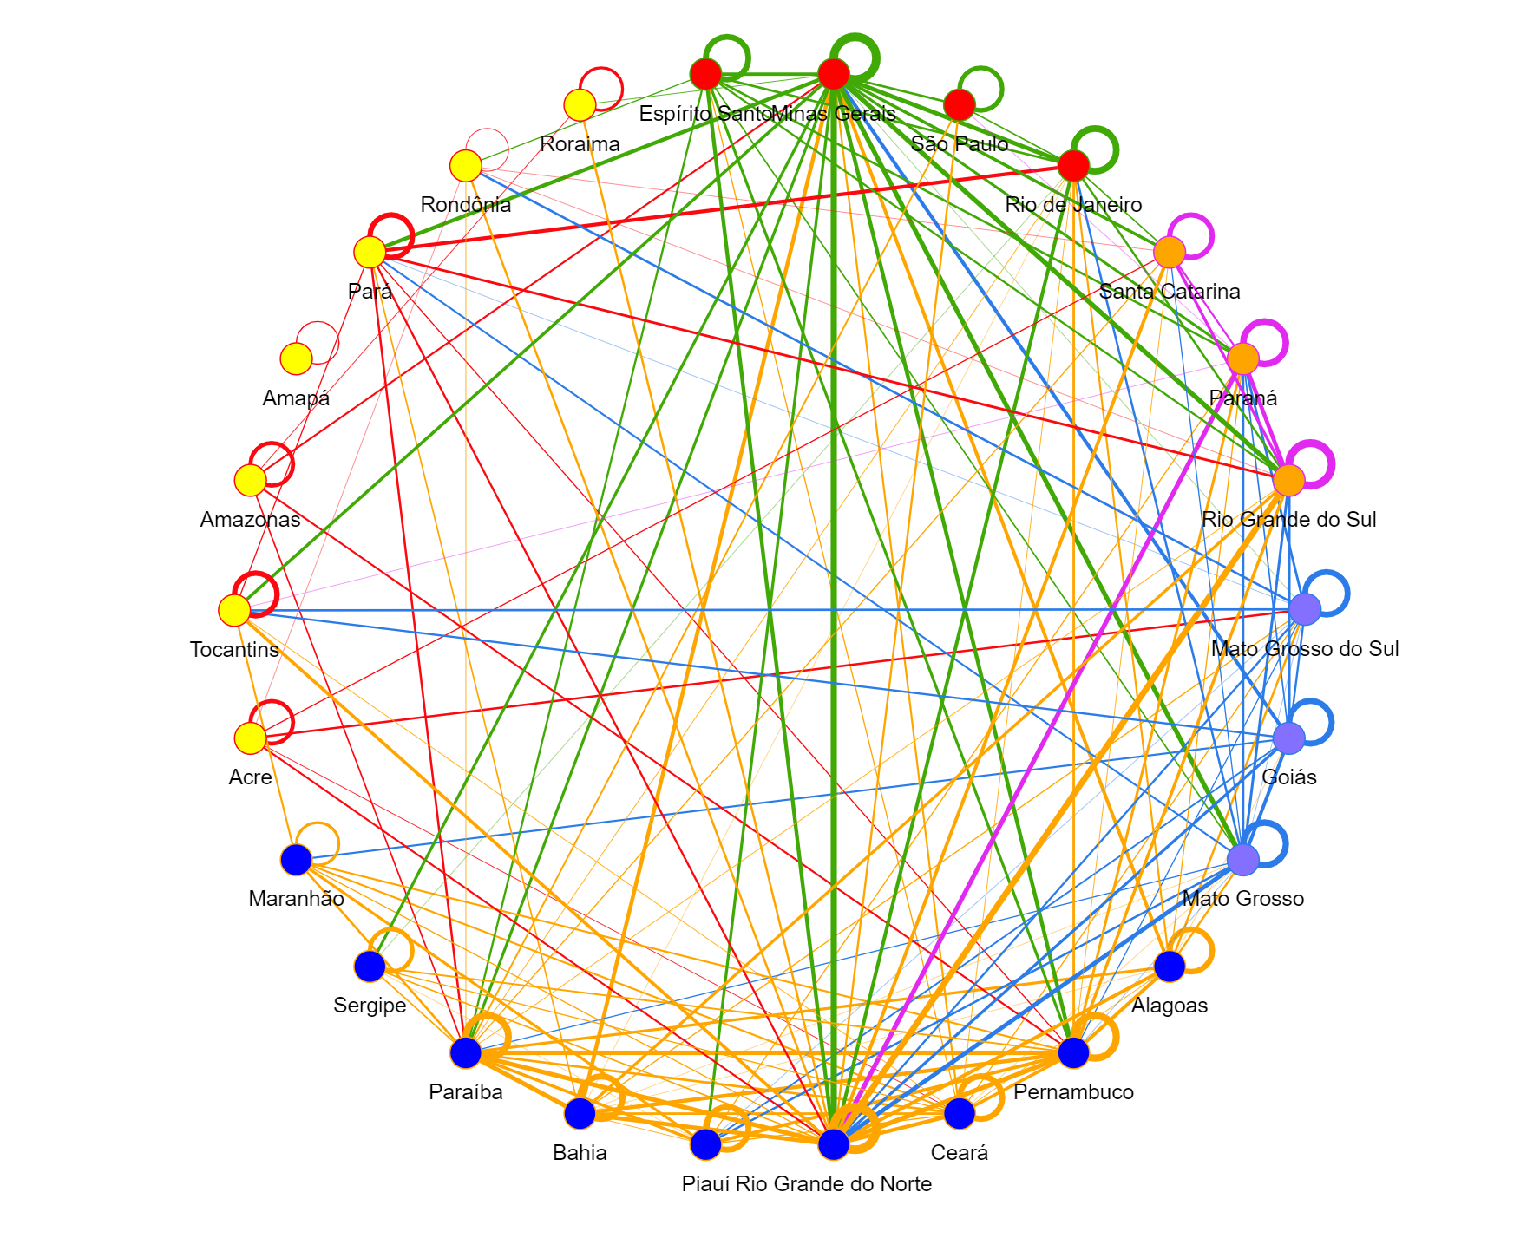
\includegraphics[width=0.35\textwidth]{Imagens/rede-agr-br-2015.pdf} &
		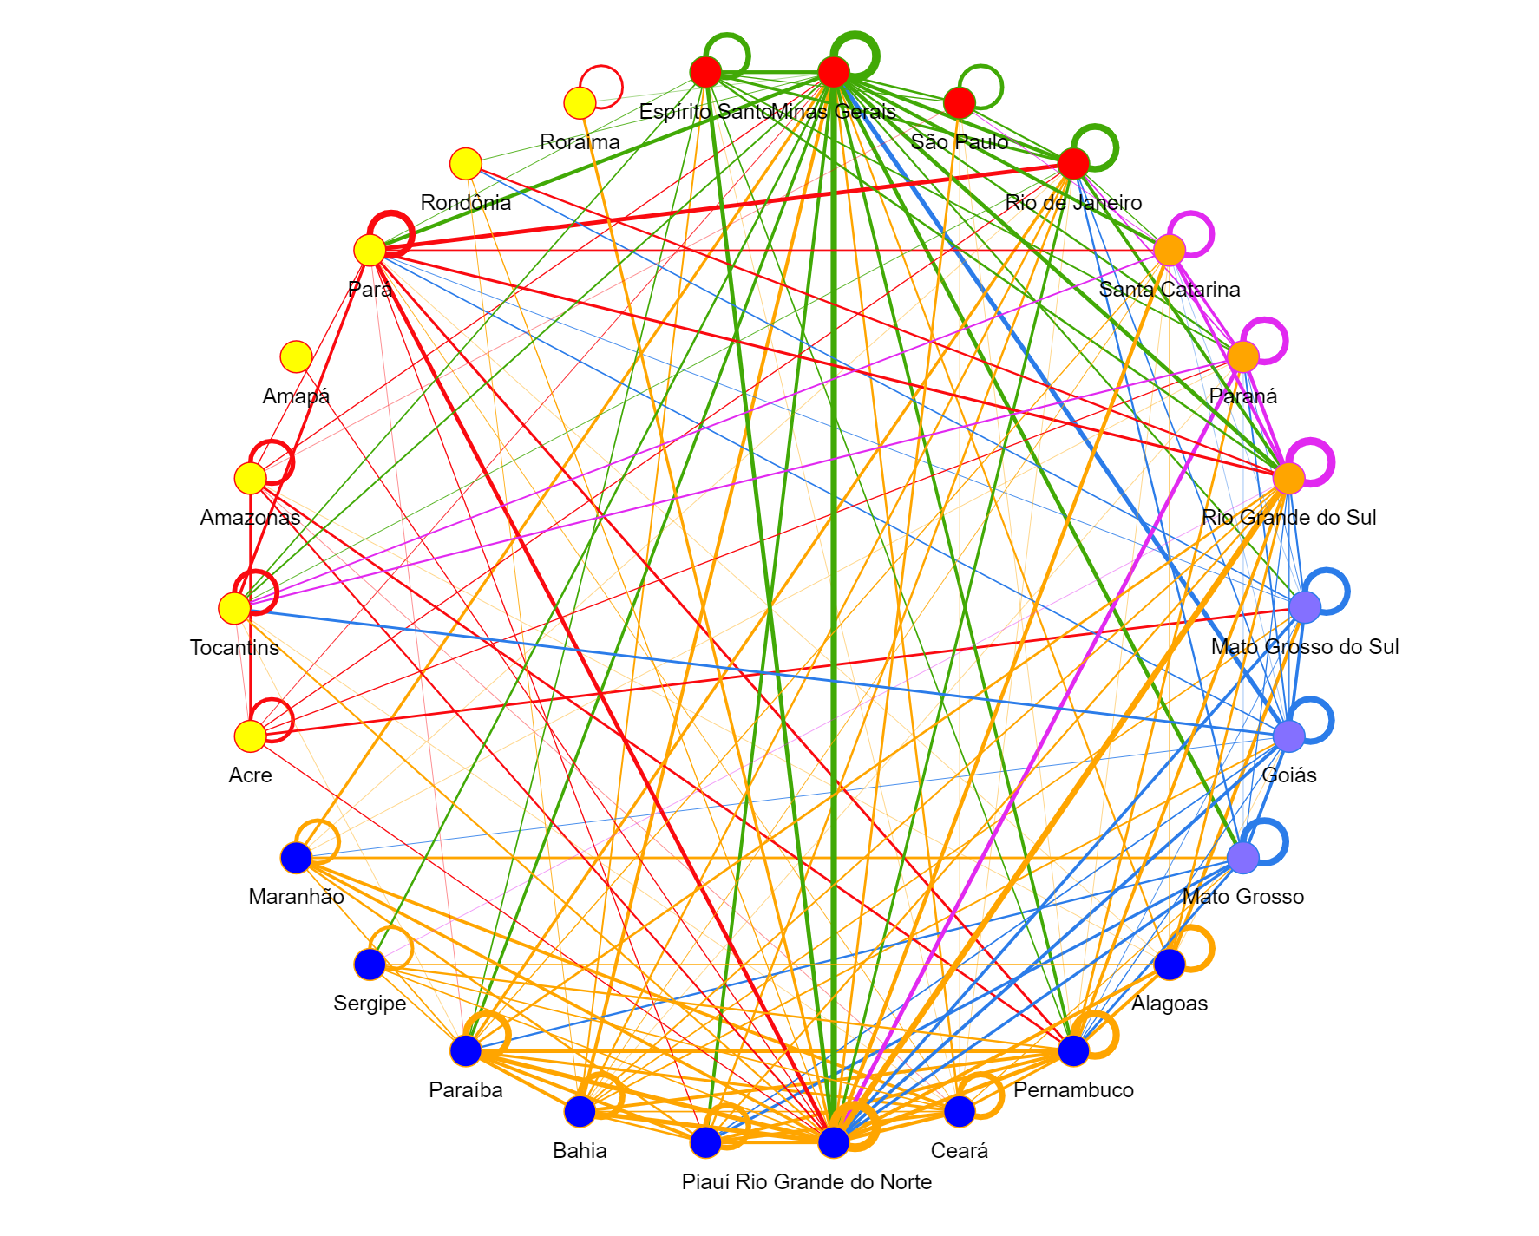
\includegraphics[width=0.35\textwidth]{Imagens/rede-agr-br-2016.pdf} \\
		2014 & 2015 & 2016\\[6pt]  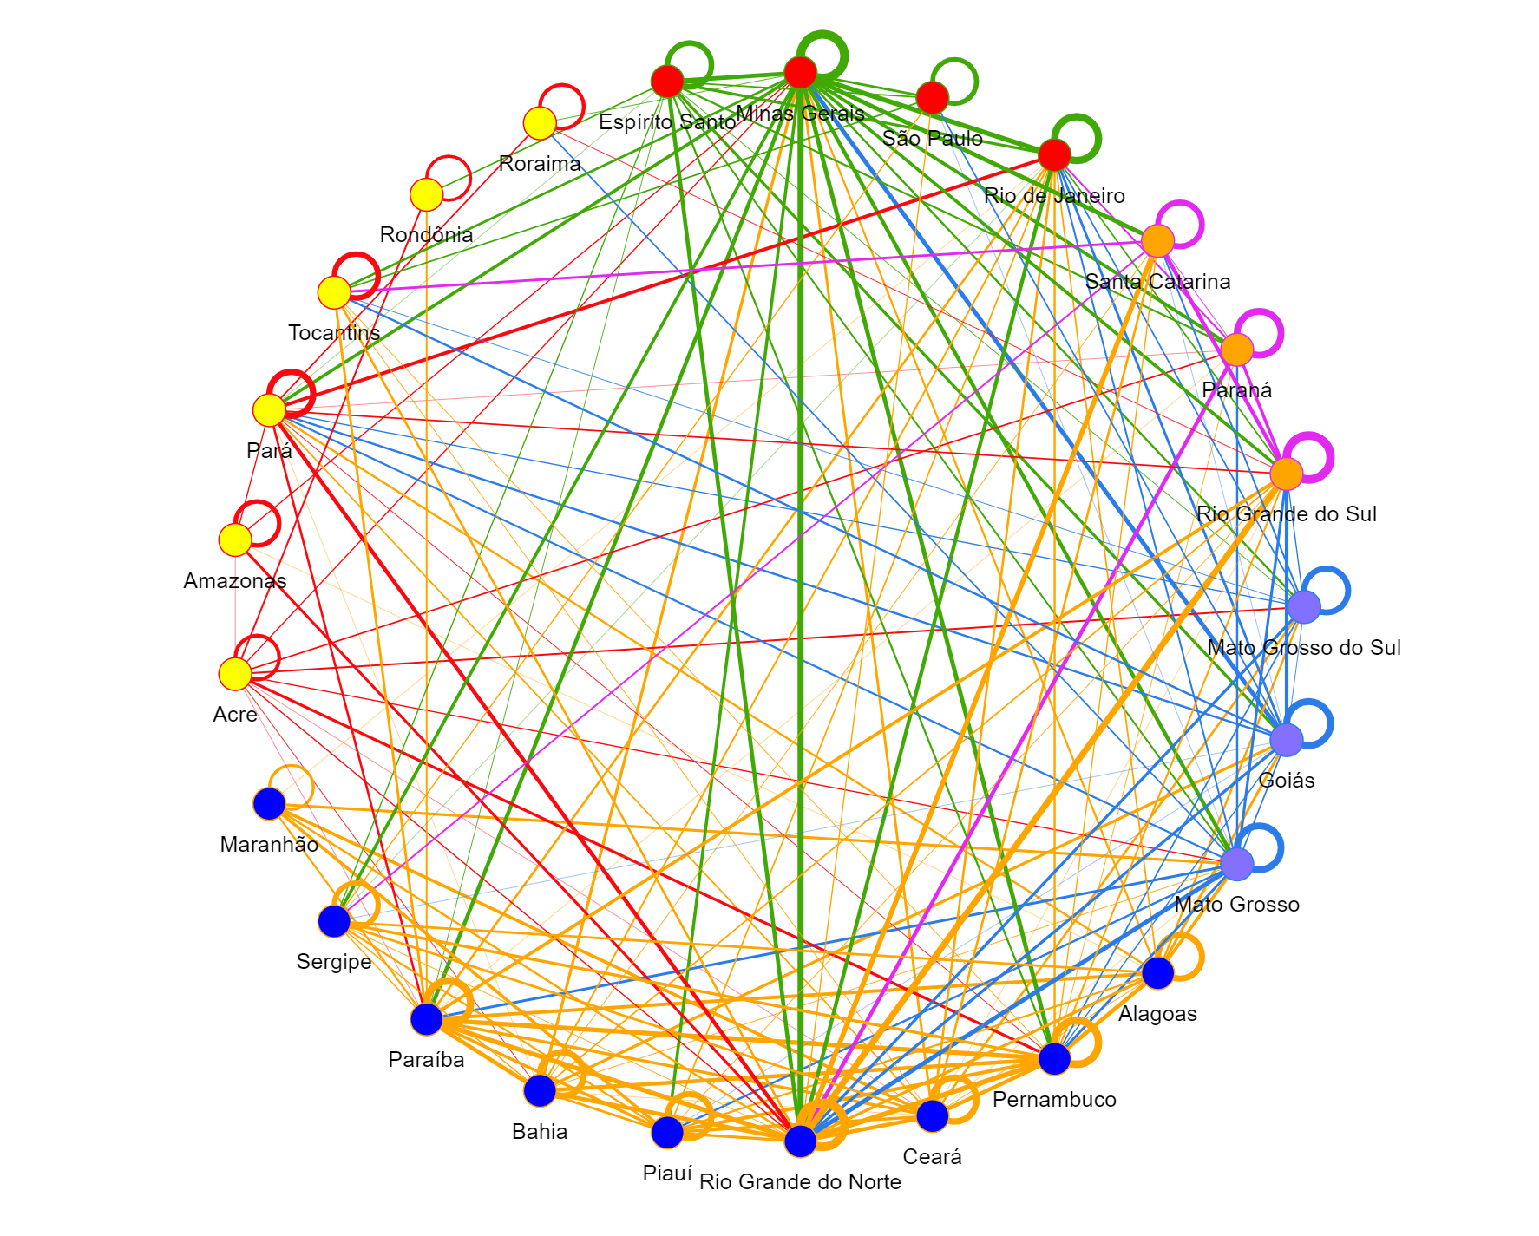
\includegraphics[width=0.35\textwidth]{Imagens/rede-agr-br-2017.pdf} & & \\
		2017 & & \\
	\end{tabular}
	\caption{Redes de Coautoria Universidades Federal do Brasil: Área: \textit{Agricultural Sciences}}
\end{figure}

\subsubsection{Rede de Coautoria Brasil - Vértice Focal Alagoas}

\begin{figure}[H]
	\begin{tabular}{ccc}
		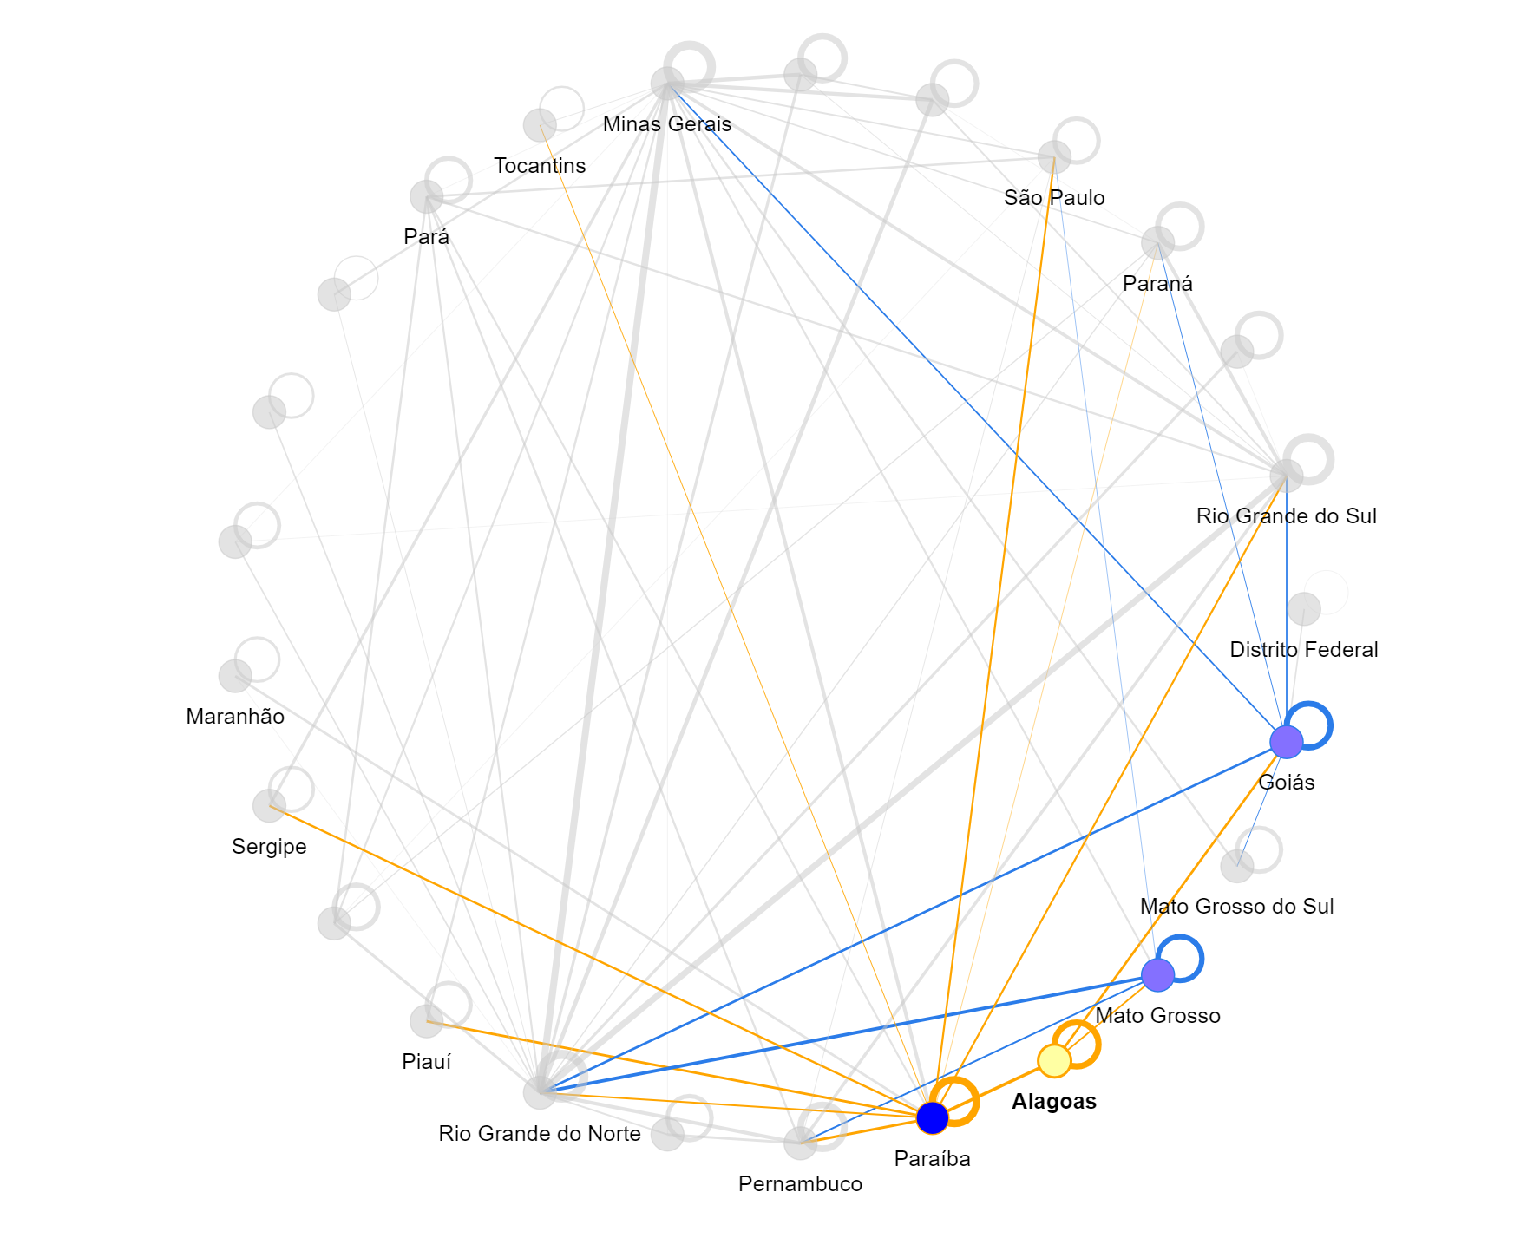
\includegraphics[width=0.38\textwidth]{Imagens/rede-agr-AL-2008.pdf} &   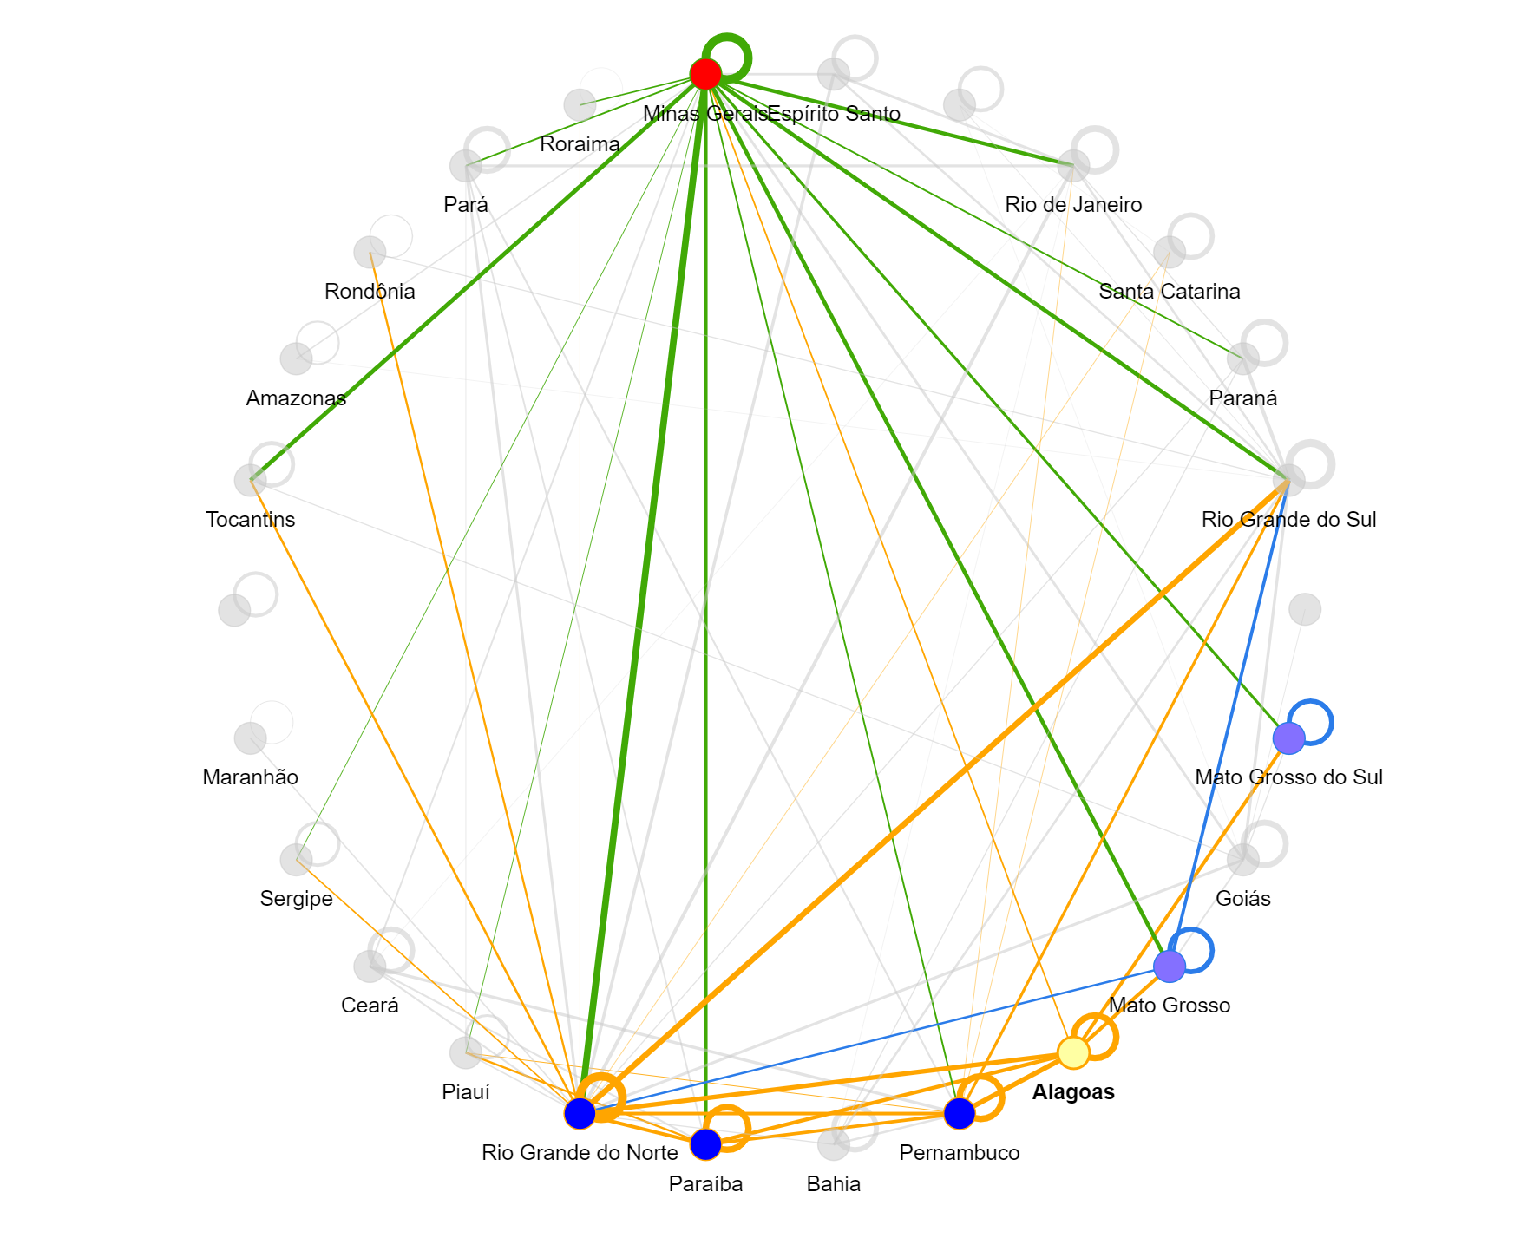
\includegraphics[width=0.38\textwidth]{Imagens/rede-agr-AL-2009.pdf} &
		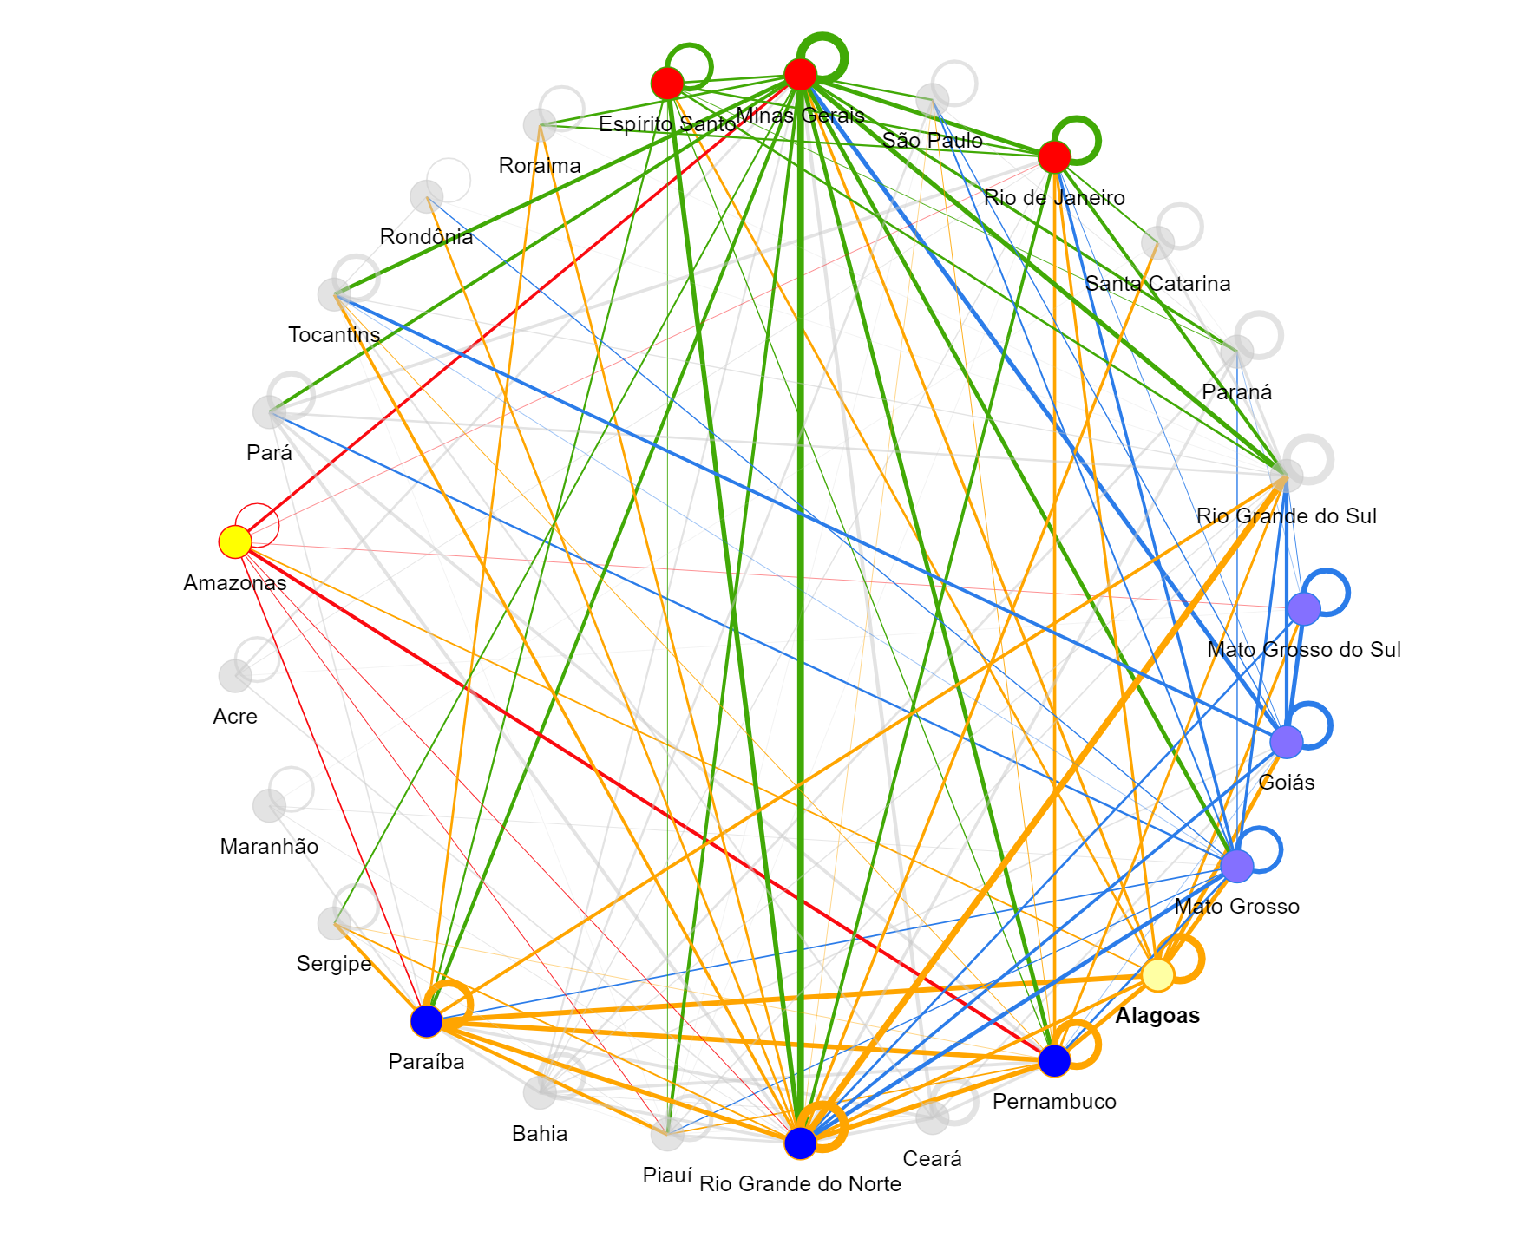
\includegraphics[width=0.38\textwidth]{Imagens/rede-agr-AL-2010.pdf}\\
		2008 & 2009 & 2010\\[6pt] 
		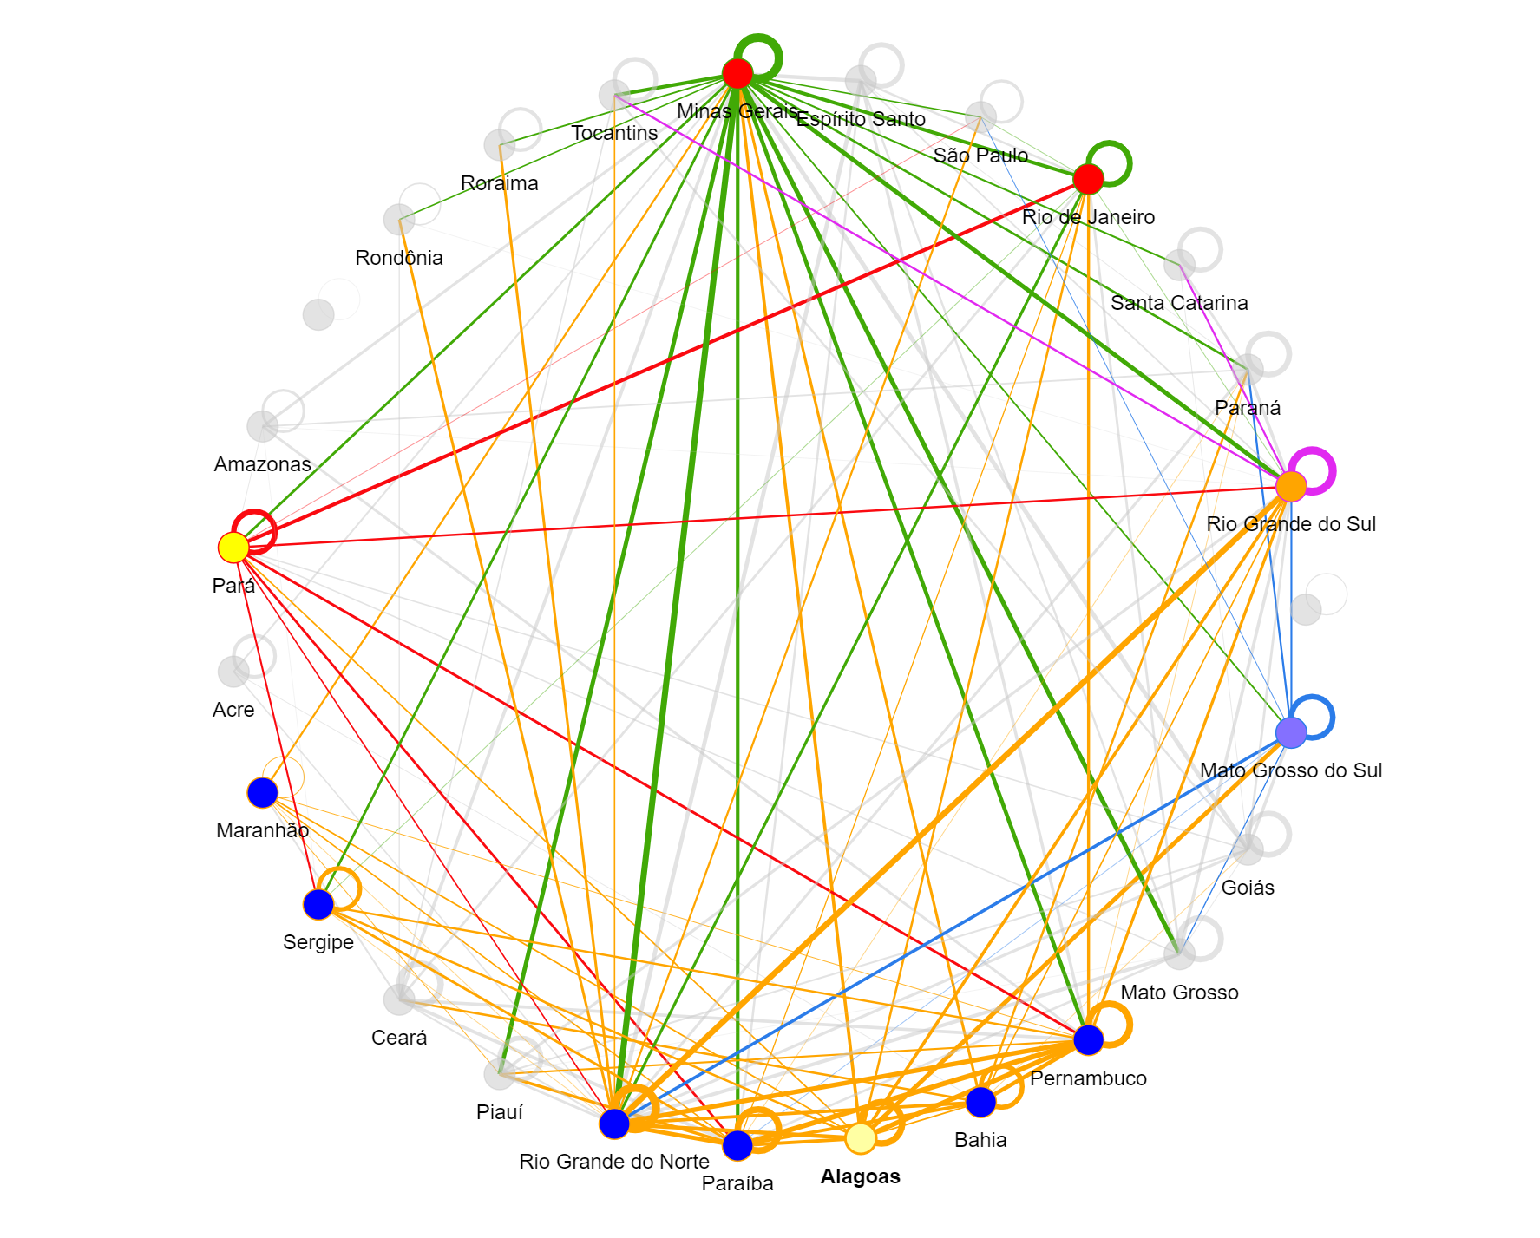
\includegraphics[width=0.38\textwidth]{Imagens/rede-agr-AL-2011.pdf} &
		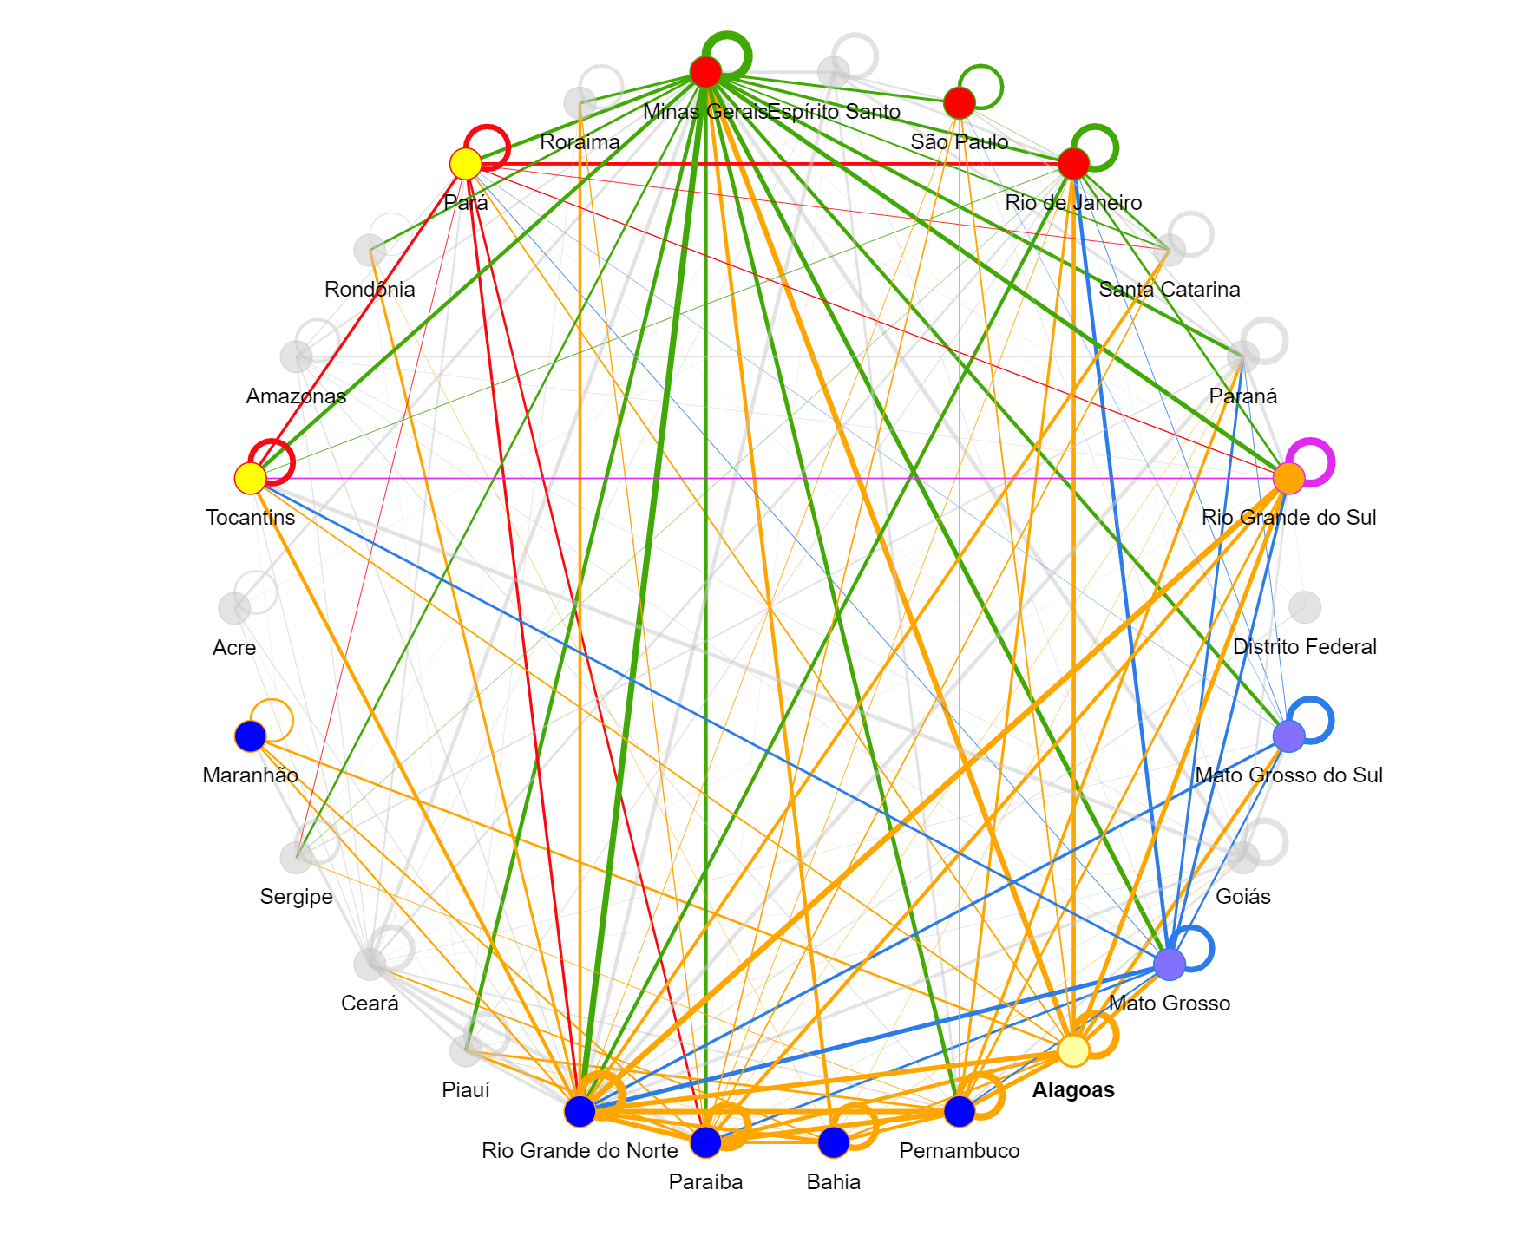
\includegraphics[width=0.38\textwidth]{Imagens/rede-agr-AL-2012.pdf} &   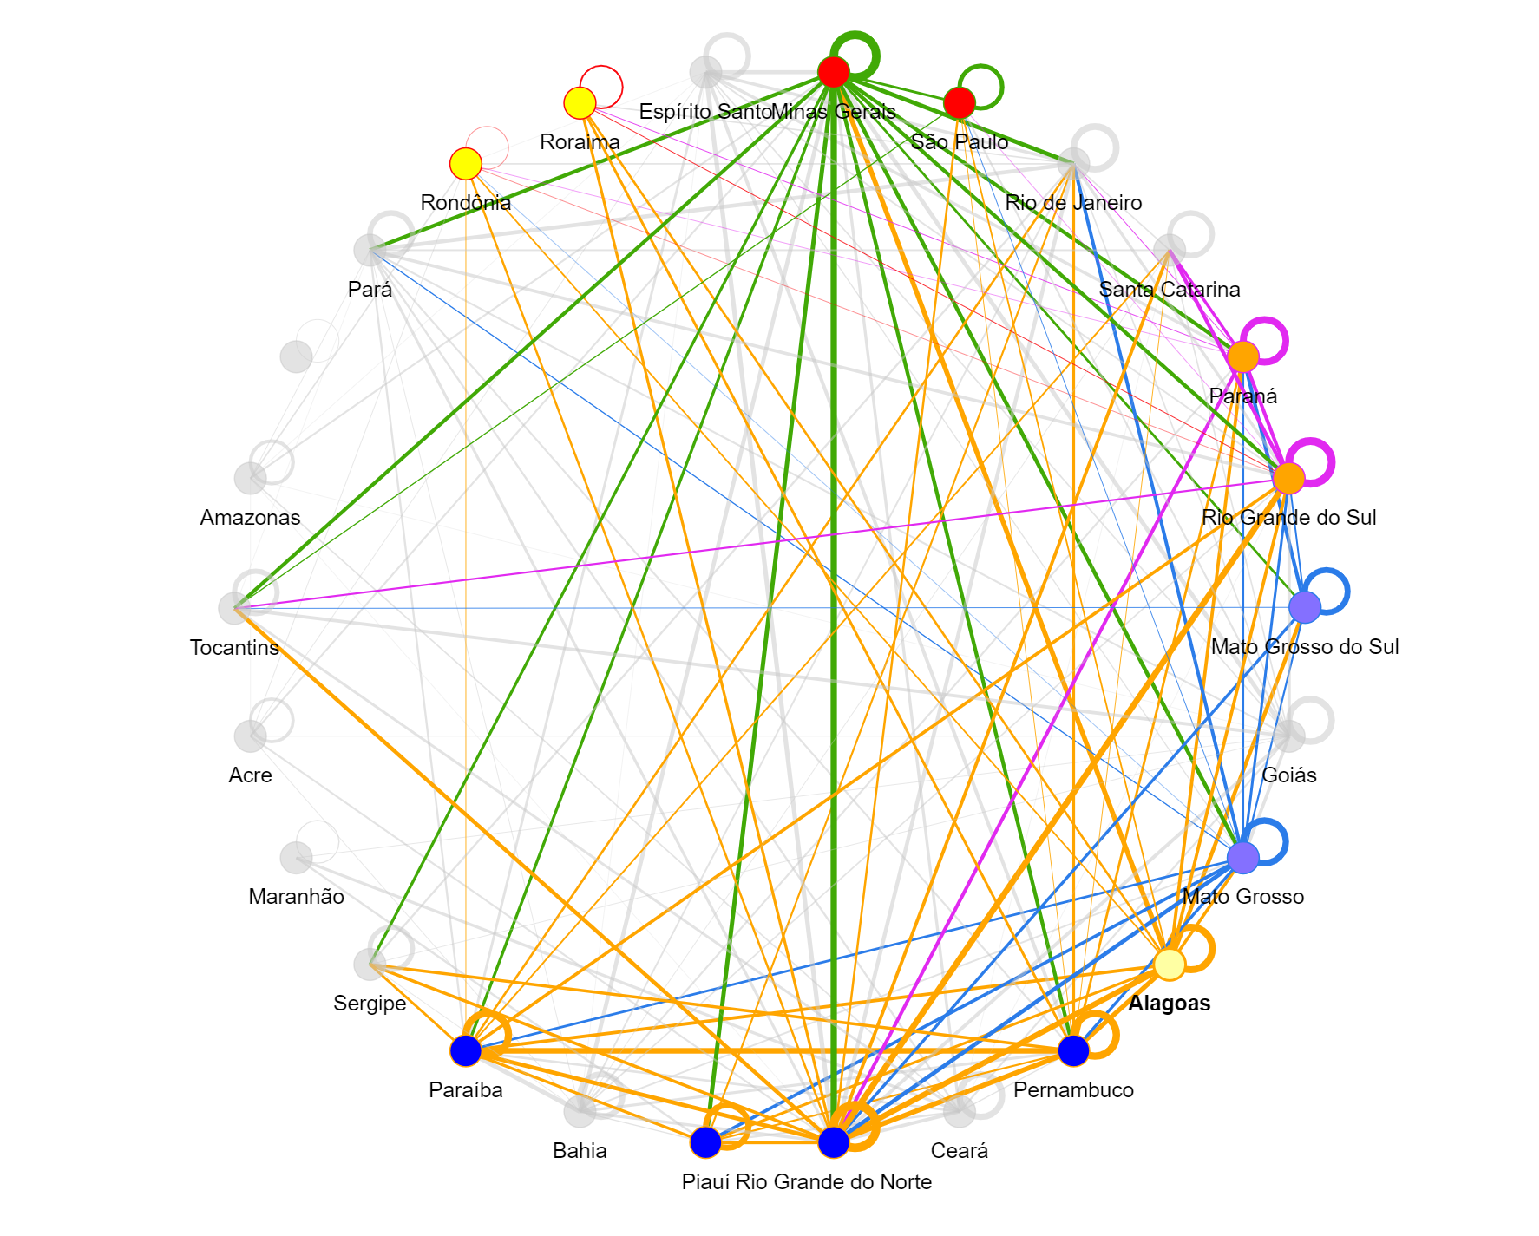
\includegraphics[width=0.38\textwidth]{Imagens/rede-agr-AL-2013.pdf} \\
		2011 & 2012 & 2013\\[6pt]
		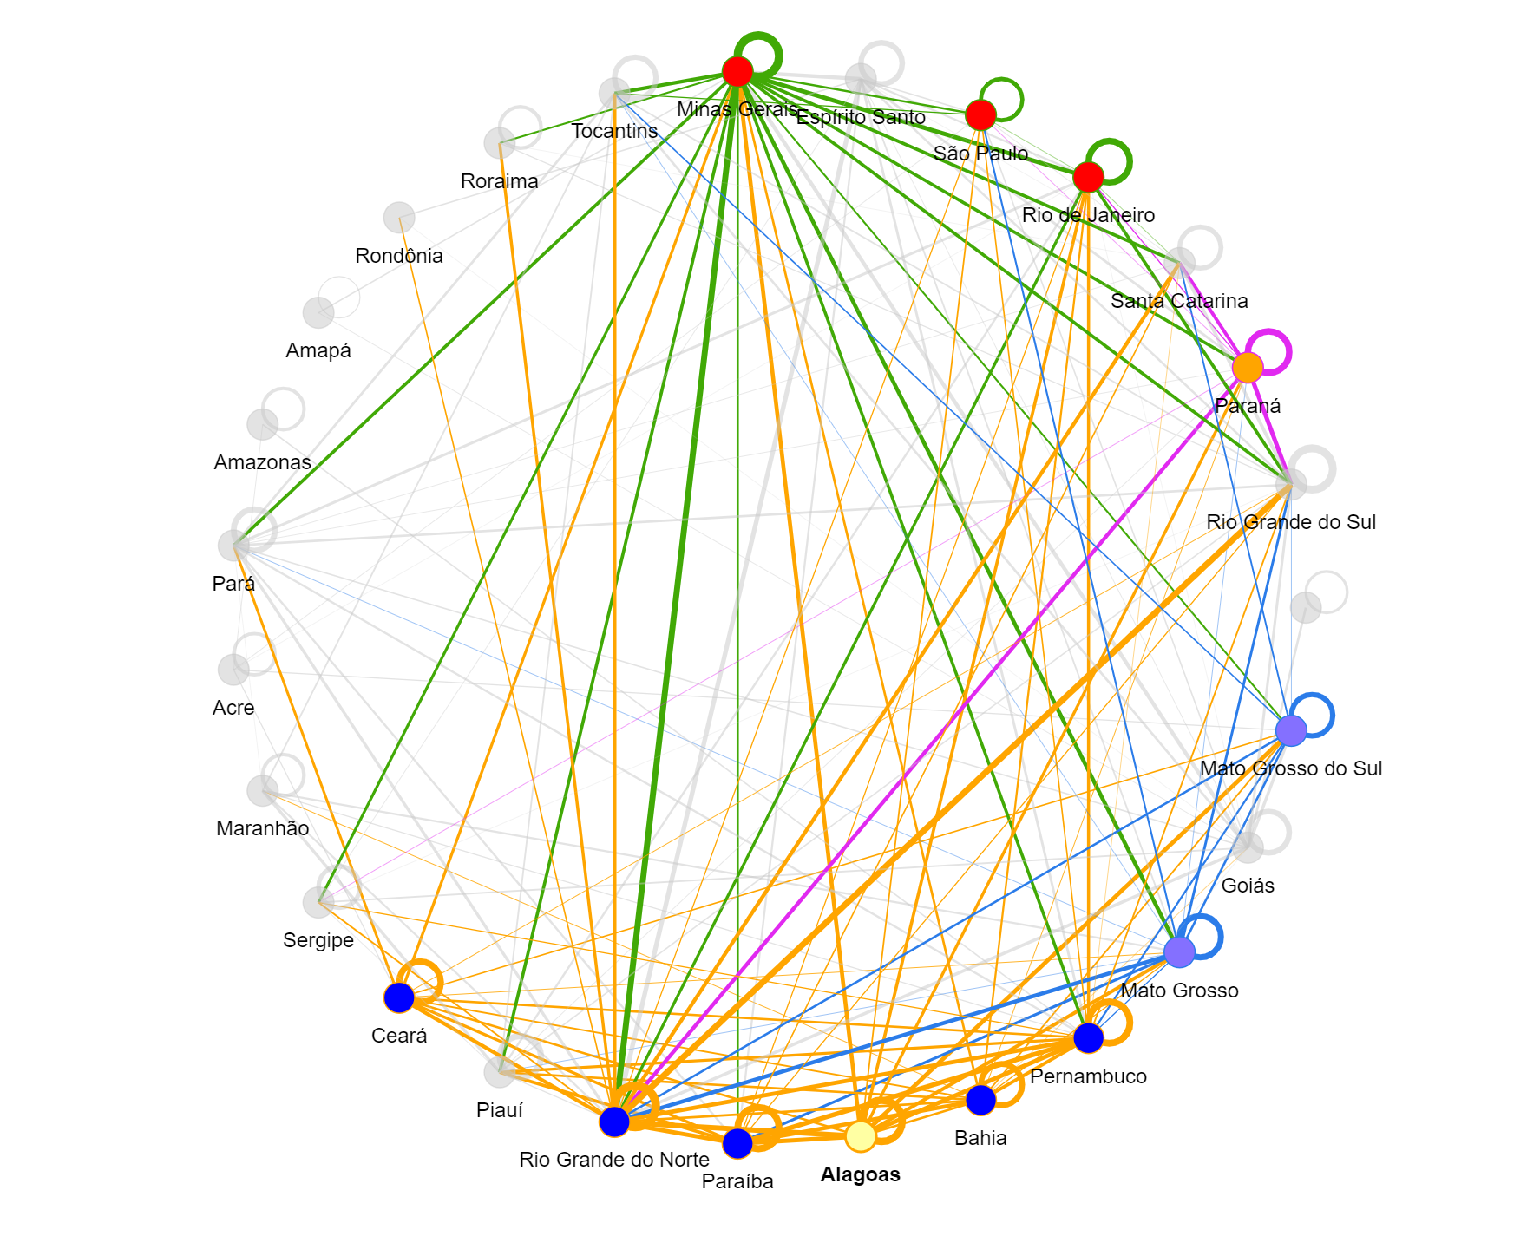
\includegraphics[width=0.38\textwidth]{Imagens/rede-agr-AL-2014.pdf} &
		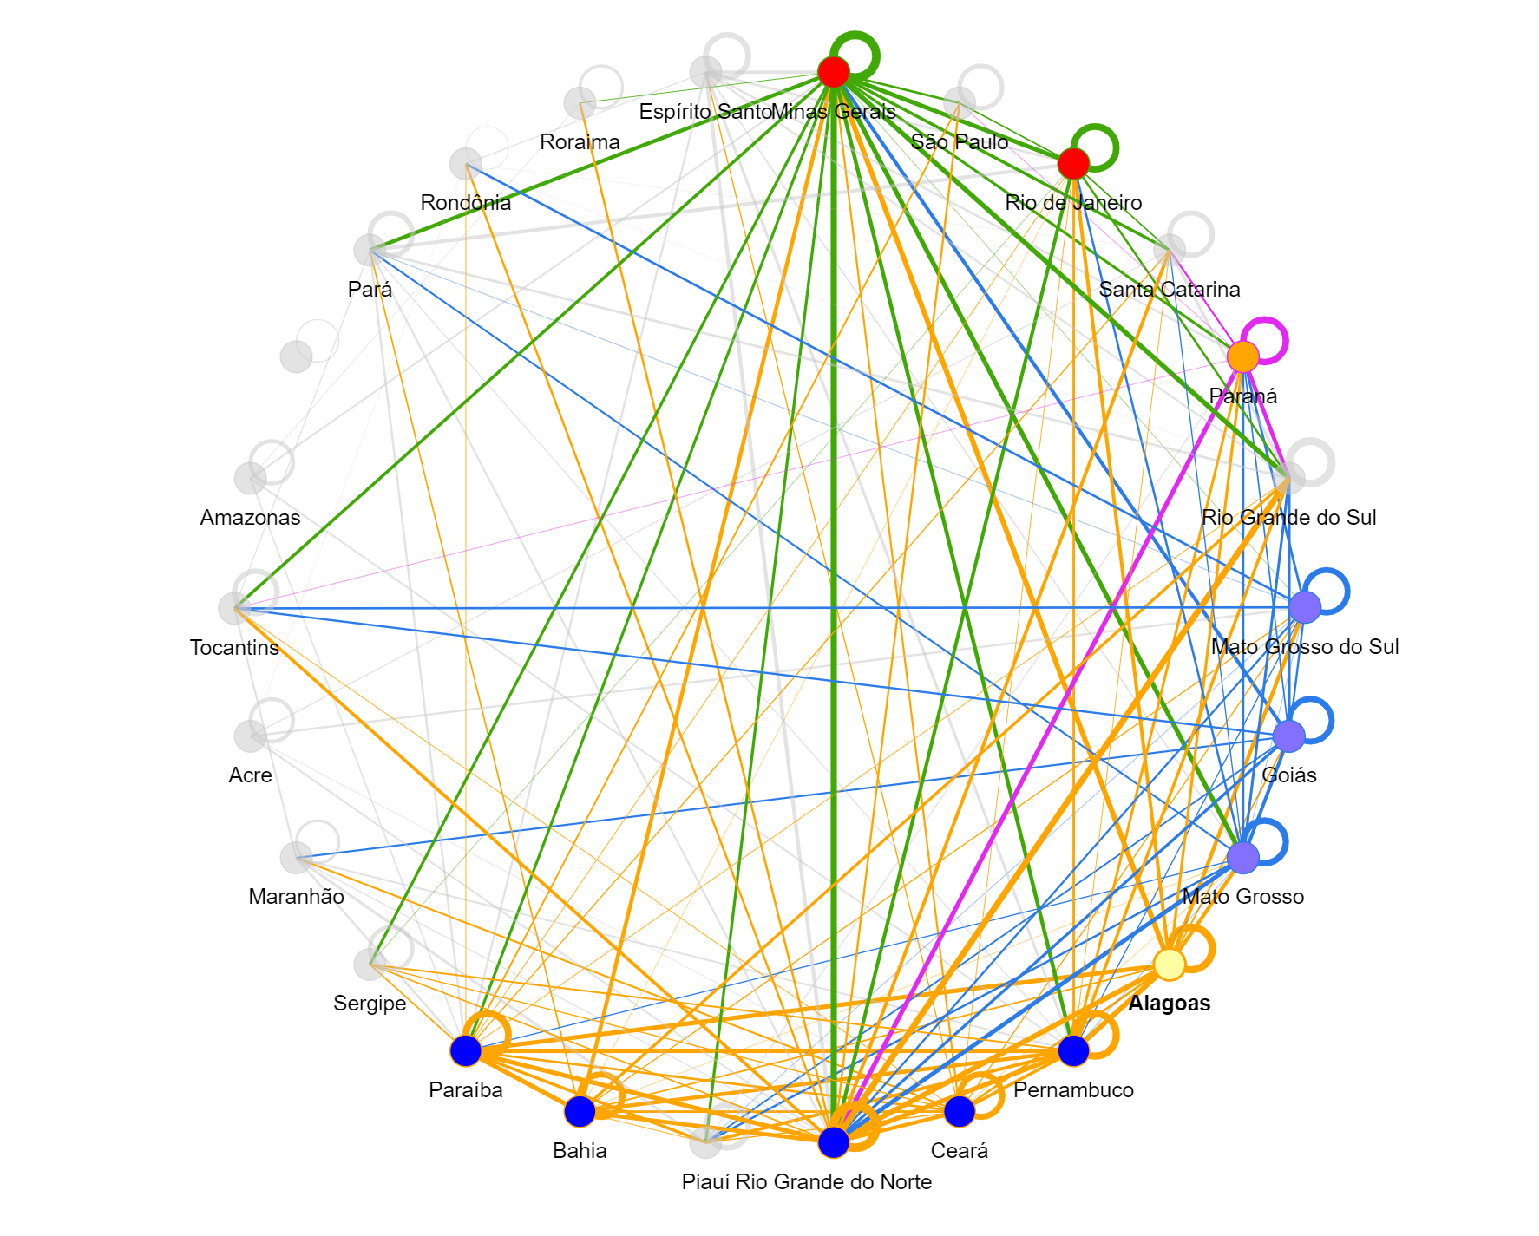
\includegraphics[width=0.38\textwidth]{Imagens/rede-agr-AL-2015.pdf} &
		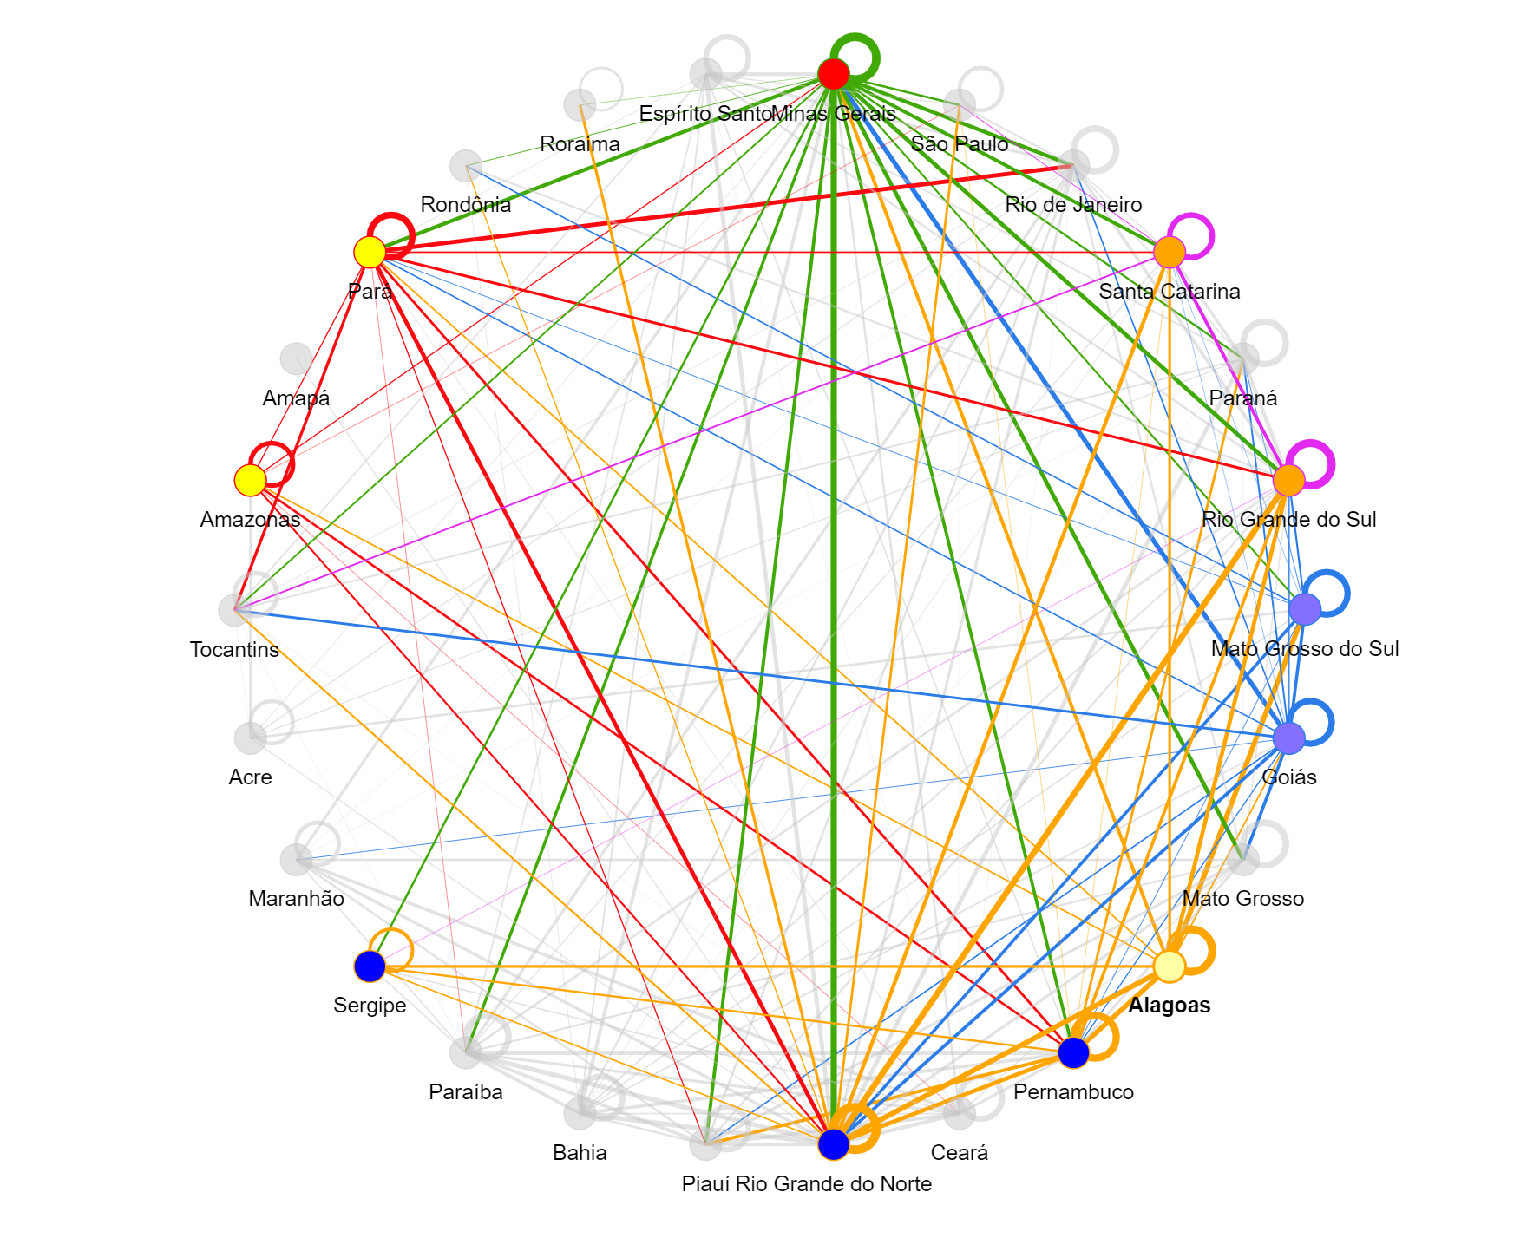
\includegraphics[width=0.38\textwidth]{Imagens/rede-agr-AL-2016.pdf} \\
		2014 & 2015 & 2016\\[6pt]  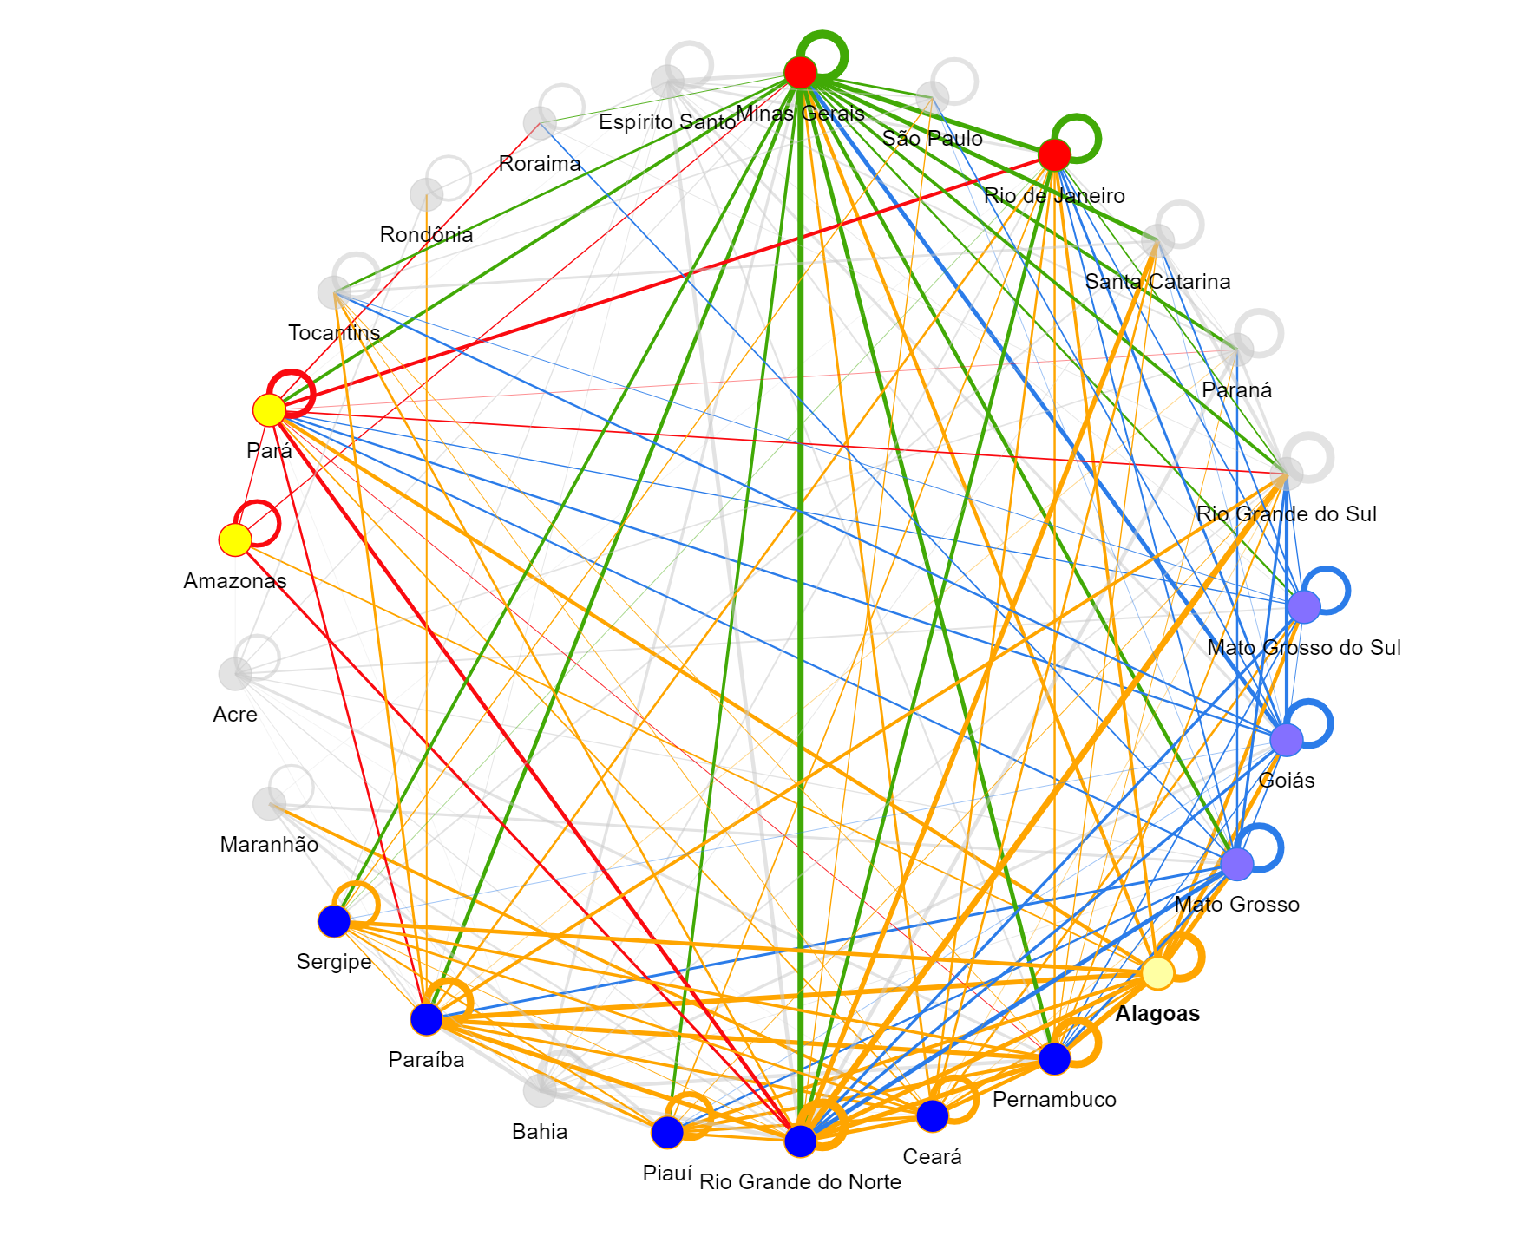
\includegraphics[width=0.38\textwidth]{Imagens/rede-agr-AL-2017.pdf} & & \\
		2017 & & \\
	\end{tabular}
	\caption{Redes de Coautoria da Universidade Federal de Alagoas - Área \textit{Agricultural Sciences}}
\end{figure}


\section{\textbf{Exact and Earth Sciences}}

\subsubsection{Rede de Coautoria das Universidade Federais do Brasil}

\begin{figure}[H]
	\begin{tabular}{ccc}
		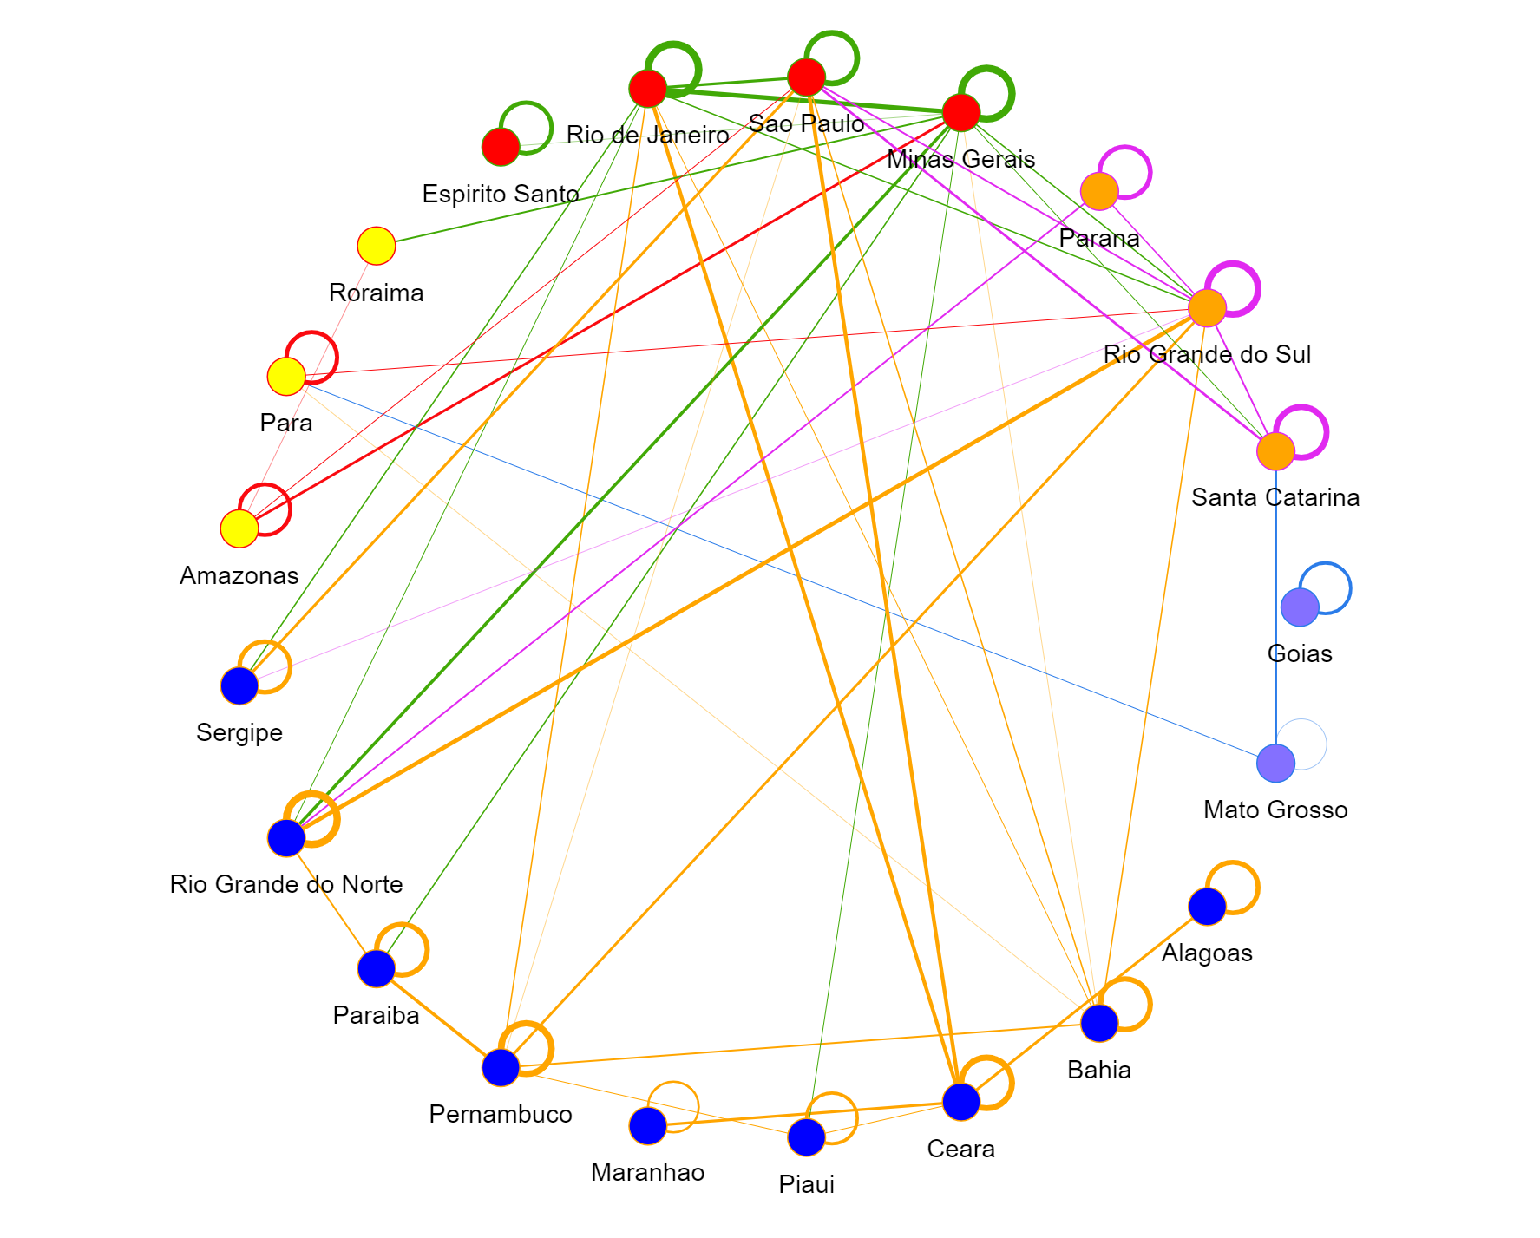
\includegraphics[width=0.35\textwidth]{Imagens/rede-exact-br-2008.pdf} &   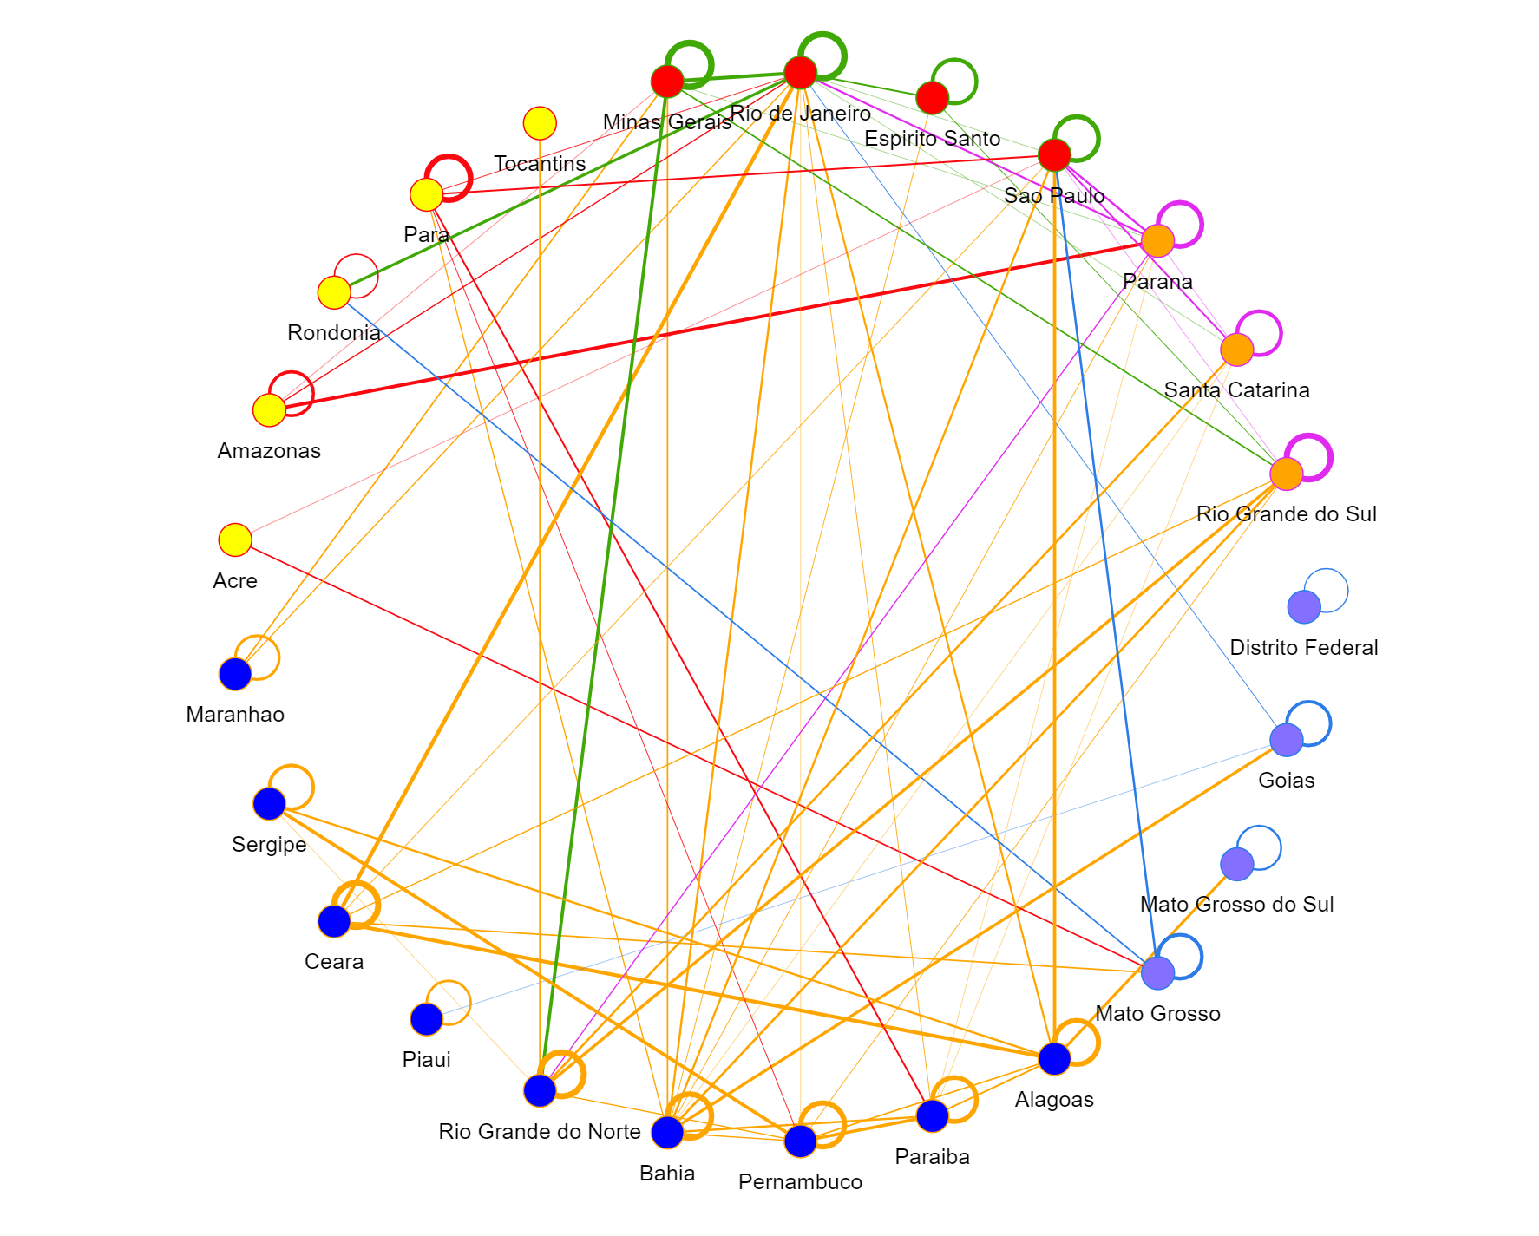
\includegraphics[width=0.35\textwidth]{Imagens/rede-exact-br-2009.pdf} &
		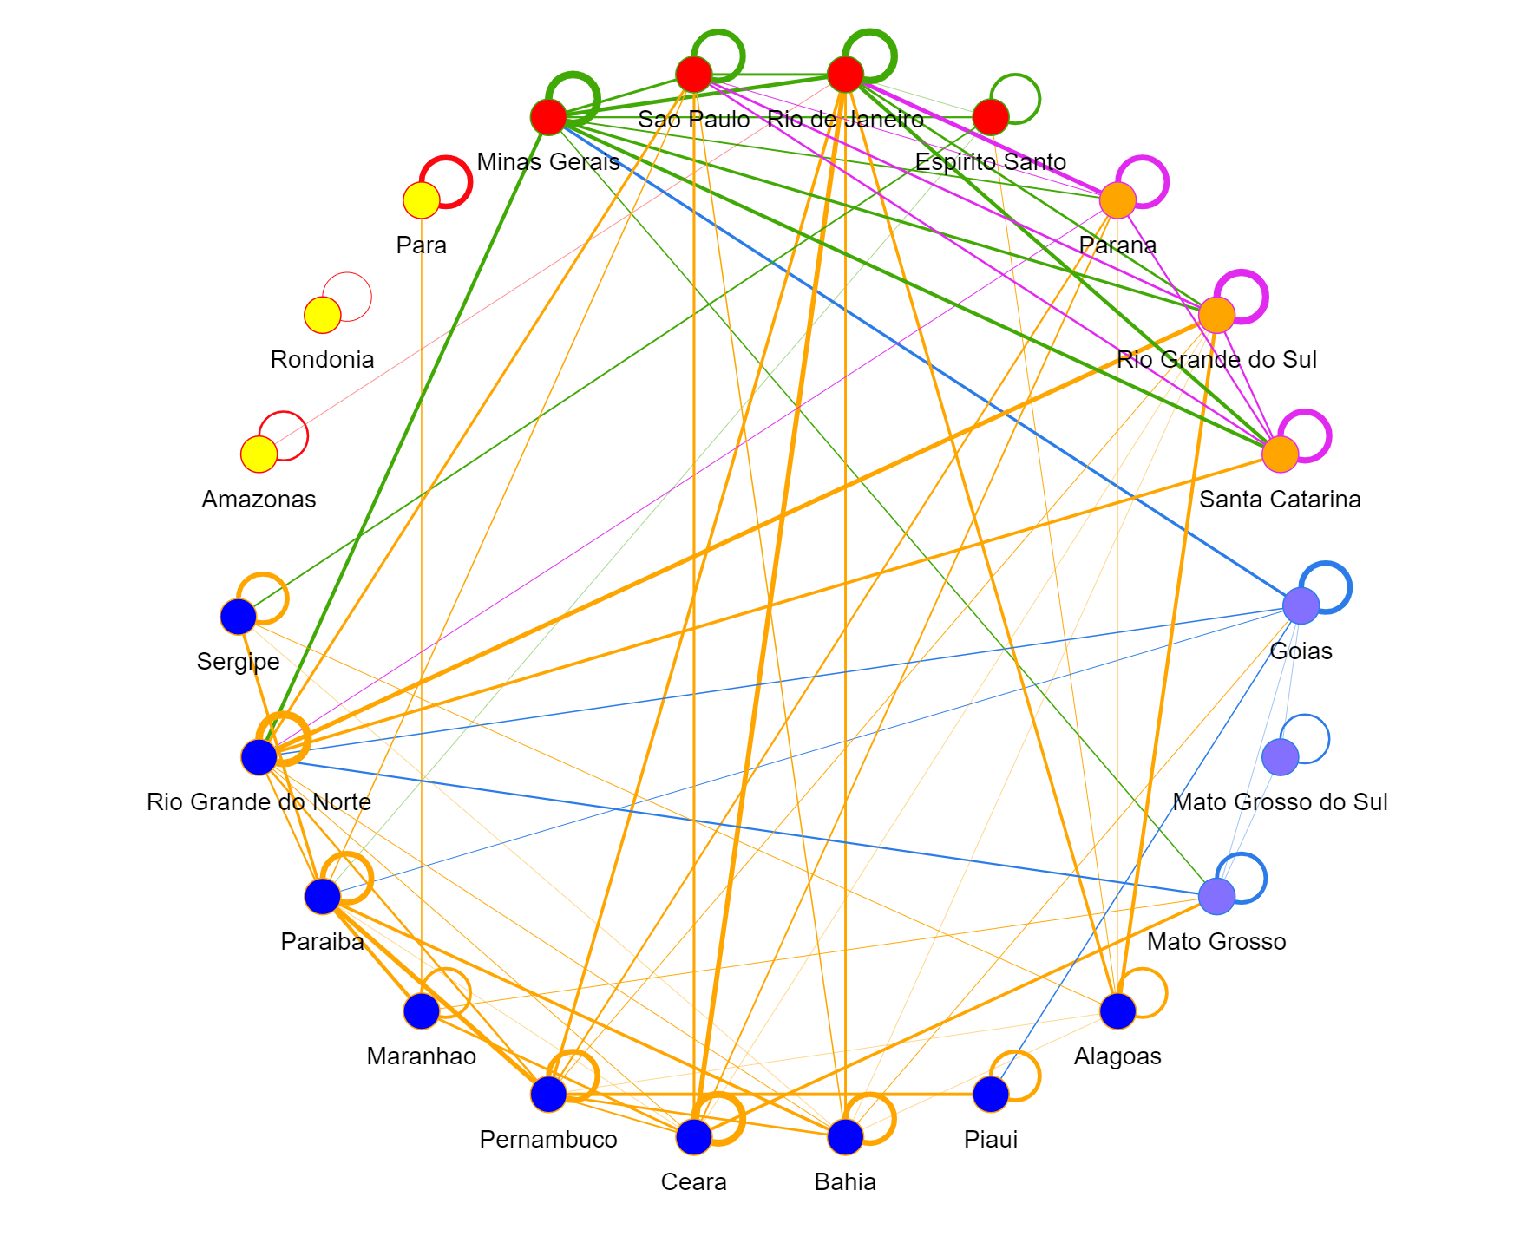
\includegraphics[width=0.35\textwidth]{Imagens/rede-exact-br-2010.pdf}\\
		2008 & 2009 & 2010\\[6pt] 
		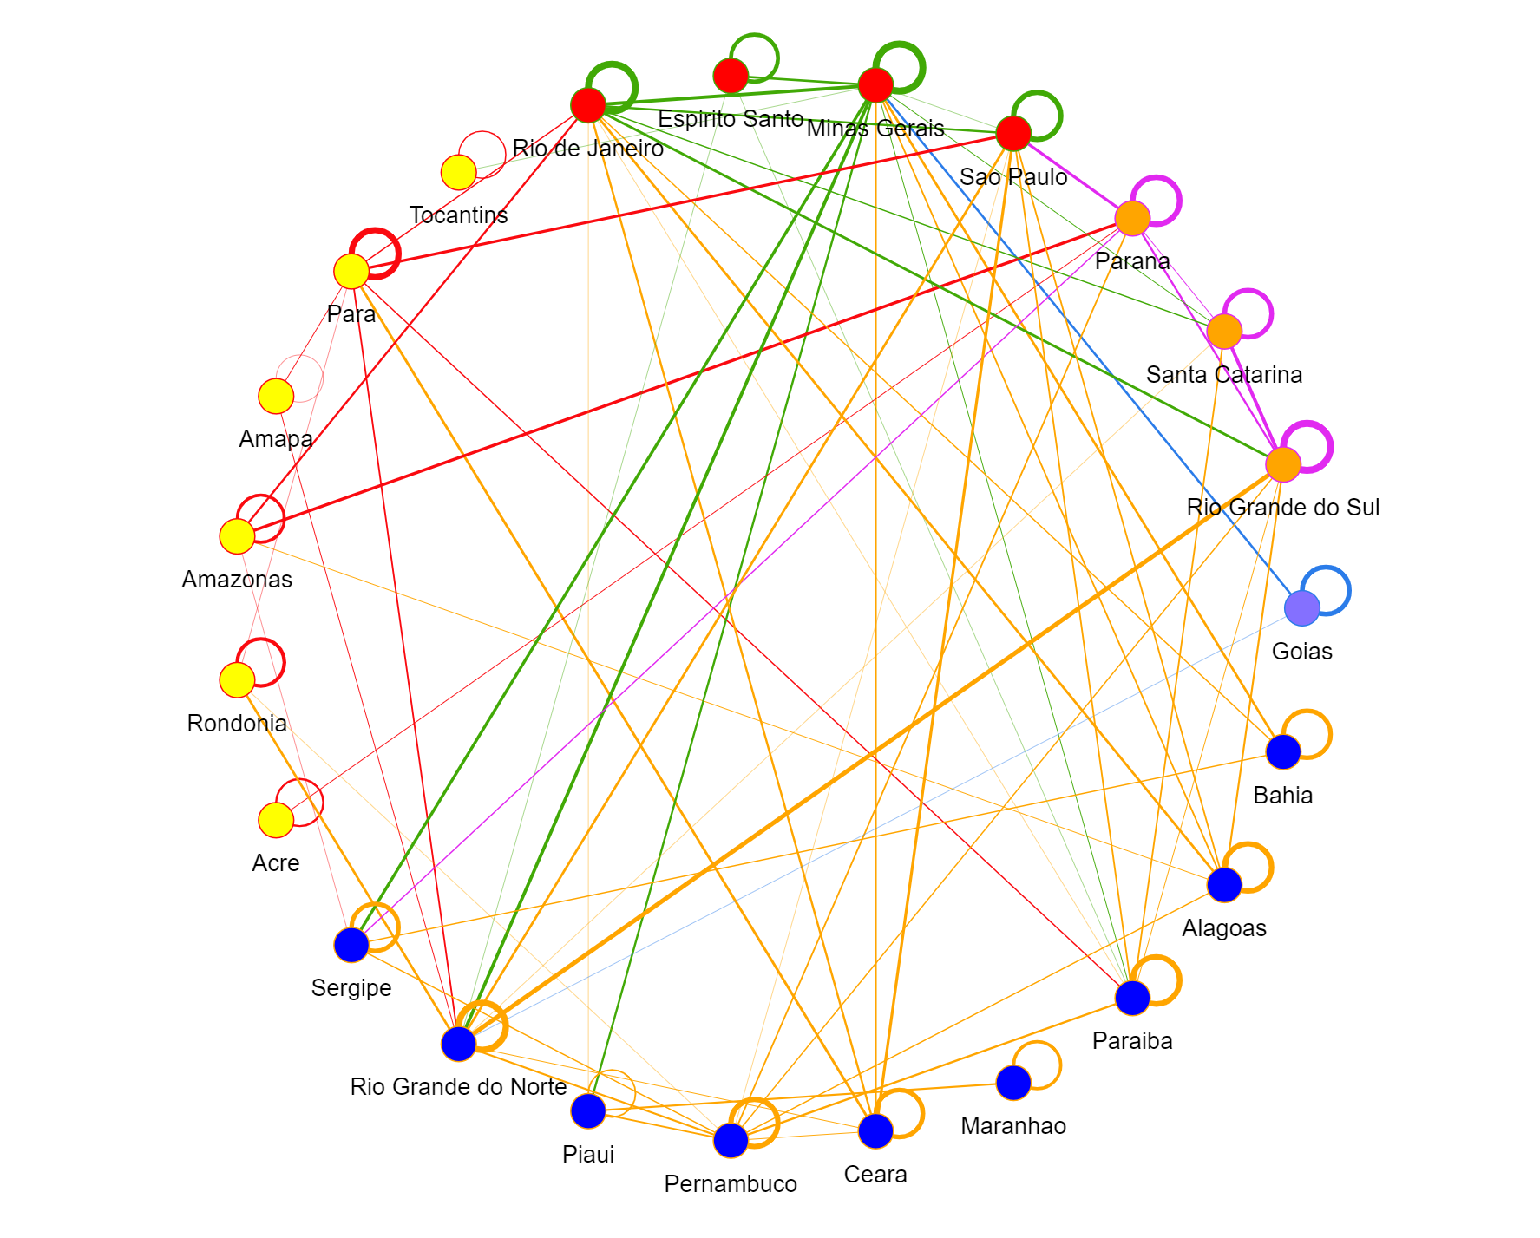
\includegraphics[width=0.35\textwidth]{Imagens/rede-exact-br-2011.pdf} &
		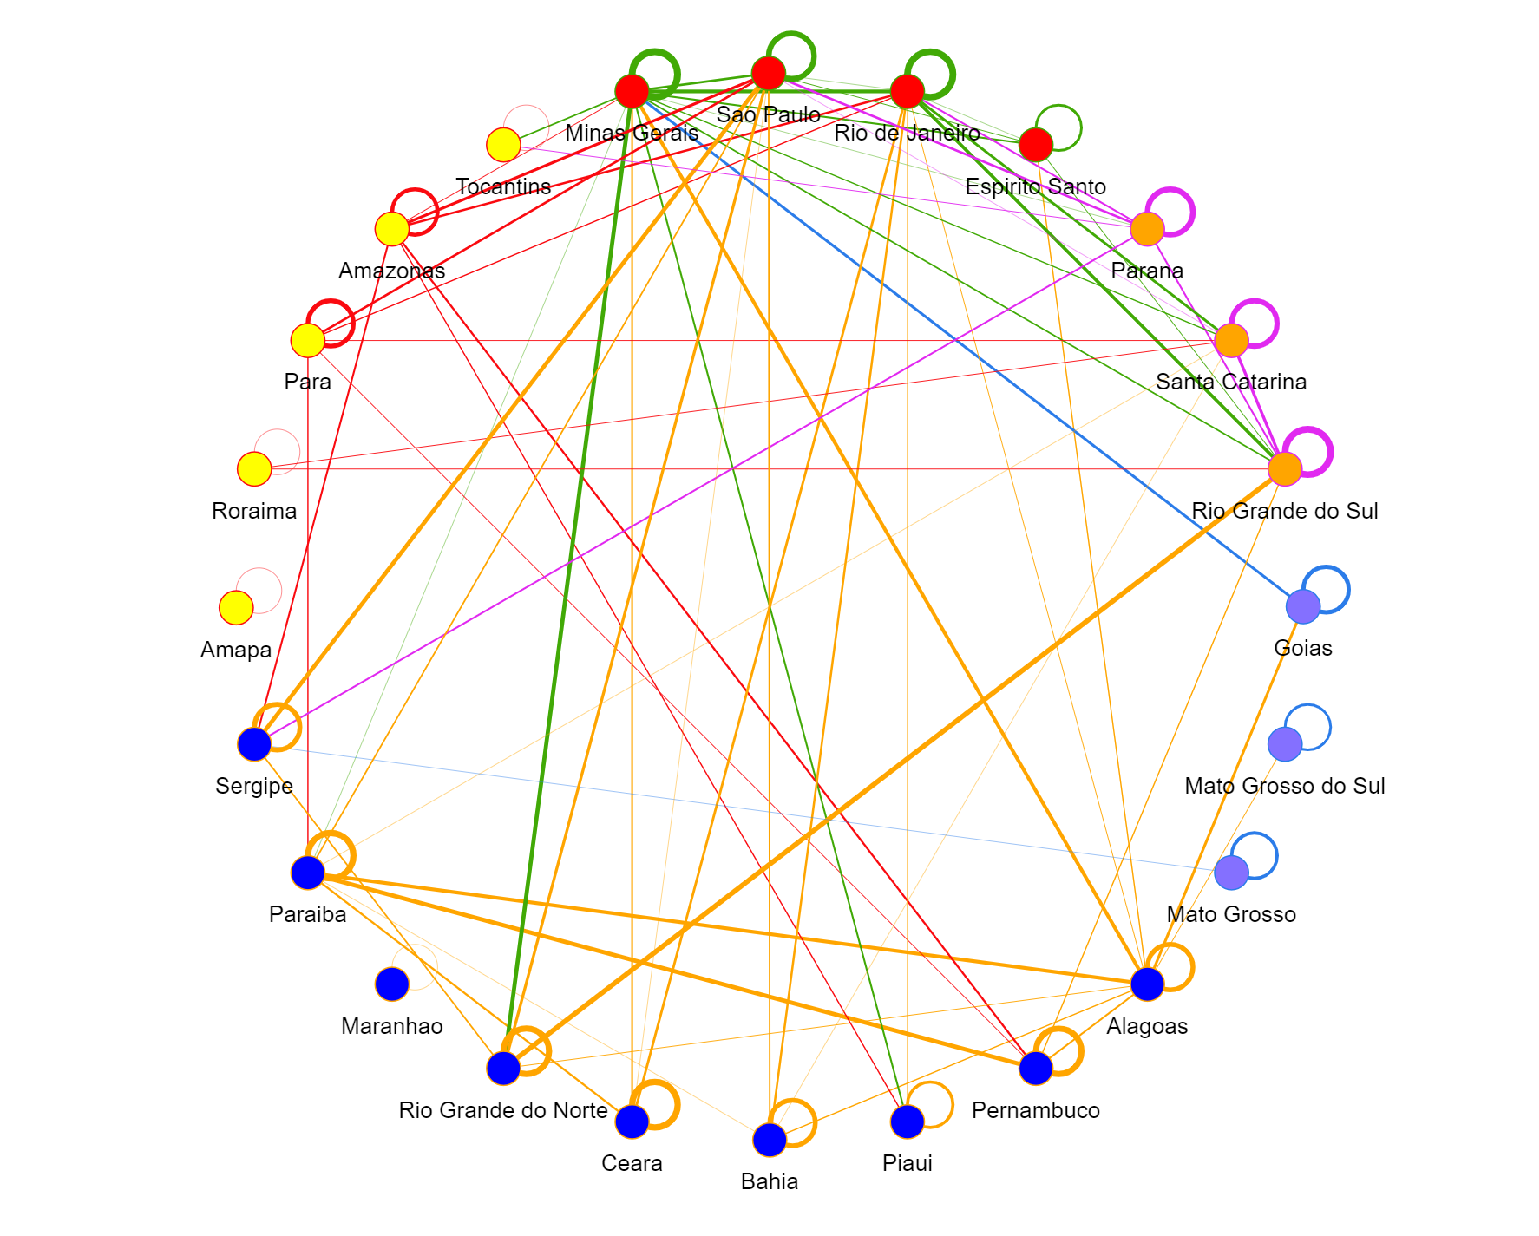
\includegraphics[width=0.35\textwidth]{Imagens/rede-exact-br-2012.pdf} &   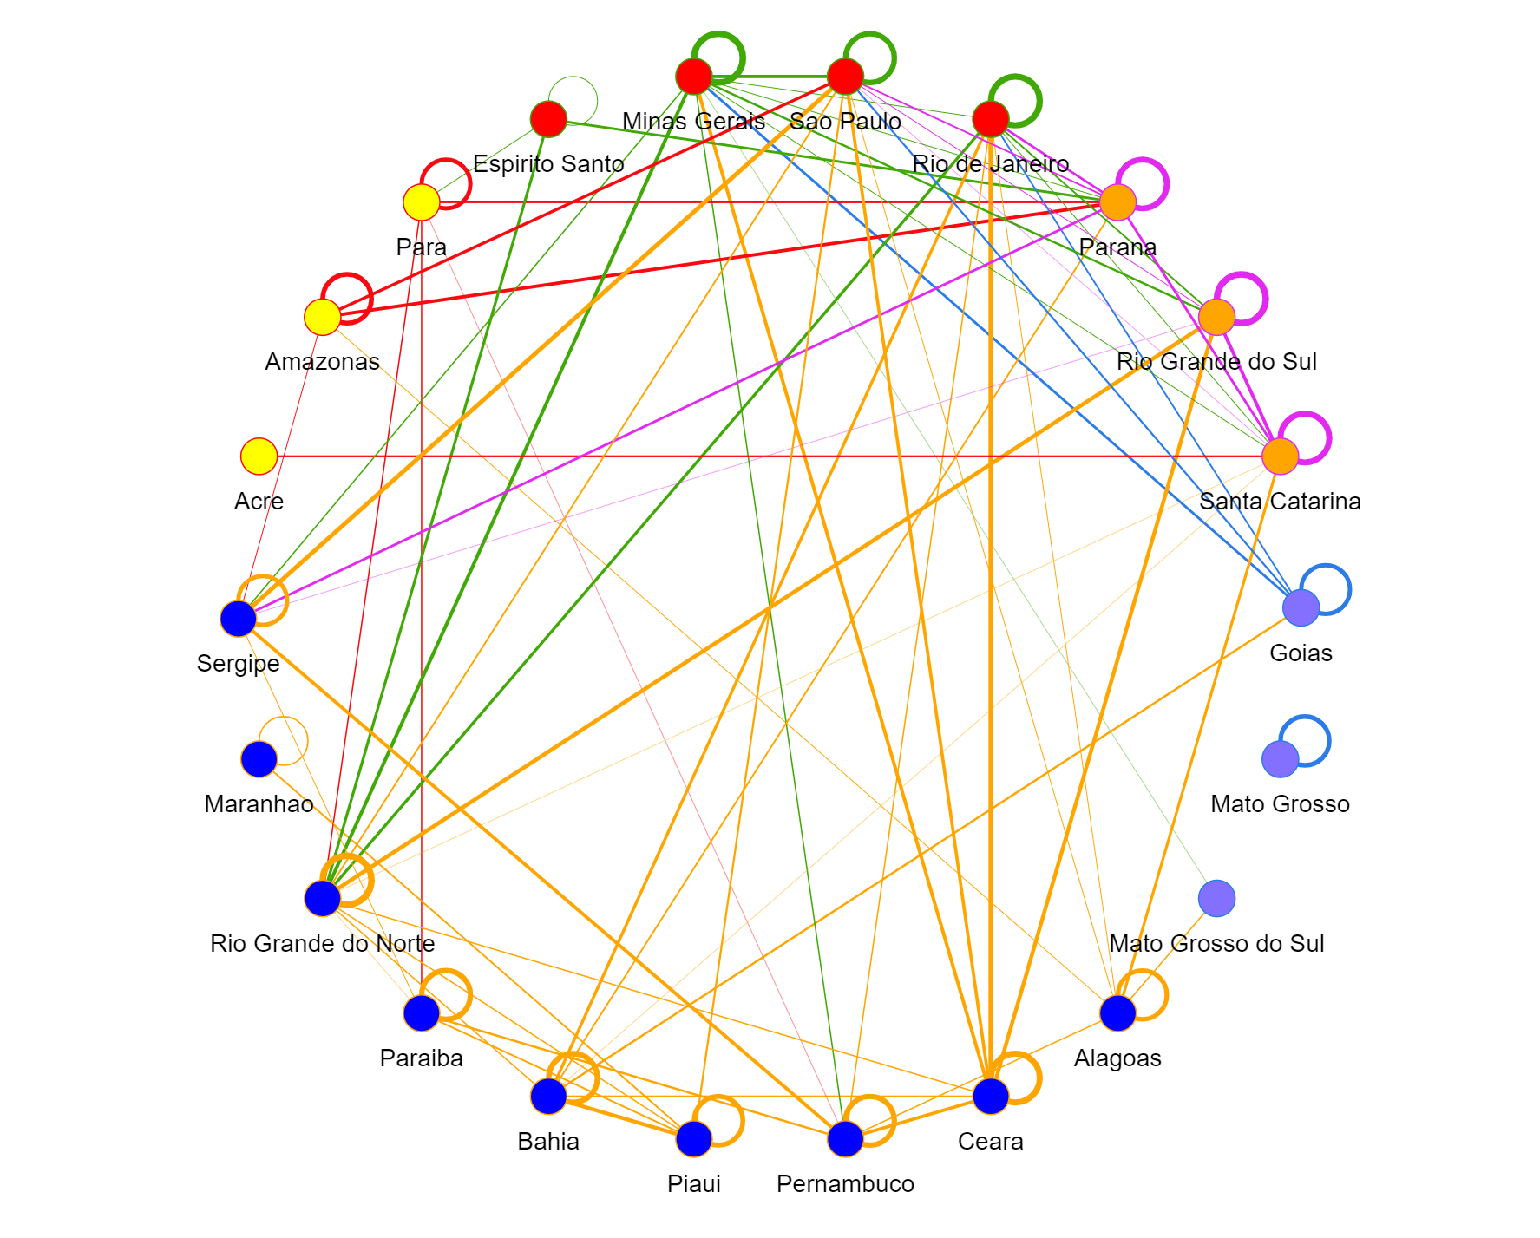
\includegraphics[width=0.35\textwidth]{Imagens/rede-exact-br-2013.pdf} \\
		2011 & 2012 & 2013\\[6pt]
		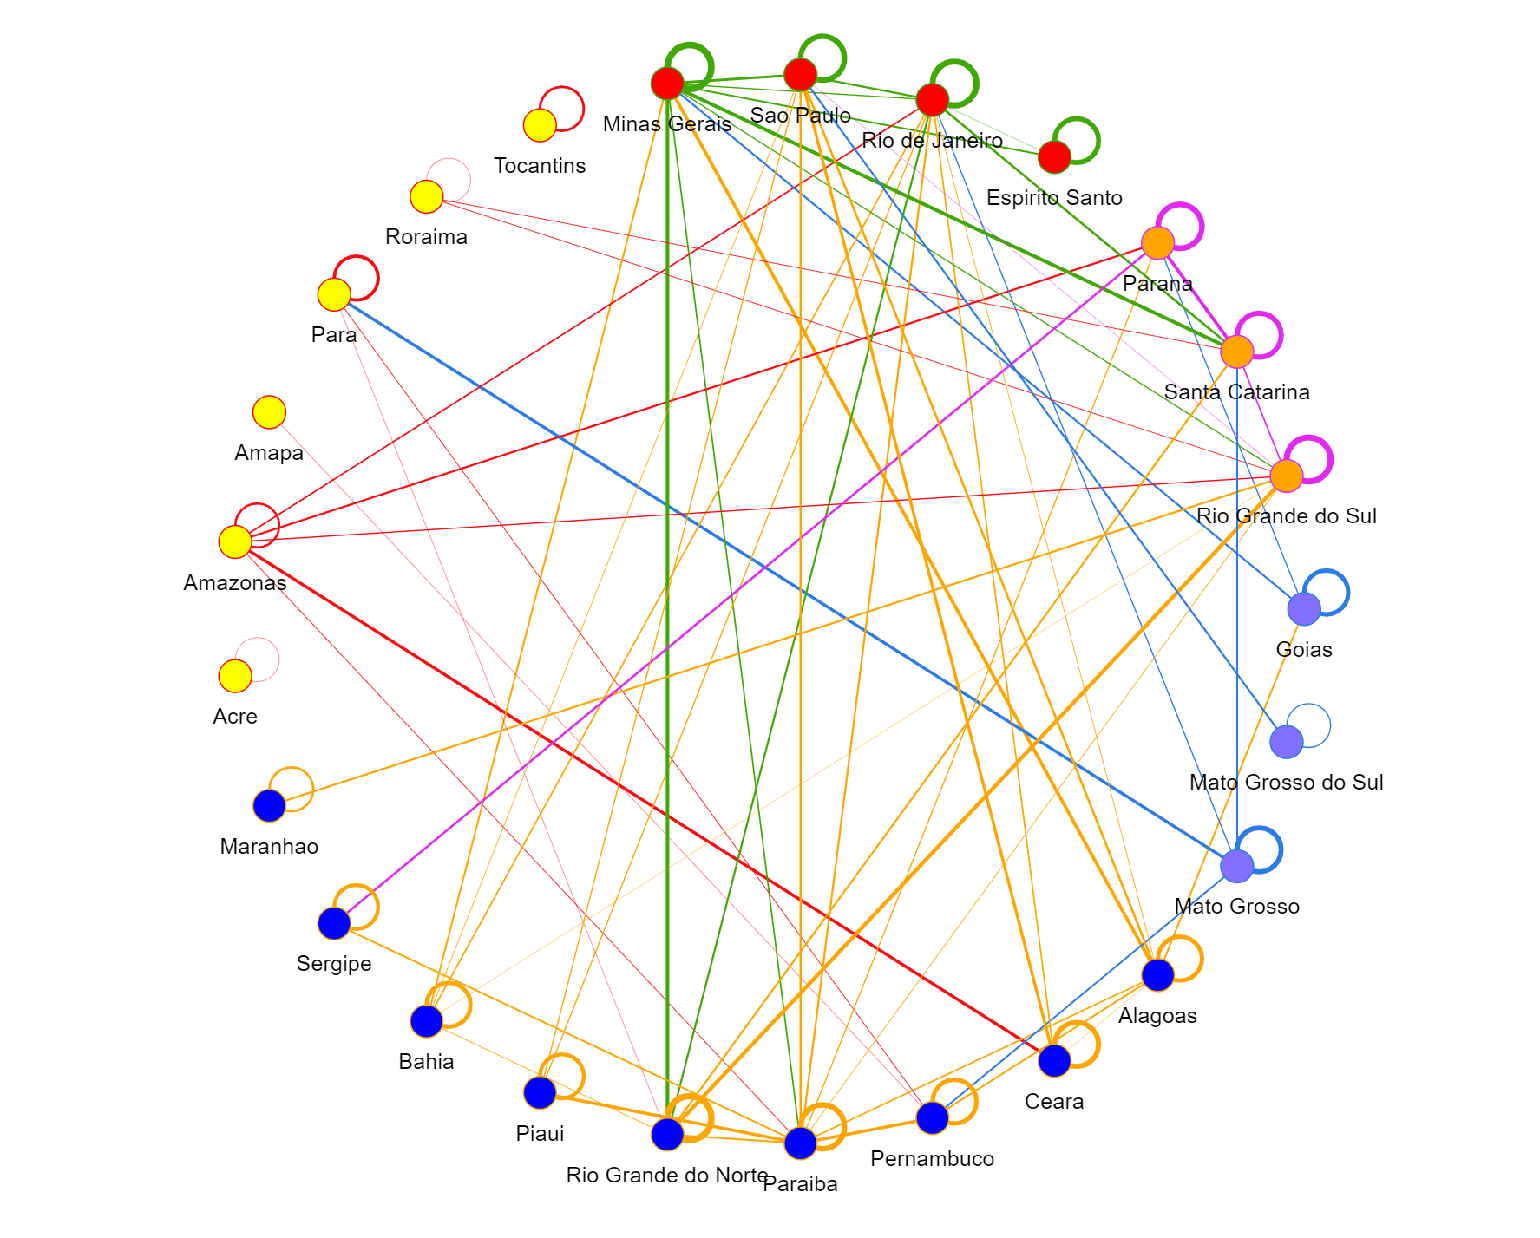
\includegraphics[width=0.35\textwidth]{Imagens/rede-exact-br-2014.pdf} &
		\includegraphics[width=0.35\textwidth]{Imagens/rede-exact-br-2015.pdf} &
		\includegraphics[width=0.35\textwidth]{Imagens/rede-exact-br-2016.pdf} \\
		2014 & 2015 & 2016\\[6pt]  \includegraphics[width=0.35\textwidth]{Imagens/rede-exact-br-2017.pdf} & & \\
		2017 & & \\
	\end{tabular}
	\caption{Redes de Coautoria Universidades Federal do Brasil - Área \textit{Exact and Earth Sciences}}
\end{figure}

\subsubsection{Rede de Coautoria Brasil - Vértice Focal Alagoas}

\begin{figure}[H]
	\begin{tabular}{ccc}
		\includegraphics[width=0.38\textwidth]{Imagens/rede-exact-AL-2008.pdf} &   \includegraphics[width=0.38\textwidth]{Imagens/rede-exact-AL-2009.pdf} &
		\includegraphics[width=0.38\textwidth]{Imagens/rede-exact-AL-2010.pdf}\\
		2008 & 2009 & 2010\\[6pt] 
		\includegraphics[width=0.38\textwidth]{Imagens/rede-exact-AL-2011.pdf} &
		\includegraphics[width=0.38\textwidth]{Imagens/rede-exact-AL-2012.pdf} &   \includegraphics[width=0.38\textwidth]{Imagens/rede-exact-AL-2013.pdf} \\
		2011 & 2012 & 2013\\[6pt]
		\includegraphics[width=0.38\textwidth]{Imagens/rede-exact-AL-2014.pdf} &
		\includegraphics[width=0.38\textwidth]{Imagens/rede-exact-AL-2015.pdf} &
		\includegraphics[width=0.38\textwidth]{Imagens/rede-exact-AL-2016.pdf} \\
		2014 & 2015 & 2016\\[6pt]  \includegraphics[width=0.38\textwidth]{Imagens/rede-exact-AL-2017.pdf} & & \\
		2017 & & \\
	\end{tabular}
	\caption{Redes de Coautoria da Universidade Federal de Alagoas  Área \textit{Exact and Earth Sciences}}
\end{figure}